\documentclass[a4paper,11pt]{article}
%\documentclass[a4paper,twoside,11pt,titlepage]{book}
\usepackage{listings}
\usepackage[utf8]{inputenc}
\usepackage[spanish]{babel}
\usepackage[backend=biber, style=alphabetic, date=year, eprint=false, isbn=false, url=false, doi=false]{biblatex} 
\usepackage{amsmath}
\usepackage{amssymb}
\usepackage{algorithm}
\usepackage{algpseudocode}
\usepackage{multirow}
\usepackage{subfig}
\usepackage{diagbox}
\usepackage{verbatim}

\addbibresource{bibliografia.bib}
\AtEveryBibitem{\clearfield{address}}
%Que no se muestren las imagenes
%\setkeys{Gin}{draft}

% \usepackage[style=list, number=none]{glossary} %
%\usepackage{titlesec}
%\usepackage{pailatino}

\decimalpoint
\usepackage{dcolumn}
\newcolumntype{.}{D{.}{\esperiod}{-1}}
\makeatletter
\addto\shorthandsspanish{\let\esperiod\es@period@code}
\makeatother


%\usepackage[chapter]{algorithm}
\RequirePackage{verbatim}
%\RequirePackage[Glenn]{fncychap}
\usepackage{fancyhdr}
\usepackage{graphicx}
\usepackage{afterpage}



\usepackage{longtable}

\usepackage[pdfborder={000}]{hyperref} %referencia
%\usepackage{cleveref}


%Math packages
\usepackage{dsfont}

% ********************************************************************
% Re-usable information
% ********************************************************************
\newcommand{\myTitle}{TFG\xspace}
\newcommand{\myDegree}{Grado en ...\xspace}
\newcommand{\myName}{Eduardo Morales Muñoz\xspace}
\newcommand{\myProf}{Pablo Mesejo Santiago\xspace}
\newcommand{\myOtherProf}{Javier Merí de la Maza\xspace}
%\newcommand{\mySupervisor}{Put name here\xspace}
\newcommand{\myFaculty}{Escuela Técnica Superior de Ingenierías Informática y de
Telecomunicación\xspace}
\newcommand{\myFacultyShort}{E.T.S. de Ingenierías Informática y de
Telecomunicación\xspace}
\newcommand{\myDepartment}{Departamento de ...\xspace}
\newcommand{\myUni}{\protect{Universidad de Granada}\xspace}
\newcommand{\myLocation}{Granada\xspace}
\newcommand{\myTime}{\today\xspace}
\newcommand{\myVersion}{Version 0.1\xspace}



\hypersetup{
pdfauthor = {\myName eedduuy@correo.ugr.es},
pdftitle = {\myTitle TFG},
pdfsubject = {},
pdfkeywords = {palabra_clave1, palabra_clave2, palabra_clave3, ...},
pdfcreator = {LaTeX con el paquete ....},
pdfproducer = {pdflatex}
}

%\hyphenation{}


%\usepackage{doxygen/doxygen}
%\usepackage{pdfpages}
\usepackage{url}
\usepackage{colortbl,longtable}
\usepackage[stable]{footmisc}
%\usepackage{index}

\makeindex
%\usepackage[style=long, cols=2,border=plain,toc=true,number=none]{glossary}
% \makeglossary

% Definición de comandos que me son tiles:
%\renewcommand{\indexname}{Índice alfabético}
%\renewcommand{\glossaryname}{Glosario}

\pagestyle{fancy}
\fancyhf{}
\fancyhead[LO]{\leftmark}
\fancyhead[RE]{\rightmark}
\fancyhead[RO,LE]{\textbf{\thepage}}
%\renewcommand{\chaptermark}[1]{\markboth{\textbf{#1}}{}}
%\renewcommand{\sectionmark}[1]{\markright{\textbf{\thesection. #1}}}

\setlength{\headheight}{1.5\headheight}

\newcommand{\HRule}{\rule{\linewidth}{0.5mm}}
%Definimos los tipos teorema, ejemplo y definición podremos usar estos tipos
%simplemente poniendo \begin{teorema} \end{teorema} ...
\newtheorem{teorema}{Teorema}[section]
\newtheorem{ejemplo}{Ejemplo}[section]
\newtheorem{definicion}{Definición}[section]
\newtheorem{proposicion}{Proposición}[section]



\definecolor{gray97}{gray}{.97}
\definecolor{gray75}{gray}{.75}
\definecolor{gray45}{gray}{.45}
\definecolor{gray30}{gray}{.94}

\lstset{ frame=Ltb,
     framerule=0.5pt,
     aboveskip=0.5cm,
     framextopmargin=3pt,
     framexbottommargin=3pt,
     framexleftmargin=0.1cm,
     framesep=0pt,
     rulesep=.4pt,
     backgroundcolor=\color{gray97},
     rulesepcolor=\color{black},
     %
     stringstyle=\ttfamily,
     showstringspaces = false,
     basicstyle=\scriptsize\ttfamily,
     commentstyle=\color{gray45},
     keywordstyle=\bfseries,
     %
     numbers=left,
     numbersep=6pt,
     numberstyle=\tiny,
     numberfirstline = false,
     breaklines=true,
   }
 
% minimizar fragmentado de listados
\lstnewenvironment{listing}[1][]
   {\lstset{#1}\pagebreak[0]}{\pagebreak[0]}

\newcommand{\bigrule}{\titlerule[0.5mm]}


%Para conseguir que en las páginas en blanco no ponga cabecerass
\makeatletter
\def\clearpage{%
  \ifvmode
    \ifnum \@dbltopnum =\m@ne
      \ifdim \pagetotal <\topskip
        \hbox{}
      \fi
    \fi
  \fi
  \newpage
  \thispagestyle{empty}
  \write\m@ne{}
  \vbox{}
  \penalty -\@Mi
}
\makeatother

\pagenumbering{roman}
\usepackage{pdfpages}
\begin{document}
\begin{titlepage}
 
 
\newlength{\centeroffset}
\setlength{\centeroffset}{-0.5\oddsidemargin}
\addtolength{\centeroffset}{0.5\evensidemargin}
\thispagestyle{empty}

\noindent\hspace*{\centeroffset}\begin{minipage}{\textwidth}

\centering

\includegraphics[width=0.7\textwidth]{Plantilla_TFG_latex/imagenes/logo_ugr.jpg}\\[1.4cm]

\textsc{ \Large TRABAJO FIN DE GRADO\\[0.2cm]}
\textsc{ Doble Grado Ingeniería Informática y Matemáticas}\\[1cm]
% Upper part of the page
% 
% Title
{\huge\bfseries Análisis del algoritmo de gradiente descendente y estudio empírico comparativo con técnicas metaheurísticas\\
}
\noindent\rule[-1ex]{\textwidth}{3pt}\\[3.5ex]

\end{minipage}

\vspace{1cm}
\noindent\hspace*{\centeroffset}\begin{minipage}{\textwidth}
\centering

\textbf{Autor}\\ {Eduardo Morales Muñoz}\\[2.5ex]
\textbf{Directores}\\
{Pablo Mesejo Santiago\\
Javier Meri de la Maza}\\[1cm]
\raggedright
\hspace{3cm}

\includegraphics[width=0.12\textwidth]{Plantilla_TFG_latex/imagenes/fcienciasLogo.png}\hspace{3.5cm}

\includegraphics[width=0.3\textwidth]{Plantilla_TFG_latex/imagenes/etsiit_logo.png} \\[0.1cm]

\centering
\vspace{0.5cm}
\textsc{Facultad de Ciencias \\ Escuela Técnica Superior de Ingenierías Informática y de Telecomunicación}\\
\textsc{---}\\
Granada, \today
\end{minipage}
%\addtolength{\textwidth}{\centeroffset}
%\vspace{\stretch{2}}
\end{titlepage}



%%\newpage
%\thispagestyle{empty}
%\mbox{}
%\newpage

\section*{Declaración de originalidad}

Yo, \textbf{Eduardo Morales Muñoz}, con DNI 77200029T, declaro explícitamente que el presente trabajo, titulado \textit{\textbf{Análisis del algoritmo de gradiente descendente y estudio empírico comparativo con técnicas metaheurísticas}}, y presentado como Trabajo de Fin de Grado (TFG), correspondiente al curso académico 2024-2025, es original, entendida esta, en el sentido de que no han sido utilizadas para la elaboración del trabajo fuentes sin citarlas debidamente.

\vspace{6cm}

\noindent Fdo: Eduardo Morales Muñoz

\vspace{2cm}

\begin{flushright}
Granada a \today.
\end{flushright}

\newpage


D. \textbf{Pablo Mesejo Santiago}, Profesor del Departamento de Ciencias de la Computación e Inteligencia Artificial de la Universidad de Granada.

\vspace{0.5cm}

D. \textbf{Francisco Javier Meri de la Maza}, Profesor del Departamento de Análisis Matemático de la Universidad de Granada.


\vspace{0.5cm}

\textbf{Informan:}

\vspace{0.5cm}

Que el presente trabajo, titulado \textit{\textbf{Análisis del algoritmo de gradiente descendente y estudio empírico comparativo con técnicas metaheurísticas}},
ha sido realizado bajo su supervisión por \textbf{Eduardo Morales Muñoz}, y autorizamos la defensa de dicho trabajo ante el tribunal que corresponda.

\vspace{0.5cm}

Y para que conste, expiden y firman el presente informe en Granada a \today.

\vspace{1cm}

\textbf{Los directores:}

\vspace{5cm}

\noindent \textbf{Pablo Mesejo Santiago \ \ \ \ \ Francisco Javier Meri de la Maza}


\newpage
%\thispagestyle{empty}
%\mbox{}
%\newpage


Yo, \textbf{Eduardo Morales Muñoz}, alumno de la titulación Doble Grado Ingeniería Informática y Matemáticas de la \textbf{Escuela Técnica Superior de Ingenierías Informática y de Telecomunicación de la Universidad de Granada}, con DNI 77200029T, autorizo la ubicación de la siguiente copia de mi Trabajo Fin de Grado en la biblioteca del centro para que pueda ser
consultada por las personas que lo deseen.

\vspace{6cm}

\noindent Fdo: Eduardo Morales Muñoz

\vspace{2cm}

\begin{flushright}
Granada a \today.
\end{flushright}



\newpage




%\newpage
%\thispagestyle{empty}
%\mbox{}
%\newpage

\section*{Agradecimientos}
\addcontentsline{toc}{section}{Agradecimientos}

       \vspace{1cm}


Gracias a mi abuelo, por hacerme ser quien soy ahora. Gracias a mis amigos y mi familia por acompañarme en este largo proceso y ofrecerme el apoyo, espacio y entendimiento. Gracias a mis tutores Javier y Pablo.


%\frontmatter
\tableofcontents
\newpage
%\listoffigures
%\listoftables
%
%\mainmatter
%\setlength{\parskip}{5pt}
\pagenumbering{arabic}
\setcounter{page}{1}
\setcounter{section}{0}
%\section{Introducción}

 %El más común es el aprendizaje supervisado \cite{mitchell1997machine}, donde la tarea $T$ es mapear una función $f$ desde unas entradas $x \in X$ hacia unas salidas $y \in Y$. Las entradas también son llamadas características y las salidas etiquetas. La experiencia $E$ es el conjunto de N parejas $\mathcal{D}=\left \{ (x_n,y_n) \right \} ^{N}_{n=1} $ que llamamos conjunto de entrenamiento. 


%En los problemas de clasificación, la salida es un conjunto no ordenado $Y= \left \{ 1,2,...,C \right \}$ donde sus elementos son denominados clases. Las tareas de clasificación de imágenes tienen un conjunto de imágenes $X$ como entrada, siendo $X=\mathds{R}^D$ donde $D=C \times D_1 \times D_2$. $C$ es el número de canales de la imágen (por ejemplo 3 si es en color RGB y 1 en escala de grises) y $D_1 \times D_2$ las dimensiones en píxeles de las imágenes.

 %Se trata también del enfoque sobre el que más se ha investigado en el aprendizae automático. \footnote{Realizando una búsqueda en Google Scholar obtenemos 6.8M de resultados para \textit{deep learning}, por encima de los 3.21M para \textit{logistic regression}, 5.51M para \textit{linear regression}, 3.58M para \textit{support vector machine} y 0.78M para \textit{gradient boosting}}. 






%Este término muchas veces se confunde con el propio algoritmo de aprendizaje (gradiente descentente), ya que aunque existen otras alternativas para este cálculo como los métodos numéricos 


%En las principales familias de modelos en cuanto a avances y resultados obtenidos como redes neuronales (ya sea convolucionales, recurrentes o con memoria), redes generativas adversarias o \textit{transformers}, el algoritmo de aprendizaje más usado es el descenso de gradiente, por ende en la mayoría está implícito el uso de \textit{backpropagation}.

%



Las metaheurísticas \cite{MHDef} son métodos de resolución que combinan procedimientos de mejora local y estrategias de alto nivel para crear un algoritmo capaz de escapar óptimos locales y desarrollar una búsqueda robusta del espacio de soluciones . Resultan especialmente útiles en problemas donde no existe una heurística específica o ésta es demasiado costosa computacionalmente, ya que pueden alcanzar soluciones cercanas a la óptima con un coste muy reducido. Su uso en el aprendizaje automático es cada vez más extendido, siendo usadas en diferentes tareas como entrenamiento de modelos, selección de hiperparámetros o elección de las arquitecturas de los modelos, con resultados diversos en cada una de estas tareas. 


%Los algoritmos genéticos \cite{MHDef} son una clase de algoritmos metaheurísticos inspirados en el proceso de selección natural y de evolución. Se basan en los principios de herencia, mutación y selección para desarrollar una población de soluciones de manera iterativa. Las soluciones son representadas como individuos o cromosomas, con una estructura dependiente del problema, y se evalúa su calidad con una función objetivo. Son una aproximación flexible y potente a la optimización, resolviendo una amplia gama de problemas de diversos ámbitos como financias, ingeniería o aprendizaje automático. Los algoritmos meméticos \cite{MHDef} son técnicas de optimización metaheurísticas basadas en la combinación de componentes de búsqueda global y local, usando conocimiento específico del problema, a diferencia de los algoritmos genéticos que no la usan. Suelen fundamentarse en estrategias basadas en población donde cada cierto número de generaciones se aplica un algoritmo de búsqueda local.


\subsection{Motivación}

Las redes neuronales profundas han permitido desarrollar modelos con muy buenos resultados en la última década y han favorecido en gran medida el desarrollo de la investigación en el aprendizaje automático. La estrategia más común que se ha tenido de entrenarlas ha sido, y sigue siendo a día de hoy, el algoritmo de gradiente descendente, por lo que están estrechamente relacionadas. La herramienta que hace posible a nivel de eficiencia computacional y escalabilidad el cálculo del gradiente y por tanto el entrenamiento de estos modelos, es \textit{backpropagation}. Aunque se estén desarrollando nuevas estrategias \cite{Metaheuristics_train} para el ajuste de pesos, sigue resultando una piedra angular y su papel en el entrenamiento de modelos desde la década de los 1990s es crucial. Estas nuevas técnicas, principalmente metaheurísticas, todavía no han logrado igualarse a las clásicas en sus resultados y costes computacionales en la tarea del ajuste de pesos, aunque se usan muy satisfactoriamente en otras tareas como la selección de hiperparámetros y arquitecturas de un modelo \cite{MHforNeuralArchAndHyper}.

Algunos problemas importantes abiertos en el campo son:

\begin{itemize}
 %   \item \textbf{Interpretabilidad}: a pesar de su gran rendimiento las redes neuronales profundas carecen totalmente de interpretabilidad, y se están desarrollando técnicas para poder explicar qué decisiones toman los modelos y por qué. \cite{interpr}

    \item \textbf{Estabilidad en el entrenamiento}: los algoritmos de aprendizaje son en general muy sensibles a la elección de los hiperparámetros y la inicialización de los pesos de los modelos, que pueden llevar a problemas de convergencia como desvanecimiento o explosión de gradiente. \cite{stabilityProblem2}

    \item \textbf{

    \item \textbf{Entender las dinámicas de optimización y las gráficas de la función de coste}: estos afectan a las propiedades de convergencia y a la propiedad de generalización. Se busca desarrollar conocimientos teóricos y herramientas prácticas para poder visualizar las trayectorias de optimización y las gráficas de la función de coste. \cite{problem4Loss&LandScape}

    \item \textbf{Sobreajuste}: ocurre cuando un modelo memoriza el conjunto de entrenamiento en lugar de aprender los patrones de los datos. Son necesarias técnicas y modelos que eviten esto y permitan generalizar el conocimiento ante datos de entrada no vistos anteriormente \cite{GoodFellowBook}.
\end{itemize}

Como vemos estos problemas se relacionan directamente con el aprendizaje, y podrían aproximarse desde dos perspectivas: buscando estrategias alternativas que mejoren al gradiente descente en la minimización del error o bien ofrecer mejoras dentro de este enfoque, ya sea con optimizadores o consiguiendo un mejor rendimiento a través de modificaciones sobre el algoritmo \textit{backpropagation}. El enfoque de este TFG es doble intentando afrontar ambas. 


En cuanto a la primera, se están desarrollando nuevas estrategias mayoritariamenta basadas en el uso de metaheurísticas como algoritmos bioinspirados. Aunque son interesantes en ciertos aspectos, aún están lejos de sustituir a las basadas en gradiente descendente debido al sobreajuste y tiempos de cálculo necesario \cite{MHtrainingClase}. Se analizarán las ventajas y desventajas de estas con respecto al enfoque clásico del gradiente descendente, realizando una descripción teórica de ambos enfoques y comparación empírica entre tres optimizadores clásicos: Adam \cite{Adam}, \textit{Nesterov Accelerated Gradient} \cite{Nesterov} y RMSProp \footnote{http://www.cs.toronto.edu/\~tijmen/csc321/slides/lecture\_slides\_lec6.pdf}; con un algoritmo genético. 


Los optimizadores son modificaciones realizadas al algoritmo de aprendizaje de descenso de gradiente para mejorar su rendimiento, ya sea acelerando la convergencia, evitando mínimos locales o mejorando la capacidad de generalización del modelo. En base a si usan sólo información del gradiente o también de la matriz hessiana, se denominan respectivamente de primer o segundo orden. En la práctica los de segundo orden no se usan ya que requieren demasiados recursos computacionales en los problemas reales, aunque tienen mejor base teórica \cite{pml1Book}. Los optimizadores de primer orden enfocan la mejora desde tres estrategias distintas: el uso del momento, \textit{learning rates} adaptativos y una combinación de los dos anteriores \cite{overview_GD}. En base a esto se ha realizado la elección de los optimizadores a usar, seleccionando uno de cada estrategia, eligiendo el más citado en el caso del momento y de la combinación (\textit{Nesterov Accelerated Gradient} y Adam) y RMSProp en el otro caso, ya que no existe artículo de publicación para contar las citaciones pero es ampliamente usado y hay resultados empíricos que demuestran un mejor rendimiento frente a otros del mismo enfoque como Adagrad \cite{AdaGrad, overview_GD}. 


Atendiendo a la segunda cuestión se investigará acerca del algoritmo \textit{backpropagation}. Se atenderá a su origen e importancia en la investigación en el aprendizaje automático y profundo, entendiendo que debido a su gran y extendido uso, una mejora aunque fuera pequeña tendría gran repercusión en campo. Para ello es necesario comprender sus bases, funcionamiento y usos, por lo que se definirá de forma detallada y se explicará su implementación práctica en librerías de programación especializadas como PyTorch \cite{PyTorch}. Además se analizarán propuestas alternativas actuales y posibles futuras. 


 %Hablar del entrenamiento, que está muy muy muy estrechamente relacionado con backprop. Parte indispensable de la mejora en el campo es la mejora en el entrenamiento, y dos partes fundamentales de esto son mejorar backprop y mejorar la manera de ajustar los pesos. En cuanto a la primera se trata de lo más usado a nivel general, y en cada proceso de entrenamiento se usa tantas veces que cualquier cambio supondrá una mejora sustancial, por ello para poder proporcionar alguna mejora hay que entender qué es, en qué se basa y cómo se usa.

%En cuanto a lo segundo, hay muchas maneras de entrenamiento de redes neuronales, la mas comun es descenso de gradiente, pero hay más. Tanto dentro como fuera del ambito de descenso de gradiente la literatura puede ser liosa. Queda claro que actualmente gradiente descendente es mejor pero ahí dentro hay muchas opciones y literatura confusa. Fuera hay opciones interesantes pero que no están asentadas. Describirlas y realizar una comparación, proponiendo una nueva.

\subsection{Objetivos}

El objetivo principal de este TFG es investigar acerca de la posibilidad de mejoras en las técnicas de entrenamiento de modelos en aprendizaje profundo, revisando para ello las técnicas clásicas basadas en gradiente descendiente y alternativas metaheurísticas. Se definen por tanto los siguiente objetivos y objetivos parciales:



    \item Realizar una investigación teórica entre los enfoques de entrenamiento clásico basados en descenso de gradiente y las técnicas metaheurísticas, justificando la superioridad actual de las técnicas clásicas. 

    \begin{enumerate}
        \item Investigación sobre los optimizadores de primer orden del descenso de gradiente, analizando su base teórica, ventajas y desventajas.

        \item Investigación de las técnicas metaheurísticas para el ajuste de pesos en los modelos, analizando sus ventajas y desventajas con respecto a las técnicas clásicas.

        
    \end{enumerate}

    \item Realizar pruebas experimentales usando optimizadores de primer orden. Realizar una propuesta de técnica metaheurística y realizar desarrollo teórico y empírico. Dividimos entre los siguientes sobjetivos parciales:

    \begin{enumerate}
        \item Realización de pruebas experimentales de los tres optimizadores elegidos, comparando los resultados entre sí para analizar las ventajas y desventajas de cada estrategia.

        \item Describir una propuesta de algoritmo genético y memético y realizar un desarrollo tanto teórico como empírico, comparándolo con los resultados obtenidos en el objetivo anterior.
    \end{enumerate}
\end{enumerate}





\newpage

%\part{Parte matemática: gradiente descendente y \textit{backpropagation}}
\vspace{4cm}

\newpage 

\part{Parte matemática: análisis del gradiente descendente, su convergencia y \textit{backpropagation}.}

\newpage


\section{Introducción}

El aprendizaje automático es una rama de la inteligencia artifical en la que los sistemas son capaces de adquirir conocimiento a partir de datos sin procesar \cite{GoodFellowBook}. Se dice que un programa aprende de la experiencia $E$ respecto de alguna tarea $T$ y una medición de rendimiento $P$ si su rendimiento en $T$, medido por $P$, mejora con la experiencia $E$ \cite{mitchell1997machine}. Nos referimos a este programa como modelo. Existen muchos tipos o subramas de aprendizaje automático dependiendo de la naturaleza de esta tarea $T$ y de su medidor de rendimiento $P$. 

El entrenamiento de un modelo es el proceso de optimizar sus parámetros (equivalentemente pesos), es decir, su representación interna; para minimizar una función de coste (equivalentemente función de error o de pérdida) $C$ que mide el error en el rendimiento. El dominio de dicha función es el espacio de valores que pueden tomar los pesos, normalmente representado de forma tensorial; y su imagen es comúnmente un real no negativo. El objetivo principal del entrenamiento es que el modelo sea capaz de aprender los patrones en un conjunto de datos para luego poder generalizarlos en otros que no ha visto previamente. Diremos que existe un sobreajuste cuando se aprenden los patrones específicos de los datos pero luego no se generaliza bien. La estrategia que usamos para optimizar los pesos es llamada algoritmo de aprendizaje.

El aprendizaje profundo es un paradigma del aprendizaje automático en el que los modelos tienen varios niveles de representación obtenidos a través de la composición de módulos sencillos pero comúnmente no lineales, que transforman la representación de los datos sin procesar hacia un nivel de abstracción mayor \cite{lecun2015deep}. Esta rama comenzó a ganar peso en la década de los 2000 y un punto de inflexión fue el resultado de la competición de ImageNet \footnote{http://www.image-net.org/challenges/LSVRC/} en 2012 \cite{NIPS2012_c399862d}. Actualmente este enfoque es el que mejores resultados consigue, siendo una parte fundamental en la investigación y estructura de las grandes compañías tecnológicas y pudiendo ofrecer aplicaciones comerciales a nivel usuario \cite{Sejnowski18, lecunnDeepForAI}.

La mayoría de los modelos en aprendizaje automático se entrenan usando técnicas basadas en el algoritmo de aprendizaje de gradiente descendente (equivalentemente descenso del gradiente), ya que es la estrategia que mejores resultados ofrece actualmente en cuanto a capacidad de generalización del modelo y rendimiento computacional \cite{GoodFellowBook, CauchyGD}. Ésta se basa en la idea de que puedo moverme hacia puntos de menor valor en la función de error del modelo realizando pequeños movimientos en  sentido contrario a su gradiente como se esquematiza en la figura \ref{fig:1.GD}, con el objetivo de minimizar el valor de salida. Al tratarse de un algoritmo iterativo, es fundamental estudiar su convergencia, que depende de varios factores y se enfrenta a diversas dificultades, como veremos en secciones posteriores.

El algoritmo de \textit{backpropagation} (BP) permite transmitir la información desde la salida de la función de coste hacia atrás en un modelo con varios módulos de abstracción para así poder computar el gradiente de una manera sencilla y eficiente \cite{rumelbackprop}. Aunque existen otras posibilidades a la hora de realizar éste cómputo, BP es la más usada y extendida gracias a propiedades como su flexibilidad, eficiencia y escalabilidad, que lo hacen destacar por encima de otras opciones \cite{GoodFellowBook}. 

\begin{figure}
    \centering
    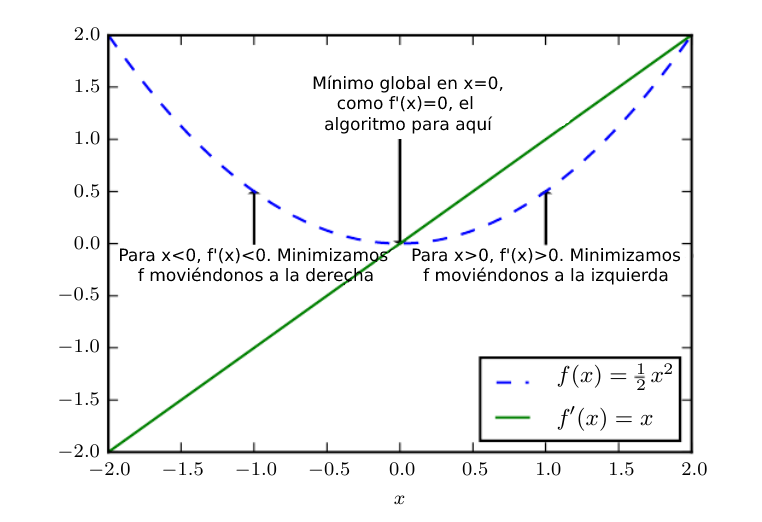
\includegraphics[width=0.75\linewidth]{Plantilla_TFG_latex//imagenes//Mat//1.intro/1.1GDMatIntroGoodFellowBook.png}
    \caption{Esquematización de la estrategia de descenso del gradiente en un modelo con un solo parámetro x. El eje horizontal representa los valores que toma éste y el vertical representa el error del modelo en función de x. Imagen obtenida y traducida del libro \cite{GoodFellowBook}}
    \label{fig:1.GD}
\end{figure}



Dependiendo de la familia de modelos que usemos podremos utilizar una estrategia de aprendizaje distinta, como el caso del \textit{Perceptron} y su \textit{Perceptron Learning Algorithm} \cite{patternrecog}. En otros casos como la regresión lineal se usa la estrategia de descenso de gradiente pero el gradiente no tiene por qué calcularse a través de BP. Esto se debe a que en este caso se puede obtener eficientemente a través de librerías matemáticas como \textit{numpy} \footnote{https://numpy.org/} en el caso del lenguaje \textit{python} \footnote{https://es.python.org/}, ya que esta familia de modelos conllevan menos costo computacional en sus cálculos principalmente debido al escaso número de parámetros en comparación con los de aprendizaje profundo. Para éste sí que es necesario el uso de BP en el caso de que elijamos entrenar mediante gradiente descendente, ya que aunque existen otras alternativas como los métodos numéricos o algunas aproximaciones recientes , no consiguen igualar su rendimiento \cite{EffBackProp, GoodFellowBook, alternativabacknumerical, alternativabackprop1}.


Otra de las características de este algoritmo para el cálculo del gradiente es que los conceptos en los que se basa son simples: optimización, diferenciación, derivadas parciales y regla de la cadena. Lo cual lo convierte a priori en objeto de estudio accesible. En la práctica, los cálculos que se realizan en esta estrategia se implementan a través de la diferenciación automática, que es una técnica más general que extiende a BP y se usa para el cómputo de derivadas de funciones numéricas de una manera eficiente y precisa \cite{AutomaticDiff}.% Ésta aprovecha el hecho de que cada cálculo que se realiza en un ordenador queda reducido a una secuencia de operaciones aritméticas elementales (suma, resta, multiplicación...) y funciones elementales (exponencial, trigonométricas, ...) para aplicar de forma repetida la regla de la cadena a estos elementos básicos hasta poder obtener derivadas de orden arbitrario. 



\subsection{Motivación}

Tenemos pues que el aprendizaje profundo es el paradigma del aprendizaje automático que mejores resultados obtiene actualmente y más desarrollo e investigación está concentrando, y que basa el entrenamiento (una de las partes fundamentales que determinan el rendimiento del modelo, además de su arquitectura) de los modelos casi por completo en el algoritmo de descenso de gradiente, ya que es el que mejores resultados de generalización ofrece. Éste a su vez depende casi enteramente del algoritmo de BP para calcular el gradiente, ya que aunque existan otras alternativas no son realmente viables. Tanto es así que es muy común la confusión entre éste algoritmo y el de gradiente descentente, que se suelen tomar por la misma cosa. Queda así clara la importancia que tiene BP en el campo del aprendizaje profundo y por extensión también al aprendizaje automático. También conviene destacar la cantidad de veces que se utiliza ésta técnica durante el entrenamiento de un modelo. Cada vez que se actualizan los pesos debemos calcular el gradiente, y teniendo en cuenta la duración de los entrenamientos de los modelos más grandes (con mayor número de parámetros) este algoritmo puede ser usado miles de veces durante un entrenamiento.

Su eficiencia, escalabilidad y flexibilidad lo han convertido en la opción por defecto para el entrenamiento basado en gradiente descendente para modelos de aprendizaje profundo, sin embargo no hay que olvidar que no se trata de una tarea sencilla: la obtención de un mínimo global y la verificación, dado un punto, de que es un mínimo global, se trata de un problema NP-Completo generalmente \cite{NPHardProblem}, por lo que se buscan estrategias aproximadas capaces de obtener buenas soluciones en tiempos razonables. Uno de los problemas abiertos en el aprendizaje profundo y en el que influye directamente BP es la reducción computacional del entrenamiento: si se ajustan los pesos en un modelo con un número muy alto de parámetros y usando un conjunto de entrenamiento muy grande (que es una tendencia reciente en aprendizaje profundo), los recursos computacionales pueden resultar insuficientes incluso para las grandes compañías, pudiendo requerir de meses para el  entrenamiento. Por lo que se necesitan algoritmos más escalables y eficientes para afrontarlo \cite{Problem3_accel}.

Por ello resulta esencial, mientras no existan alternativas viables, poder ofrecer modificaciones a este algoritmo para mejorar sus cualidades. Atendiendo a la cantidad de uso y su extensión en el campo, una pequeña mejora tendría un alcance enorme. Sin embargo esta línea de investigación no es muy extensa ya que principalmente se buscan alternativas en lugar de mejoras, pudiendo deberse principalmente a que a priori puede parecer una técnica muy enrevesada y compleja. Veremos en el desarrollo de esta parte que esto no es cierto, y que los principios en los que se basa son muy simples. Es clave comprender su base teórica, funcionamiento e implementación práctica para poder proponer mejoras. 


\subsection{Objetivos}

El objetivo principal de esta parte es realizar una investigación sobre los algoritmos de descenso de gradiente y \textit{backpropagation}, proporcionando una visión detallada acerca de los mismos y su implementación. Para ello se divide este objetivo en varios:

\begin{enumerate}
    %\item Exposición de la importancia actual e histórica en el campo del aprendizaje automático y aprendizaje profundo, viendo su estrecha relación con el algoritmo de aprendizaje del gradiente descente.

    
    \item Definir de manera detallada la base teórica y funcionamiento del algoritmo de descenso de gradiente atendiendo a elementos clave como su convergencia. Enunciar y demostrar resultados teóricos sobre la convergencia y analizar los problemas de ésta.

    \item Explorar el uso de BP para el cálculo del gradiente, analizando su implementación a través de la diferenciación automática.

    %\item Analizar de modo teórico las principales variantes del algoritmo de descenso de gradiente. 

 %   \item Realizar una investigación y revisión teórica de las alternativas al cálculo de gradiente basadas en otras estrategias como los métodos numéricos, e inviabilidad de las mismas frente a BP.
\end{enumerate}







\section{Fundamentos previos}
A continuación se definirán los conceptos básicos necesarios con los que se trabajará durante el desarrollo de esta parte. Se tratarán los elementos necesarios que se usan en el algoritmo de gradiente descendente y BP. Se presenta únicamente el material estrictamente necesario para comprender el trabajo. Se ha usado para la elaboración de esta sección los apuntes en línea del profesor de la UGR Rafael Payá Albert en su curso de Análisis Matemático I \footnote{\url{https://www.ugr.es/~rpaya/docencia.htm\#Analisis}}.  Salvo otras especificaciones, el material de consulta para el desarrollo de esta parte matemática ha sido el curso en línea de Ciencias de Computación de la universidad Bristish Columbia \footnote{\url{https://www.cs.ubc.ca/~schmidtm/Courses/5XX-S22/}} y los libros Probabilistic Machine Learning \cite{murphy2022probabilistic} y Deep Learning \cite{GoodFellowBook}


\subsection{Cálculo diferencial}

A continuación se definirán los principales conceptos que se usarán durante el presente TFG. Los algoritmos de gradiente descendente y BP se basan principalmente en el cálculo diferencial, y el hecho de que no usen herramientas matemáticas demasiado complejas resulta precisamente una de sus virtudes, ya que gracias a la abstracción y a un diseño ingenioso consiguen obtener grandes resultados a partir de operaciones relativamente sencillas. Empezamos con los conceptos más elementales que subyacen durante todo el trabajo.

Tomaremos $X$ e $Y$ como dos espacios normados no triviales cualesquiera. Se fija una función $f:A \rightarrow Y$ donde $\varnothing \neq A\subseteq X$ y un punto $a \in A^{\circ}$

\begin{definicion}[Función diferenciable]
    $f$ es diferenciable en el punto $a$ si existe una aplicación lineal y continua $T \in L(X,Y)$ que verifica:

    $$\displaystyle \lim_{x \to a} \frac{\left\| f(x)-f(a)-T(x-a)\right\|}{\left\| x-a\right\|}=0$$
    
    Decimos que $f$ es diferenciable si es diferenciable en todo punto del interior de su dominio.
\end{definicion}


\begin{definicion}[Derivada parcial]
        Sea $f: \Omega \subset \mathbb{R}^n \rightarrow Y \subset \mathbb{R}^M$, con $\Omega$ un abierto, $f=(f_1, f_2, ..., f_M)$, $a \in \Omega$, $k \in I_n$. Entonces $f$ es parcialmente derivable con respecto a la $k$-ésima variable en $a$ si, y sólo si, lo es $f_j \forall j \in I_M$, en tal caso, 

        $$\frac{\partial f}{\partial x_k}(a) = \left ( \frac{\partial f_1}{\partial x_k}(a), ..., \frac{\partial f_M}{\partial x_k}(a) \right ) \in \mathbb{R}^M$$

        $f$ es parcialmente derivable en $a$ si, y sólo si, lo es respecto de todas sus variables
\end{definicion}


Definimos ahora los elementos clave del proceso: el vector gradiente y la matriz jacobiana. En el algoritmo de descenso de gradiente, lo que se pretende calcular tal como indica el nombre es el vector gradiente, ya que la función de error de los modelos siempre nos devuelve un escalar, es decir que la dimensión de la imagen es 1, y la dimensión de la entrada será el número de parámetros del modelo (número de elementos que tendrá el vector gradiente). Sin embargo las matrices jacobianas también juegan un papel fundamental ya que para calcular ese vector gradiente, el algoritmo de BP necesita de cálculos intermedios, que son las matrices jacobianas asociadas entradas y salidas de las capas ocultas (que tienen mayor dimensionalidad) con respecto a parte de los parámetros (los parámetros de esa capa). 

\begin{definicion}[Vector gradiente]
    Sea $f:\Omega \subset \mathbb{R}^N \rightarrow \mathbb{R}$ un campo escalar, con $\Omega$ un abierto y $a \in \Omega$ . Cuando $f$ es parcialmente derivable en $a$, el gradiente de $f$ en $a$ es el vector $\nabla f(a) \in \mathbb{R}^N$ dado por 
    $$\nabla f(a) = \left ( \frac{\partial f}{\partial x_1} (a), \frac{\partial f}{\partial x_2} (a), ..., \frac{\partial f}{\partial x_N} (a) \right )$$
\end{definicion}


Fijamos un abierto $\Omega \subset \mathbb{R}^N$
, y la función $f:\Omega \rightarrow \mathbb{R}^M$. Notamos por $f= \left ( f_1,f_2,..., f_M \right )$ indicando las $M$ componentes de $f$ que son campos escalares definidos en $\Omega$, siendo $f_j=\pi _j \circ f$.

\begin{definicion}[Matriz jacobiana]
    Si $f$ es diferenciable en $ x \in \Omega$, la matriz jacobiana es la matriz de la aplicación lineal $Df \in L \left ( \mathbb{R}^N, \mathbb{R}^M \right )$ y se escribe como $J_f$. Viene dada por:

    $$J_f(x)= \begin{pmatrix}
 \frac{\partial f_1}{\partial x_1} & \frac{\partial f_1}{\partial x_2} & \cdots & \frac{\partial f_1}{\partial x_N} \\
 \frac{\partial f_2}{\partial x_1} & \frac{\partial f_2}{\partial x_2} & \cdots & \frac{\partial f_2}{\partial x_N} \\
 \vdots & \vdots & \ddots & \vdots \\
 \frac{\partial f_M}{\partial x_1} & \frac{\partial f_M}{\partial x_2} & \cdots & \frac{\partial f_M}{\partial x_N} \\
\end{pmatrix}= \begin{pmatrix}
 \nabla f_1(x)^T\\
 \vdots \\
 \nabla f_M(x)^T \\
\end{pmatrix}=
\begin{pmatrix}
     \frac{\partial f}{\partial x_1} \cdots \frac{\partial f}{\partial x_N}
\end{pmatrix}$$
\end{definicion}


Se presenta a continuación una de las reglas más útiles para el cálculo de diferenciales, que afirma que la composición de aplicaciones preserva la diferenciabilidad. Será parte clave en el desarrollo próximo ya que a los modelos de aprendizaje automático basados en capas podemos describirlos como una función que se descompone en una función por cada capa, por tanto será una herramienta que usaremos continuamente para calcular estas matrices jacobianas y gradientes.

\begin{teorema}[Regla de la cadena]
    Sean $X, Y, Z $ espacios normados, $\Omega$ un abierto no vacío de $X$ y $U$ lo es de $Y$, y las funciones $f:\Omega \rightarrow U$ y $g:U \rightarrow Z$. Entonces si $f$ es diferenciable en $a \in \Omega$ y g es diferenciable en $b=f(a)$ se tiene que $f \circ f$ es diferenciable en $a$ con

    $$D(g \circ f)(a) = Dg(b) \circ Df(a) = Dg(f(a)) \circ f(a)$$

    \raggedright{Si $f \in D(\Omega, Y)$ y  $g \in D(U,Z)$, entonces $g \circ f \in D(\Omega, Z)$.}
    
\end{teorema}


En ocasiones en algunos modelos tenemos que lidiar con funciones que no son diferenciables en un punto, y para poder manejarlas extenderemos el concepto de diferenciabilidad a lo que llamaremos subdiferenciabilidad. Esto se expondrá más adelante ya que son conceptos que no se han explorado a lo largo del grado de matemáticas.



\begin{comment} %Esto creo que no lo uso
	\begin{definicion}[Función continuamente diferenciable]
	    Si una función $f$ parcialmente derivable tiene todas sus derivadas parciales continuas, decimos que la función $f$ es continuamente diferenciable. Decimos que es de clase $C^1$.
	\end{definicion}
\end{comment}


\begin{comment}
    
	
	\begin{definicion}[Conjunto conexo]
	    Un espacio métrico $E$ es convexo si no puede ser expresado como unión de dos subconjuntos abiertos, no vacíos y disjuntos. Podemos formularlo de la siguiente manera:
	
	    $$U=U^{\circ}, V=V^{\circ}, U \cup V = E, U \cap V = \emptyset \Rightarrow U=\emptyset ó V=\emptyset$$
	\end{definicion}
	
	Caracterizamos de manera sencilla un espacio conexo:
	
	\begin{itemize}
	    \item \textit{Un espacio métrico $E$ es conexo si, y sólo si, para cualesquiera dos puntos $x,y \in E$ existe un conjunto conexo $C \subset E$, tal que $x,y \in C$}
	\end{itemize}
	
	Podemos decir de esta manera que un espacio métrico $E$ es conexo cuando cualquiera dos puntos de $E$ están conectados, es decir, existe un subconjunto conexo de E que los contiene.

\end{comment}




\begin{comment}
	
	\begin{definicion}[Función estrictamente convexa]
	    Sea $E \subset \mathbb{R}^n$ un conjunto convexo no vacío y sea $f:E \rightarrow \mathbb{R}$, $f$ es una función convexa en $E$ si, y solo si:
	
	    $$f(tx + (1-t)y) < tf(x) + (1-t) f(y), \quad \forall t \in ]0,1[, \forall x,y \in E, x \neq y$$
	\end{definicion}
	
	\begin{definicion}[Función fuertemente convexa]
	    Sea $E \subset \mathbb{R}^n$ un conjunto convexo no vacío y sea $f:E \rightarrow \mathbb{R}$, $f$ es una función fuertemente convexa en $E$ con módulo $c>0$ si :
	
	    $$f(tx + (1-t)y) \leq tf(x) + (1-t) f(y) - \frac{c}{2}t(1-t)\|x-y\|^2, \quad \forall t \in [0,1], \forall x,y \in E$$
	\end{definicion}
\end{comment}


\subsection{Lipschitz}

El último concepto, que también resulta de gran importancia en los resultados teóricos sobre la convergencia del gradiente descendente, es el de la condición de lipschitz, en concreto aplicada al gradiente

\begin{definicion}[Función Lipschitziana]
    Si $E$ y $F$ son espacios normados, una función $f:E \rightarrow F$ es lipschitziana si existe una constante $M \in \mathbb{R}_0^+$ que verifica:
    $$ \| f(x) - f(y) \| \leq M \| x - y \| \qquad \forall x,y \in E$$
\end{definicion}

Decimos que la función $f$ tiene gradiente lipschitziano si la condición anterior se aplica a su gradiente.

$$\| \nabla f(x) - \nabla f(y) \| \leq M \| x - y \| \qquad \forall x,y \in E $$


La mínima constante $M_0=L$ que verifica las desigualdades anterior es denominada la constante de Lipschitz de $f$ y viene definida por 

$$L=sup \left \{ \frac{\|f(x)-f(y)\|}{\|x - y \|} : x,y \in E, x \neq y \right \}$$

La definición nos dice de manera intuitiva que el gradiente de la función no puede cambiar a una velocidad arbitraria. %Esto es una suposición que podemos realizar de manera general para la función de error de la gran mayoría de modelos de aprendizaje automático. 

Para las funciones de clase $C^2$, es decir las que son diferenciables al menos dos veces con su derivada continua, una equivalencia a que el gradiente de $f$ sea lipschitziano es que $\nabla^2 f(x) \preceq LI \quad \forall x \in E$. Es decir que los valores propios de la matriz Hessiana están mayorados por $L$. Esta equivalencia la usaremos luego en la demostración \ref{proof:gdconvex}

\begin{comment}
	
	\subsection{Convergencia}
	%https://esfm.egormaximenko.com/numerical_methods/convergence_order_es.pdf
	
	Sea ${a_n}$ una sucesión que converge a b, con $a_n \neq b \quad \forall n \in \mathbb{N}$.
	
	\begin{definicion}[Orden de convergencia]
	    Sean $\alpha>0$ y $\lambda>0$, si se verifica
	
	    $$\lim_{n\rightarrow \infty} \frac{|a_{n+1}-b|}{|a_n - b|^{\alpha}} = \lambda$$
	
	    Entonces decimos que la sucesión ${a_n}$ converge a b con orden de convergencia $\alpha$ y constante de error asintótica $\lambda$.
	\end{definicion}

\end{comment}


\section{Gradiente Descendente}

Se trata de un algoritmo de aprendizaje iterativo clásico, basado en el método de optimización para funciones lineales de Cauchy. Haskell Curry lo estudió por primera vez para optimización no lineal en 1944 \cite{Curry1944GDNoLin}, siendo ampliamente usado a partir de las décadas de los 1950-1960. Actualmente se trata de la estrategia de entrenamiento de modelos más ampliamente usada, especialmente en los modelos de aprendizaje profundo, siendo la estrategia que mejores resultados consigue en cuanto a capacidad de generalización de los modelos y eficiencia computacional gracias a su aplicación a través del algoritmo de BP. Sin embargo a nivel práctico no se usa en su versión original, sino que a lo largo del tiempo han ido surgiendo numerosas modificaciones con el objetivo de mejorar el algoritmo en diversos ámbitos: aumento de la estabilidad y la velocidad de convergencia, reducción computacional del entrenamiento, capacidad de evitar mínimos locales, etc. Estos métodos modificados del original se conocen como optimizadores. La literatura en este sentido es extensa, y aunque es bastante claro que el gradiente descendente sigue siendo la mejor estrategia de optimización de parámetros de un modelo de forma general, la elección del algoritmo de optimización concreto y de su ajuste depende del problema concreto que estemos tratando y generalmente se realiza de manera experimental. 

Debemos ver que el entrenamiento de los modelos, en su gran mayoría, está intrínsecamente ligado a la optimización, específicamente a la minimización de la función de coste $C$. Este no es un problema sencillo, y como se ha mencionado antes se trata de un problema NP-Completo, por tanto de existir algoritmos exactos estos requieren demasiado coste computacional como para utilizarlos en la práctica, por lo que se buscan estrategias aproximadas como el descenso de gradiente para obtener buenas soluciones en un tiempo asequible. 

Otros factores a tener en cuenta son la necesidad de escapar de óptimos locales, aún no conociendo de manera explícita la función de error; y la importancia de la generalización: no es  importante únicamente obtener un error bajo sino que ese error se mantenga cuando usamos datos de entrada nuevos, siendo preferible aumentar un poco el error en el entrenamiento si con ello conseguimos mejorar la generalización del modelo.


\subsection{Gradiente descendente de Cauchy}

Procedemos a describir el método original de descenso de gradiente, propuesto en 1847 por Augustin-Louis Cauchy \cite{CauchyGD}. Es una versión más primitiva y limitada que sus desarrollos posteriores pero que nos permite obtener de forma más sencilla una visión de su funcionamiento. 

Definimos $f:\mathbb{R}^N \rightarrow \mathbb{R}$ una función que es continua en todas sus variables\footnote{Realmente solo necesitamos que sean continuas en el intervalo concreto en el que se moverán.} y las cuales no toman valores negativos. Notamos a las variables por $x= \left ( x_1,...,x_N \right ) \in \mathbb{R}^N$. Si queremos encontrar los valores de $x_1,...,x_N$ que verifican $f(x_1,...,x_N)=0$, bastará con hacer decrecer indefinidamente los valores de la función $f$ hasta que sean muy cercanos a $0$. 

Fijamos ahora unos valores concretos $x_0 \in \mathbb{R}^N$, $u=f(x_0)$, $Du= \left ( D_{x_1}u, D_{x_2}u, ..., D_{x_N}u \right )$ y $\epsilon >0$ con $\epsilon \in \mathbb{R}^N$. Si tomamos $x_0'=x_0+\epsilon$ tendremos:
$$f(x_0')= f(x_0 + \epsilon) = u + \epsilon Du$$

Sea ahora $\eta >0$, tomando $\epsilon= - \eta Du$ con la fórmula anterior tenemos: 

$$f(x_0') = f(x_0 + \epsilon) = u - \eta \sum_{i=1}^{N}(D_{x_i}u)^2$$

Por tanto hemos obtenido un decremento en el valor de la función $f$ modificando los valores de sus variables en sentido contrario al gradiente, para $\eta$ suficientemente pequeño. Si aumentamos el valor de $\eta$ entonces el valor de la función decrecerá hasta cero o en caso contrario hasta alcanzar un mínimo. 




\subsection{Gradiente descendente en el entrenamiento de modelos}

En el caso del aprendizaje de modelos la función que debemos minimizar es la función de coste $C$, que efectivamente es continua por ser composición de funciones continuas, como se verá más adelante. Esta función no toma valores negativos. Como no podemos realizar un cálculo continuo para comprobar con qué valores de $\eta$ la función decrece, lo hacemos de manera iterativa, y a este $\eta$ lo llamamos ratio de aprendizaje o más comúnmente \textit{learning rate}. 

En el proceso de entrenamiento de un modelo lo que hacemos es aplicar la idea anterior de manera iterativa en lugar de encontrar un $\eta$ que minimice en un paso, para ir moviéndonos a puntos de menor valor de la función de coste. Si $C(W)$ es la función de coste del modelo y $W$ representa los parámetros del modelo, entonces la regla de actualización iterativa del descenso del gradiente es la siguiente:

\begin{equation}\label{eq:GD}
W_{t+1}=W_t - \eta \nabla C(W)
\end{equation}

En su descripción original, el gradiente se calcula usando todos los datos de entrenamiento, pero en versiones posteriores se propone dividir el conjunto de entrenamiento en varios subconjuntos disjuntos, denominados lotes. Cada vez que se calcula el gradiente se actualizan los pesos, y denominamos a esto una iteración. Cada vez que se usan todos los datos de entrenamiento para calcular el gradiente, ya sea tras una sola iteración usando todo el conjunto de entrenamiento o varias si dividimos en lotes, lo denominamos época.



\subsubsection{Estrategias de gradiente descendente} \label{sec:estrategias}

En base a los lotes en que dividamos el conjunto de entrenamiento tenemos varios tipos de gradiente descendente \cite{GoodFellowBook}.

\begin{itemize}
    \item \textbf{Batch Gradient Descent} (BGD): tenemos un único lote, cada iteración se corresponde con una época. Calculamos el gradiente usando todo el conjunto de entrenamiento. Esto ofrece un comportamiento mejor estudiado a nivel teórico, con más resultados demostrados; pero aumenta mucho el coste computacional del entrenamiento hasta el punto que lo vuelve demasiado lento para ser usado en la práctica.

    \item \textbf{Stochastic Gradient Descent} (SGD): Actualiza los pesos calculando el gradiente con sólo un elemento del conjunto de entrenamiento. Cada época tiene tantas iteraciones como número de elementos haya en el conjunto de entrenamiento. Esta estrategia introduce ruido en el entrenamiento ya que el gradiente se calcula de una manera aproximada, aunque esto tiene un efecto positivo ya que al provocar más irregularidad en la trayectoria de convergencia se puedan escapar mínimos locales. Además es más eficiente computacionalmente que el anterior y converge más rápido en la práctica.

    \item \textbf{Mini-Batch Gradient Descent} (MBGD): Se divide el conjunto de entrenamiento en M lotes de tamaño fijo, y se calcula el gradiente con cada lote, por lo que habrá M iteraciones en cada época. Se consigue una aproximación del gradiente con menos error al usar más datos para su cálculo y además se siguen manteniendo las propiedades que veíamos en la anterior estrategia. Es más eficiente que la anterior al conllevar menos actualizaciones de pesos. Es practicamente la única estrategia utilizada en la realidad ya que ofrece la mayor eficiencia computacional, estabilidad y rapidez en la convergencia.
\end{itemize}

Aunque la política para computar el gradiente sea distinta en estos 3 tipos, los englobaremos dentro de lo que denominaremos el algoritmo de gradiente descendente original, ya que como veremos más adelante, existen varias modificaciones del algoritmo que aportan mejoras a través de modificar la regla de actualización de los pesos y no solo la cantidad de datos con la que se aproxima el gradiente.

\subsubsection{\textit{Learning rate}}

El elemento $\eta$ que observamos en la ecuación \ref{eq:GD} del gradiente descendente se denomina \textit{learning rate} y lo usamos para controlar la convergencia reduciendo el efecto de la magnitud del gradiente en la actualización de los parámetros. Este valor es positivo y situado en la práctica alrededor de 0.01 y 0.001 usualmente, aunque para su elección conviene realizar un análisis teórico previo o realizar pruebas prácticas (mucho más común) para elegir un valor adecuado. Este tipo de parámetros, que no son parte del modelo sino del algoritmo de aprendizaje, se denominan hiperparámetros. Dependiendo del tipo de algoritmo o modifiación del mismo que usemos habrá diferentes hiperparámetros, siendo el \textit{learning rate} el más importante de manera general, ya que de su valor dependerá la convergencia del algoritmo, pudiendo hacer que converja demasiado lento o que directamente diverja, como podemos observar en la figura \ref{fig:lr} o en resultados sobre la convergencia en la sección \ref{sec:convergencia}.

En cuanto a la selección de los hiperparámetros, no se enfoca como un problema donde se busque el óptimo de estos valores ya que la mayoría no son tan decisivos en la convergencia como el \textit{learning rate}, y se ofrecen valores teóricos en sus papers de presentación que funcionan bien en casos generales. Si bien la convergencia es sensible a los valores iniciales de estos hiperparámetros que se tratan de optimizar a nivel experimental a través del ensayo y error, aunque no se dedican excesivos recursos computacionales a esta búsqueda, invirtiéndose por el contrario en el entrenamiento.



\begin{figure}
    \centering
    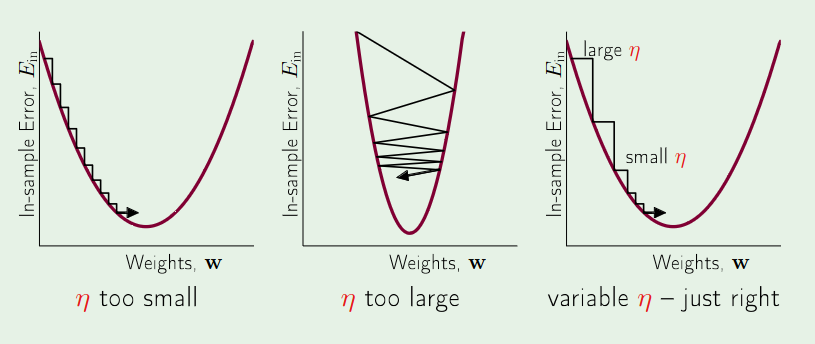
\includegraphics[width=0.5\linewidth]{Plantilla_TFG_latex//imagenes//Mat//GD/lr.png}
    \caption{Visualización de cómo afecta el \textit{learning rate} según su adecuación al problema. Imagen obtenida del curso de Caltech \footnote{https://home.work.caltech.edu/slides/slides09.pdf}, tema 9 diapositiva 21}
    \label{fig:lr}
\end{figure}

Una táctica habitual es usar una política de \textit{learning rate} que decrezca conforme avanza el entrenamiento, de manera que el algoritmo avance con pasos más grandes cuando aún está lejos del óptimo, con un objetivo explorador, y con pasos más pequeños cuando se va acercando, con un objetivo explotador, procurando una convergencia más estable. \cite{GoodFellowBook}. Otro enfoque común es también tener un vector de \textit{learning rate} en lugar de un solo escalar, teniendo un valor para cada peso del modelo. 





\subsection{Subgradientes} \label{sec:subgrad}

Con el objetivo central de calcular el gradiente es lógico pensar que necesitamos ciertas condiciones de diferenciabilidad, aunque sean mínimas, para poder calcular el gradiente que necesitamos. Podemos pensar en un modelo como una composición de la suma y producto de operaciones lineales con operaciones no lineales (funciones de activación), y componiendo ésta con la función de coste del modelo obtendríamos la función $f: X \times \Omega \times Y \rightarrow \mathbb{R^+}$, que recibe los pesos del modelo, los datos de entrada y sus etiquetas correctas para proporcionar el error del modelo. Esta es la función que necesitaríamos que fuera diferenciable. Las operaciones lineales preservan la diferenciabilidad, y la composición de funciones diferenciables es diferenciable por lo que si la función de pérdida y las funciones de activación son diferenciables, no tendremos ningún problema a la hora de calcular el gradiente.

\begin{itemize}
    \item \textbf{ECM:} $\frac{1}{N} \sum_{i=1}^N \left (y_i - \hat{y} \right ) ^2$ 

    \item \textbf{\textit{CrossEntropyLoss}:} $  - \sum_c \hat{y_c} log(\frac{e^{y_c}}{\sum_{c'=1}^C e^{y_{c'}}})$
\end{itemize}

Las funciones de coste son diferenciables de manera general, y las más comunes son por ejemplo el error cuadrático medio para problemas de regresión y \textit{CrossEntropyLoss} para problemas de clasificación. Donde $N$ es el número de datos, $\hat{y}_i$ es el valor real del dato $i$, que en ECM será un escalar, y en clasificación binaria será 0 ó 1; $y_c$ es el valor predicho por el modelo, $\hat{y}_{c}$ es la etiqueta real de la clase $c$, que valdrá 1 en caso de que el dato pertenece a la clase $c$ y 0 en caso contrario; y $y_{c}$ es el predicho por el modelo. 


Hasta el año 2010, las funciones de activación más comunes para las capas ocultas eran la función sigmoide y la tangente hiperbólica. Estas funciones son diferenciables por lo que su uso no suponía ningún problema. Sobre ese año empezaron a popularizarse las funciones de activación ReLU (Rectified Linear Unit), gracias a su simplicidad, reducción de coste computacional y su aparición en modelos ganadores de competiciones de ImageNet como AlexNet en 2012. Desde entonces esta función, junto a algunas de sus variantes que aparecen en la figura \ref{fig:3.ReLU} son ampliamente usadas y con buenos resultados. Sin embargo salta a la vista que esta función no es diferenciable.


\begin{figure}
    \centering
    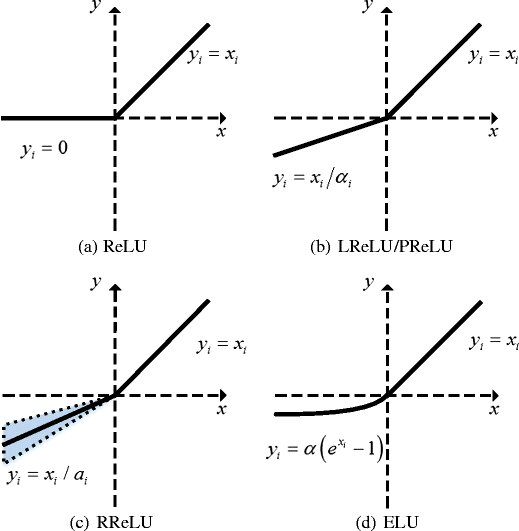
\includegraphics[width=0.5\linewidth]{3ReLU&oth.jpg}
    \caption{Función ReLU y algunas de sus variantes más usadas como funciones de activación.\footnote{https://www.researchgate.net/publication/319438080\_A\_novel\_softplus\_linear\_unit\_for\_deep\_convolutional\_neural\_networks}}
    \label{fig:3.ReLU}
\end{figure}



Vamos a presentar entonces el concepto de subgradiente junto con algunas de sus propiedades, obtenidas de \cite{convexSubgrad}, para ver que será una extensión del gradiente que nos permitirá usar el método de gradiente descendente con funciones que no sean diferenciables en algunos puntos pero que sí sean subdiferenciables.

\begin{definicion}[Subgradiente]
     Sea $A \subset \mathbb{R}^n$ y $f:A \rightarrow \mathbb{R}$, $g \in \mathbb{R}^n$ es un subgradiente de $f$ en $a \in A$ si $\forall y \in A$ se tiene:

    $$f(a)-f(y) \leq g^T(a-y)$$
    El conjunto de los subgradientes de $f$ en x se denota por $\partial f(a)$. Si existe el subgradiente de $f$ en a, decimos que $f$ es subdiferenciable en $a$.
\end{definicion}

Tenemos que comprobar que el subgradiente extiende al gradiente, es decir, que cuando existe gradiente entonces existe el subgradiente y coincide con él, y además hay funciones que no tienen el gradiente pero sí subgradiente. Vamos a definir lo que es un conjunto convexo, ya que resulta elemental tanto en esta sección como en la siguiente y usaremos este concepto para desarrollar otros a partir de él.


\begin{definicion}[Conjunto convexo]
    Un subconjunto $E$ de un espacio vectorial $X$ es convexo cuando, para cualesquiera dos puntos de $E$, el segmento que los une está contenido en $E$:

    $$x,y \in E \Rightarrow \left \{ (1-t)x + ty : t\in [0,1] \right \} \subset E$$
\end{definicion}

\begin{proposicion}[Existencia de subgradientes]
\label{prop:subgrad}
    Sea $A \subset \mathbb{R}^n$ un conjunto convexo y $f:A \rightarrow \mathbb{R}$. Si $\forall a \in A, \partial f(x) \neq \emptyset$ entonces $f$ es una función convexa. Recíprocamente, si $f$ es convexa $\forall x \in int(A)$ entonces se tiene que $\partial f(x) \neq \emptyset$. Además si $f$ es convexa y diferenciable en x se verifica que $\nabla f(x) \in \partial f(x)$.
\end{proposicion}

Para demostrar esta proposición, primero vamos a necesitar de un teorema, en el ámbito de la convexidad:

\begin{teorema}[Teorema del Hiperplano de apoyo]
    Sea $X \subset \mathbb{R}^n$ un conjunto convexo y $x_0$ un puntro de la frontera de $X$. Entonces, $\exists w \in \mathbb{R}^n, w \neq 0$ tal que
    $$\forall x \in X, \quad w^Tx \geq w^T x_0$$
\end{teorema}

\textbf{\textit{Demostración.}}
Para la primera implicación, queremos probar que $f((1-t)x+ty) \leq (1-x)f(x)+tf(y) \forall x,y \in X, \quad t \in [0,1]$, es decir, que $f$ es convexa. Partiendo de que $\forall x \in X, \quad \partial f(x) \neq \emptyset $, tomando cualquier $g \in \partial(z), \quad z \in X$ tenemos por la definición de subgradiente:

$$f(z) - f(x) \leq g^T(z-x),$$
$$f(z) - f(y) \leq g^T(z-y),$$

Para $x,y \in X$. Tomamos $z=(1-t)x + ty$ y sustituimos:
$$f((1-t)x + ty) - f(x) \leq g^T(((1-t)x + ty)-x),$$
$$f((1-t)x + ty) + g^T(x - ((1-t)x-ty) \leq f(x),$$
$$f((1-t)x + ty) + g^T(t(x-y) \leq f(x),$$

\begin{equation}\label{proof1:f(x)}
    f((1-t)x + ty) + tg^T(x-y) \leq f(x)
\end{equation}

Desarrollando en la otra desigualdad de manera análoga obtenemos

\begin{equation}\label{proof1:f(y)}
    f((1-t)x + ty) + (1-t)g^T(y-x)) \leq f(y)
\end{equation}

Ahora multiplicamos la desigualdad \ref{proof1:f(x)} por $(1-t)$ y la \ref{proof1:f(y)} por $t$, y de su suma obtenemos:

\begin{gather*}
(1-t)f(x) + tf(y) \geq \\
 (1-t)f((1-t)x+ty) + t(1-t)g^T(x-y) + tf((1-t)x+ty) + t(1-t)g^T(y-x) \\
 = f((1-t)x + ty) + t(1-t) g^T(x-y) + t(1-t)g^T(y-x)
\end{gather*}

Como se tiene que $g^T(x-y) + g^T(y-x)=0$, entonces tenemos que $(1-t)f(x) + tf(y) \geq f((1-t)x + ty), \quad \forall x,y \in X, \quad t \in [0,1]$. Por tanto $f$ es convexa, como queríamos probar.

Ahora vamos a probar que $f$ tiene algún subgradiente en $int(X)$. Definimos el epigrafo de una función $f$ como $epi(f)=\left \{ (x,t) \in X \times \mathbb{R} : t \geq f(x) \right \}$. Es obvio que f es convexa si y sólo si su epigrafo es un conjunto convexo. Vamos a aprovechar esta propidad y vamos a construir un subgradiente usando un hiperplano de apoyo al epigrafo de la función. Sea $x \in X$, claramente $(x, f(x)) \in \partial epi(f)$, y $epi(f)$ es un conjunto convexo por ser $f$ convexa. Entonces usando el Teorema del Hiperplano de Apoyo, existe $(a,b) \in \mathbb{R}^n \times \mathbb{R}$ tal que

\begin{equation}\label{proof1:epi}
    a^Tx + bf(x) \geq a^Ty + bt, \forall (y,t) \in epi(f)
\end{equation}

Reordenando tenemos

$$b(f(x)-t) \geq a^Ty - a^Tx$$

Como $t \in [f(x), + \infty [$, para que se mantenga la igualdad incluso cuando $t \rightarrow \infty$, necesitamos que $b\leq 0$. Ahora vamos a asumir que $x \in int(X)$. Entonces tomamos $\epsilon > 0$, verificando que $y=x+\epsilon a \in X$, lo que implica que $b\neq 0$, ya que si $b=0$ entonces necesariamente $a=0$. Reescribiendo \ref{proof1:epi} con $t=f(y)$ obtenemos

$$f(x) - f(y) \leq \frac{1}{|b|} a^T (x-y)$$

Por tanto $\frac{a}{|b|} \in \partial f(x)$, lo que demuestra la segunda parte de la proposición.

Para la última parte, sea $f$ una función convexa y diferenciable. Entonces por definición para $t \in [0,1]$ y $x,y \in X$

$$tf(y) + (1-t)f(x) \geq f((1-t)x + ty)$$

$$f(y) \geq \frac{f((1-t)x + ty) - (1-t)f(x)}{t}$$

$$= f(x) + \frac{f(x + t(y-x)) - f(x)}{t}$$

$$ \xrightarrow[t \rightarrow 0]{} \quad f(x) + \nabla f(x)^T (y-x)$$

Lo que demuestra que $\nabla f(x) \in \partial f(x)$


\begin{flushright}
    $\square$
\end{flushright} 




Necesitamos también un comportamiento similar al de las funciones diferenciables, en particular necesitamos que las funciones subdiferenciables se preserven a través de las operaciones de suma, multiplicación por escalares y composición.

\begin{enumerate}

	\item \textbf{Multiplicación escalar no negativa}: $\partial (af) = a \cdot \partial f , a\geq0$
	
	\item \textbf{Suma}: $\partial (f_1+f_2) = \partial f_1 + \partial f_2$
	
	\item \textbf{Composición afín}: Si $g(x)=f(Ax + b) \Rightarrow \partial g(x)= A^T \partial f(Ax+b)$
	
	%\item \textbf{Máximo finito}: Si $f(x) = max_{i=1,...,n} f_i(x)$ entonces
	 %$$\partial f(x) = conv \left ( \underset{i: f_i(x)=f(x)}{\cup} \partial f_i(x) \right )$$
	
	%\item \textbf{Máximo general}: Si $f(x) = max_{s  \in S} f_s(x)$ entonces 
	%$$  \overline{\left \{  conv \left ( \underset{s:f_s(x)=f(x)}{\cup} \partial f_s(x) \right )    \right \}  \subseteq \partial f(x)}$$

\end{enumerate}

Tenemos entonces que el subgradiente es una extensión del gradiente en aquellos puntos que no son diferenciables. Por ello podríamos decir que existe el método de descenso de subgradiente, que permite usar funciones que no son diferenciables en todos los puntos, y que se usa de manera implícita en el momento en el que en un modelo se usan funciones ReLU, por ejemplo. Conviene destacar esta diferencia para no perder la rigurosidad, aunque solo sea una formalidad, ya que realmente no se hacen diferencias entre uno y otro método, así que nos seguiremos refiriendo al método de descenso de gradiente aunque estemos trabajando con subgradientes. En \cite{ReLuat0} se analiza la elección del valor que toma el subgradiente en el punto $x=0$ y se ve su influencia, que no es poca, en la ejecución del algoritmo, y se concluye que el valor 0 es el que ofrece mejor robustez de manera general.

\begin{ejemplo}[Subgradiente de la función ReLU]\label{ej:RELUsub}
     La función ReLU es continua en todo el dominio y diferenciable en $]-\infty,0[ \cup ]0,\infty[$. Su subgradiente es el siguiente:

    $$ \nabla ReLU(x)=\left\{\begin{matrix}
1, \quad si \quad x \in ]0,\infty[ \\
c \in [0,1] \quad si \quad x=0\\
0 \quad si \quad x \in ]-\infty,0[
\end{matrix}\right.$$
\end{ejemplo}




\subsection{Convergencia} \label{sec:convergencia}

La convergencia es un factor crucial en el algoritmo de gradiente descendente. Al tratarse de un algoritmo de optimización iterativo, iremos buscando el mínimo global de la función de coste en varios pasos, o en su defecto un mínimo local que nos ofrezca una solución subóptima. El algoritmo se mueve hacia puntos de menor gradiente por lo que convergerá a puntos donde el gradiente sea 0. Un factor clave para la convergencia será el hecho de que la función de pérdida sea o no una función convexa.




\begin{definicion}[Función convexa]
    Sea $E \subset \mathbb{R}^n$ un conjunto convexo no vacío y sea $f:E \rightarrow \mathbb{R}$, $f$ es una función convexa en $E$ si, y solo si:

    $$f(tx + (1-t)y) \leq tf(x) + (1-t) f(y), \quad \forall t \in [0,1], \forall x,y \in E$$
\end{definicion}


En caso de que la función de coste sea convexa sólo existirá un mínimo y será global, por lo que no tenemos que preocuparnos de si el algoritmo se queda estancado en un mínimo local, ya que si converge tenemos la solución óptima. Además en este caso el análisis de la convergencia resulta mucho más sencillo, y por eso encontramos más resultados teóricos y más fuertes que en el caso contrario. Desgraciadamente la situación normal es que la función de coste no sea convexa, y de hecho comprobar que una función sea convexa se trata de un problema NP-Hard \cite{Ahmadi_2011_NP_Convex}, por lo que en la práctia normalmente no realizamos el análisis teórico de la función y la convergencia previo al entrenamiento del modelo. En caso que no sea convexa, podemos converger hacia un punto crítico que no sea un mínimo global, con lo cual el algoritmo parará y puede que hallamos llegado a una solución que aunque sea subóptima no sea lo suficientemente buena.



\subsubsection{Resultados teóricos para la convergencia del gradiente descendente}

Los desarrollos teóricos sobre la convergencia del algoritmo de descenso del gradiente son muchos y variados. Los principales inconvenientes para el desarrollo de un marco teórico que sea útil en la práctica son:

\begin{itemize}

    \item No existen resultados generales que nos permitan conocer el comportamiento de la convergencia del algoritmo en el problema que estemos tratando con un coste asequible. Los resultados son muy específicos y dependen de la función de coste, el valor de los hiperparámetros y la versión del algoritmo de gradiente descendente que estemos utilizando.

    \item El estudio teórico de la función de coste es muy complejo y requiere tanto tiempo como recursos computacionales. Por lo tanto la tendencia a nivel experimental es invertir esos recursos en el entrenamiento, ya que ofrece mejores resultados en relación coste/beneficio de manera genérica que el estudio teórico de los elementos del algoritmo. Además es un procedimiento genérico aplicable en cualquier problema, por lo que resulta más sencillo.

    \item La mayoría de resultados teóricos aprovechables son basados en el gradiente descendente original (BGD), ya que cuando introducimos el ruido que genera la aproximación del cálculo del gradiente en sus variantes SGD y MBGD se complica el desarrollo teórico. Los resultados que aparecen a continuación son, a menos que se especifique lo contrario, resultados para BGD.
   
\end{itemize}


En el caso que la función de coste sea convexa tenemos un caso más sencillo de analizar, principalmente debido a la curvatura que tienen las funciones convexas y al hecho de que cualquier punto crítico será un mínimo global.

\begin{comment}
			
			\begin{proposicion}
			    Sea $f:\mathbb{R}^n \rightarrow \mathbb{R}$ una función de coste que es convexa con su gradiente $\nabla f$ Lipschitz continuo, con constante de Lipschitz $L>0$. Si el \textit{learning rate} $\eta$ se elige de manera que $0<\eta<\frac{2}{L}$, entonces el algoritmo de gradiente descendente converge a un punto $x_m$ que es mínimo global de la función $f$ \cite{murphy2022probabilistic}
			\end{proposicion}
			
			Esto nos asegura que seleccionando un \textit{learning rate} adecuado el algoritmo converge a un mínimo global, que es lo que buscamos. Como en la práctica es demasiado complejo encontrar la constante de Lipschitz, podemos seleccionar un valor suficientemente cercano a 0 para asegurarnos la convergencia y luego ir probando a aumentarlo poco a poco para obtener una velocidad de convergencia adecuada.
			
			Si tenemos una función de coste que, no solo es convexa, sino que es fuertemente convexa, entonces además de la convergencia a un mínimo global tenemos asegurada la velocidad de la convergencia de éste:
			
			
			\begin{proposicion}
			    Sea $f:\mathbb{R}^n \rightarrow \mathbb{R}$ una función de coste que es fuertemente convexa con su gradiente $\nabla f$ Lipschitz continuo, con constante de Lipschitz $L>0$. Entonces el algoritmo de gradiente descendente converge a un punto $x_m$ que es mínimo global de la función $f$, y además existe una constante $\rho \in [0,1]$ que verifica $\| x_k - x_m \| \leq \rho^k \| x_0 - x_m\|$. Es decir, la convergencia es lineal \cite{ConvexOp}.     
			\end{proposicion}
			
			Aunque el orden lineal no parezca demasiado bueno, en la anterior proposición ni siquiera la teníamos asegurada. En la práctica cuando usamos optimizadores generalmente conseguimos mayor orden de convergencia aunque no lo tenemos asegurado. Cabe recordar que, aunque usemos terminología referente a métodos iterativos, el gradiente descendente no es un método numérico.
			
			
			Ahora tenemos un resultado más general, no haciendo uso de funciones convexas. Este es el caso más común.

\end{comment}



\begin{teorema}[Convergencia para funciones convexas]\label{proof:gdconvex}
    Suponemos $f$ una función convexa y diferenciable, con su gradiente Lipschitz continuo con constante $L>0$, teniendo que $\| \nabla f(x) - \nabla f(y) \|_2 \leq L \|x-y\|_2 \quad \forall x, y$. Si ejecutamos el algoritmo de gradiente descendente $k$ iteraciones con un $\eta<1/L$ constante, el error disminuirá tras cada iteración, llegando a una solución $f^{(k)}$ que satisface la siguiente ecuación:

    $$f(x^{(k)})-f(x^*) \leq \frac{\|x^{(0)}-x^* \|^2_2}{2\eta k}$$

    Donde $x^*$ es el mínimo global de la función de error. 
\end{teorema}

\vspace{1cm}

\begin{flushleft}
   \textbf{\textit{Demostración.}}
\end{flushleft} 



En el teorema anterior $x \in \mathbb{R}^n$ son los pesos del modelo, y suponemos que el conjunto de datos con el que entrenamos es constante, por lo tanto el error del modelo, $f(x)$, sólo dependerá de los parámetros $x$.

Como $\nabla f$ es Lipschitz continuo con constante $L$ entonces $\nabla ^2 f(x) \preceq LI$, donde $I$ es la matriz identidad. Equivalentemente esto significa que $\nabla ^2 f(x) -LI$ es una matriz semidefinida negativa. Ahora hacemos un desarrollo cuadrático de $f$ alrededor de $f(x)$ para obtener:

\begin{gather*}
    f(y) \leq f(x) + \nabla f(x)^T (y-x) +\frac{1}{2}\nabla^2 f(x) \|y-x\|^2_2  \\
    \leq f(x) + \nabla f(x)^T(y-x) + \frac{1}{2}L \|y - x \|^2_2
\end{gather*}

Consideramos ahora $y$ como la actualización de los pesos del gradiente descendente, $y=x - \eta \nabla f(x)=x^+$. 


\begin{gather*}
    f(x^+) \leq f(x) + \nabla f(x)^T(x^+-x) + \frac{1}{2}L \|x^+ - x \|^2_2 \\
    = f(x) + \nabla f(x)^T(x - \eta \nabla f(x) -x) + \frac{1}{2}L \|x - \eta \nabla f(x) - x \|^2_2 \\
    = f(x) - \eta \nabla f(x)^T \nabla f(x) + \frac{1}{2} L \| \eta \nabla f(x) \|^2_2 \\
    = f(x) - \eta \| \nabla f(x) \|^2_2 + \frac{1}{2} L \eta^2 \| \nabla \|^2_2 \\
    = f(x) - (1- \frac{1}{2}L \eta) \eta \| \nabla f(x) \|^2_2
\end{gather*}

Usamos $\eta \leq \frac{1}{L}$ para ver que $-(1-\frac{1}{2}L \eta)= \frac{1}{2} L \eta - 1 \leq \frac{1}{2} L (\frac{1}{L}) - 1 = \frac{1}{2} - 1 = -\frac{1}{2}$, y sustituyendo esta expresión en la desigualdad anterior obtenemos 

\begin{equation}\label{eq:gdproof1}
	f(x^+) \leq f(x) - \frac{1}{2} \eta \| \nabla f(x) \|^2_2 
\end{equation}

Esta última desigualdad se traduce en que tras cada iteración del algoritmo del descenso de gradiente el valor del error del modelo es estrictamente decreciente, ya que el valor de $\frac{1}{2} \eta \| \nabla f(x) \|^2_2$ siempre es mayor que 0 a no ser que $\nabla f(x)=0$, en cuyo caso habremos encontrado el óptimo. 

Ahora vamos a acotar el valor del error en la siguiente iteración, $f(x^+)$, en términos del valor óptimo de error $f(x^*)$. Como $f$ es una función convexa se tiene

\begin{align*}
    f(x^*) \geq f(x) + \nabla f(x) ^T (x^* - x) \\
    f(x) \leq f(x^*) + \nabla f(x)^T (x-x^*)
\end{align*}

La segunda desigualdad se deduce de la primera de manera inmediata. Sustituyendo esa segunda desigualdad en \ref{eq:gdproof1} obtenemos

\begin{gather*}
    f(x^+) \leq f(x^*) + \nabla f(x)^T (x-x^*) - \frac{\eta}{2} \| \nabla f(x) \| ^2_2 \\ 
    f(x^+) - f(x^*) \leq  \frac{1}{2\eta}  \left ( 2 \eta \nabla f(x)^T (x-x^*) - \eta ^2 \| \nabla f(x) \| ^2_2 \right ) \\ 
    f(x^+) - f(x^*) \leq  \frac{1}{2\eta}  \left ( 2 \eta \nabla f(x)^T (x-x^*) - \eta ^2 \| \nabla f(x) \| ^2_2 - \| x - x^* \|^2_2 + \| x - x^* \|^2_2 \right )    
\end{gather*}

Como $  2 \eta \nabla f(x)^T (x-x^*) - \eta ^2 \| \nabla f(x) \| ^2_2 - \| x - x^* \|^2_2 = \| x - \eta \nabla f(x) - x^* \|^2_2 $, se tiene que

$$ f(x^+) - f(x^*) \leq  \frac{1}{2\eta}  \left ( \| x - x^+ \|^2_2 -  \| x - \eta \nabla f(x) - x^* \|^2_2 \right ) $$

Usamos ahora la definición de $x^+$ en esta última desigualdad

$$ f(x^+) - f(x^*) \leq  \frac{1}{2\eta}  \left ( \| x - x^+ \|^2_2 -  \| x^+ - x^* \|^2_2 \right ) $$

Hacemos la sumatoria sobre las $k$ primeras iteraciones y tenemos

\begin{gather*}
    \sum^k_{i=1} \left ( fx^{(i)} - f(x^*) \right ) \leq \sum^k_{i=1} \frac{1}{2\eta}  \left ( \| x^{(i-1)} - x^+ \|^2_2 -  \| x^{(i)} - x^* \|^2_2 \right ) \\ 
    \frac{1}{2\eta}  \left ( \| x^{(0)} - x^+ \|^2_2 -  \| x^{(k)} - x^* \|^2_2 \right ) \\ 
    \leq \frac{1}{2\eta}  \left ( \| x^{(i-1)} - x^+ \|^2_2 \right )  
\end{gather*}

El sumatorio de la derecha ha desaparecido ya que es una serie telescópica. Usando que $f$ decrece con cada iteración, e introduciendo la anterior desigualdad, finalmente llegamos a donde queríamos:

$$f(x^{(k)} - f(x^*) \leq \frac{1}{k} \sum ^k _{i=1} \left ( f(x^{(i)} - f(x^*) \right ) \leq \frac{\|x^{(0)}-x^* \|^2_2}{2\eta k} $$


\begin{flushright}
    $\square$
\end{flushright} 


Este teorema nos garantiza que bajo las condiciones supuestas el algoritmo del gradiente descendente converge y además lo hace con ratio de convergencia de $O(1/k)$. Es un resultado teórico muy fuerte que por desgracia no puede usarse en la práctica en la gran mayoría de casos: la constante de Lipschitz $L$ es computacionalmente costosa de calcular, por lo que se usan aproximaciones experimentales para el $\eta$, además en muy contadas ocasiones la función de error con la que trabajamos es convexa, y tampoco es sencilla de calcular por lo que directamente no se comprueba si lo es o no lo es, y directamente la suponemos no convexa. 

Podemos obtener un resultado mucho más práctico, ya que es para SGD y MBGD y además con condiciones más relajadas. Usando la teoría de algoritmos aproximados estocásticos, en concreto el teorema de Robbins-Siegmund tenemos que bajo las siguientes condiciones, cuando la función es convexa se tiene la convergencia casi segura al mínimo global y cuando no lo es hay convergencia casi segura a un punto crítico. Esto nos da un criterio sencillo para la convergencia, y que no depende de parámetros como la constante de Lipschitz que son complejos de computar.


\begin{proposicion}[Convergencia para SGD]
    Sea ${x_k}$ la secuencia generada por el algoritmo de SGD, sea $f$ la función de coste del modelo y sea $\eta_k$ el valor del \textit{learning rate} en la iteración $k$. Si la sucesión ${\eta_k}$ satisface $\sum_{k=1}^\infty \eta_k = \infty$ y también $\sum_{k=1}^\infty \eta_k ^2 < \infty$  entonces $\lim_{k\rightarrow\infty} \| \nabla f(x_k) \| =0$. Es decir, el algoritmo converge hacia un punto crítico de la función.% \cite{GoodFellowBook}.
\end{proposicion}

Aunque la complejidad de la demostración se escapa al alcance de este TFG, ya que sería necesario demasiadas definicones y resultados previos, en la página 33 de \cite{RobbinSiegmund} \footnote{El original 'A convergence theorem for non negative almost supermartingales and some applications' es de pago y no puedo acceder} podemos encontrar el enunciado y demostración del teorema de Robbins-Siegmund. En \cite{RobbinSiegmundtoSGD} podemos observar su uso para la demostracion de la convergencia de SGD. Hay que remarcar que, aunque la demostración de la convergencia se realiza en supuesto de función convexa a un mínimo global, se puede tomar una restricción local de la función de manera que esta sea convexa y se alcance un punto crítico.



%TODO: podría añadir algunos resultados de aquí: https://arxiv.org/pdf/1405.4980, como el de funciones fuertenemente convexas. También podria meter cierta equivalencia entre GD y SGD.



\subsubsection{Problemas en la convergencia}


En el teorema anterior tenemos asegurada la convergencia a un mínimo, sin embargo en el segundo solo nos garantizamos llegar a un punto crítico, ni siquiera a un mínimo local. Encontramos aquí el mayor problema del algoritmo del gradiente descendente: la convergencia prematura en puntos con gradiente muy cercano a cero. 

Cuando el algoritmo se aproxima a un punto crítico, la magnitud del gradiente se aproxima a cero, y teniendo en cuenta la regla de actualización de los pesos, $W_{t+1}=W_t - \eta \nabla C(W)$, tenemos por tanto que $W_{t+1} - W_t \approx 0$. Es decir que las modificaciones de los pesos con las actualizaciones serán prácticamente nulas, haciendo que el algoritmo se pare o que progrese de manera muy lenta cerca de estos puntos, lo que en un primer momento podría aparentar una falsa convergencia en regiones planas por ejemplo. 

Los puntos críticos más comunes son los puntos de silla, que definimos como un punto $x_s$ de una función $f(x)$ verifica que $\nabla f(x_s)=0$ pero $x_s$ no es ni un mínimo local ni un máximo local. En $x_s$ la matriz Hessiana de $f$, $\nabla^2 f(x_s)$ tiene valores propios tanto positivos como negativos, lo que indica que la función $f$ se curva hacia abajo en unas direcciones y hacia arriba en otras en el punto $x_s$.

En espacios de alta dimensionalidad, que son comunes en las redes neuronales, la probabilidad de encontrar puntos de silla es mucho mayor que la de encontrar máximos y minímos locales. Para una función $f:\mathbb{R}^n \rightarrow \mathbb{R}$, el número de puntos de silla normalmente crece exponencialmente con respecto a la dimensión $n$. Esto se debe a que la probabilidad de encontrar valores propios de ambos signos en la matriz Hessiana aumenta con la dimensionalidad del espacio de parámetros \cite{dauphin2014SaddlePoints}. 

La manera de solventarlos es utilizar modificaciones en el algoritmo de gradiente descendente que proporcionan mejores propiedades a su comportamiento, ya que las estrategias de SGD y MBGD ofrecen una pequeña pero insuficiente solución a este problema. Al calcular el gradiente mediante una aproximación con un subconjunto de los datos, se introduce un ruido $\epsilon$ en su cálculo con lo que $W_{t+1} - W_t \approx \epsilon$, que puede servir para conseguir escapar de ese punto de silla. Estas modificaciones se denominan optimizadores y a diferencia de las versiones vistas en la sección \ref{sec:estrategias}, que variaban solo en la cantidad de datos usados para calcular el gradiente, estos optimizadores cambian la regla de actualización de los pesos añadiendo nuevos cálculos, hiperparámetros y estrategias para conseguir que el algoritmo mejore en estabilidad, robustez y velocidad de convergencia.


Existen otros problemas como la explosión o el desvanecimiento de gradiente, pero están ligados a BP como herramienta para calcularlo, por lo que se abordarán en la sección siguiente junto a la inicialización de pesos del modelo, que es la manera principal de superar estos problemas.







\section{\textit{Backpropagation}}
Ya conocemos el algoritmo de aprendizaje del gradiente descendente y, en esta sección, abordaremos el algoritmo BP, que, como hemos mencionado, es el método más utilizado para calcular el gradiente durante el entrenamiento de un modelo. Cuando se desean obtener las predicciones de una red neuronal para un conjunto de datos de entrada, la información fluye desde la capa de entrada $x$, atravesando las capas ocultas hasta generar una salida $o$, que si es evaluada con la función de coste $C$ produce un escalar $E$ que representa el error del modelo. Este proceso, refiriéndonos a cómo se transmite la información entre capas, se conoce como \textbf{propagación hacia delante} (\textit{forward propagation}).

Para calcular el gradiente de la función de coste con respecto a los pesos del modelo, es necesario que la información fluya en sentido inverso, es decir, que el error $E$ se propague desde la salida, pasando por las capas ocultas, hasta la capa de entrada $x$. Este proceso se conoce como \textbf{propagación hacia atrás} (\textit{backpropagation}). \textbf{El algoritmo de BP toma su nombre de aquí} ya que durante su aplicación necesitamos que la información se propage hacia atrás. Si bien, \textbf{no se trata del mismo concepto}, ya que podemos propagar la información hacia atrás sin necesidad de calcular el gradiente, en cuyo caso no estaríamos aplicando BP.






\subsection{Diferenciación automática}

\textbf{El algoritmo de BP se implementa en la práctica a través de la diferenciación automática} \cite{AutomaticDiff}, que es un algoritmo más general para calcular derivadas y que engloba a BP. Se fundamenta en descomponer las funciones en una secuencia de operaciones fundamentales para calcular sus derivadas a través de la regla de la cadena, haciendo este cómputo muy eficiente. Por ello se distingue de la diferenciación simbólica, que manipula las expresiones matemáticas para encontrar derivadas, y de la diferenciación numérica, que calcula las derivadas a través de aproximaciones con diferencias finitas. Esta es la implementación que se usa en las librerías de aprendizaje automático más usadas, como TensorFlow 2\footnote{\url{https://www.tensorflow.org/}} y PyTorch\footnote{\url{https://pytorch.org/}}.

En la diferenciación automática existen dos estrategias para calcular un vector gradiente o una matriz jacobiana: diferenciación hacia delante y diferenciación hacia atrás. Su distinción reside principalmente en si realizamos multiplicaciones de un vector por un jacobiano (hacia atrás) o de un jacobiano por un vector (hacia delante). La elección dependerá de las dimensiones de la matriz jacobiana que queramos calcular, en otras palabras, debemos comparar la dimensión de la entrada y de la salida del modelo. Si la dimensión de entrada es mayor que la de salida, el cálculo de la matriz jacobiana requiere menos operaciones cuando se emplea la diferenciación hacia atrás; por el contrario, si la dimensión de salida es mayor que la de entrada, resulta más eficiente utilizar la diferenciación hacia adelante.. 

Debido a la estructura general de una red neuronal donde la dimensión de la entrada es mucho mayor que la de la salida, resulta más eficiente calcular el gradiente con la diferenciación hacia atrás, y esto es lo que entendemos como el algoritmo de BP: la información se propaga hacia atrás en el modelo mientras que se usa la diferenciación hacia atrás con el objetivo de calcular el gradiente del error del modelo con respecto a sus pesos. Si utilizáramos la diferenciación hacia delante, aunque estuviéramos propagando la información hacia atrás no estaríamos usando el algoritmo de BP, y además el cálculo resultaría mucho más ineficiente. Se suele afirmar que el algoritmo de BP es una aplicación concreta de la diferenciación automática hecha a medida para el entrenamiento de redes neuronales.


Vamos a explorar el algoritmo de BP de manera progresiva: en primer lugar veremos la diferenciación hacia delante y hacia atrás, viendo por qué es más eficiente usar la segunda y acotando este algoritmo general para llegar al algoritmo de BP, para lo que veremos cómo calcular la matriz jacobiana de la salida de un perceptrón multicapa (MLP, por sus siglas en inglés) respecto a la entrada, en una situación que no será de entrenamiento, ya que no habrá parámetros entrenables, pero nos servirá para ilustrar el funcionamiento de BP. Luego veremos cómo obtenemos el gradiente del error con respecto a los pesos de cada capa usando el algoritmo de BP en un MLP con parámetros entrenables, concretando con ejemplos para las capas más comúnmente utilizadas. Finalmente vamos a generalizar este concepto hacia modelos más abstractos usando grafos dirigidos acíclicos. 


Los MLP son un tipo de red neuronal, divididos en capas compuestas de nodos llamados neuronas, donde cada nodo de cada capa está conectado con todos los nodos de la capa siguiente. Son usados principalmente con conjuntos de entrenamiento tabulares, es decir aquellos que sus datos tienen formato de tabla. Usaremos esta arquitectura para realizar el desarrollo teórico ya que es más sencilla conceptualmente y facilita la notación. 

\subsection{Diferenciación hacia delante vs hacia atrás}


Definimos nuestro modelo como $f: \mathbb{R}^n \rightarrow \mathbb{R}^m$, $o=f(x)$ con $x \in \mathbb{R}^n$  y $o \in \mathbb{R}^m$. Asumimos que $f$ es una composición de funciones:

$$f=f_k \circ f_{k-1} \circ \cdots \circ f_2 \circ f_1.$$

Donde $k-1$ es el número de capas ocultas del MLP y $k+1$ el total de capas. Cada función $f_i$ representa el cálculo que se realiza en la capa $i$-ésima. Se tiene para $i \in \left \{ 1,\ldots,k \right \}$


$$f_i: \mathbb{R}^{m_i} \rightarrow \mathbb{R}^{m_{i+1}}$$

$$f_i(x_i)=x_{i+1}$$

Donde la entrada del modelo viene representada en la primera capa, $x=x_1$. Además se tiene que $m_1=n, m_{k+1}=m, x_{k+1}=o$. Para obtener la predicción del modelo, $o=f(x)=f_k(x_k)$, necesitamos calcular el resultado de todas las capas intermedias $x_{i+1}=f_i(x_i)$. 

Podemos ver que la matriz jacobiana de la salida con respecto a la entrada $J_f(x) \in  \mathbb{R}^{m\times n}$ puede ser calculada usando la regla de la cadena . Esto nos va a servir para ilustrar las diferencias entre la diferenciación hacia atrás y hacia delante


\begin{equation*}
	J_f(x) = J_{f_k}(x_k) J_{f_{k-1}}(x_{k-1}) \cdots J_{f_2}(x_2) J_{f_1}(x_1).
\end{equation*}



%&= \frac{\partial o}{\partial x} = \frac{\partial o}{\partial x_k} \frac{\partial x_k}{\partial x_{k-1}} \cdots \frac{\partial x_3}{\partial x_2} \frac{\partial x_2}{\partial x_1} \\	
	%&=\frac{\partial f_k(x_k)}{\partial x_k} \frac{\partial f_{k-1}(x_{k-1})}{\partial x_{k-1}} \cdots \frac{\partial f_2(x_2)}{\partial x_2} \frac{\partial f_1(x_1)}{\partial x_1} \\	
	%&
Se discute ahora cómo calcular el jacobiano $J_f(x)$ de manera eficiente. Recordamos\footnote{Aquí interpretamos los vectores gradiente y derivada parcial como vectores columna} que 

\begin{align*}
	J_f(x_1)&=
	\begin{pmatrix}
	\frac{\partial f_1}{\partial x_1} & \cdots & \frac{\partial f_1}{\partial x_n} \\	
	\vdots & \ddots & \vdots \\
	\frac{\partial f_m}{\partial x_1} & \cdots & \frac{\partial f_m}{\partial x_n} 
	\end{pmatrix} \\
	&= 
	\begin{pmatrix}
	 \nabla f_1(x)^T\\
	 \vdots \\
	 \nabla f_m(x)^T \\
	\end{pmatrix}=
	\begin{pmatrix}
	     \frac{\partial f}{\partial x_1}, \ldots, \frac{\partial f}{\partial x_n}
	\end{pmatrix} \in \mathbb{R}^{m \times n}.
\end{align*}





Donde $\nabla f_i(x) ^T \in \mathbb{R}^{1 \times n} $ es la fila $i$-ésima y $\frac{\partial f}{\partial x_j} \in \mathbb{R}^m$ es la columna $j$-ésima de la matriz jacobiana , para $i=1,\ldots,m$ y $j=1,\ldots,n$.

Podemos extraer la fila $i$-ésima del jacobiano usando un producto vector-jacobiano (PVJ) de la forma $e_i^T J_f(x)$, donde $e_i \in \mathbb{R}^m$ es el vector de la base canónica. De manera análoga se puede extraer la columna $j$-ésima de $J_f(x)$ usando un producto jacobiano-vector (PJV) de la forma $J_f(x)e_j$, donde $e_j \in \mathbb{R}^n$. Se tiene entonces que el cálculo de la matriz jacobiana $J_f(x)$ equivale a $n$ PJV o $m$ PVJ. 


Para construir el jacobiano a partir de operaciones PJV o PVJ, podemos suponer que el cálculo del gradiente de $f_i(x)$ tiene el mismo coste computacional que el cálculo de la derivada parcial de $f$ con respecto de alguna de las variables $x_j$. Por tanto la forma de cálculo más eficiente de la matriz jacobiana depende de qué valor es mayor: si $n$ o $m$.



Si $n\leq m$ será más eficiente construir el jacobiano $J_f(x)$ usando PJV de derecha a izquierda.

$$J_f(x)v=J_{f_k}(x_k) \cdots J_{f_2}(x_2) J_{f_1}(x_1) v.$$

Donde $J_{f_k}(x_k)$ tiene tamaño $m \times m_{k-1}$, $J_{f_i}(x_i)$ tiene tamaño $m_i \times m_{i-1}$ para $i \in {2,\ldots,k-1}$ y $J_{f_1}(x_1)$ tiene tamaño $m_1 \times n$ mientras que el vector columna $v$ será $n \times 1$. Esta multiplicación se puede calcular usando el agoritmo de diferenciación hacia delante definido en el Algoritmo \ref{alg:fowdiff}.

\begin{algorithm}[H]
\caption{Diferenciación hacia delante}
\label{alg:fowdiff}
    \begin{algorithmic}
        \State $x_1 := x$
        \For{$j \in \left \{ 1,\ldots,n\right \}$}
            \State $v_j := e_j \in \mathbb{R}^n$
        \EndFor
        \For{$i \in \left \{ 1,\ldots,k \right \}$}
            \State $x_{i+1}:=f_i(x_i)$
            \For{$j \in \left \{ 1,\ldots,n\right \}$}
                \State $v_j:= J_{f_i}(x_i)v_j$
            \EndFor
        \EndFor 

        
         \Return $o=x_{k+1}, \left (v_1, v_2, \ldots, v_n \right )$
        
    \end{algorithmic}
\end{algorithm}

Donde los elementos $v_j, j \in \left \{1,\ldots,n \right \}$ de la matriz fila $v$ se corresponden con las derivadas parciales de la función del MLP respecto a la entrada de la capa $j$, es decir la columna $j$-ésima de la matriz jacobiana, $v_j=\frac{\partial f}{\partial x_j}$. 

Si $n\geq m$ es más eficiente calcular $J_f(x)$ para cada fila $i=1,\ldots,m$ usando PVJ de izquierda a derecha. La multiplicación izquierda con un vector fila $u^T$ es 

$$u^TJ_f(x)=u^TJ_{f_k}(x_k) \cdots J_{f_2}(x_2) J_{f_1}(x_1).$$

Donde $u^T$ tiene tamaño $1 \times m$,  $J_{f_k}(x_k)$ tiene tamaño $m \times m_{k-1}$, $J_{f_i}(x_i)$ tiene tamaño $m_i \times m_{i-1}$ para $i \in {2,\ldots,k-1}$ y $J_{f_1}(x_1)$ tiene tamaño $m_1 \times n$. Esto puede calcularse usando la diferenciación hacia atrás (ver Algoritmo \ref{alg:backdif}).

 


\begin{algorithm}
\caption{Diferenciación en modo reverso}
\label{alg:backdif}
    \begin{algorithmic}
        \State $x_1:=x$
        \For{$k \in \left \{1,\ldots,K \right \}$}
            \State $x_{k+1} = f_k(x_k)$
        \EndFor
        \For{$i \in \left \{1,\ldots,m \right \}$}
            \State $u_i:=e_i \in \mathbb{R}^m$
        \EndFor 
        \For{$k \in \left \{ K,\ldots,1 \right \}$}
            \For{$i \in \left \{ 1,\ldots,m \right \}$}
                \State $u_i^T:= u_i^T J_{f_k}(x_k)$
            \EndFor
        \EndFor 

        \Return $o=x_{k+1}, \left ( u_1^T, u_2^T, \ldots, u_m^T \right )$
    \end{algorithmic}
\end{algorithm}

Donde los elementos $u_i^T$ se corresponden con el gradiente de la función $f_i$, $u_i^T=\nabla f_i(x)^T$, es decir la fila $i$-ésima de la matriz jacobiana. Asumimos que $m=1$ ya que la salida de la función de error del modelo es un escalar, y que $n=m_i$ $i \in \left \{2,\ldots, k-1 \right \}$; entonces el coste de computar el jacobiano usando la diferenciación hacia atrás es $O(n^2)$. Este algoritmo aplicado al cálculo del gradiente del error del modelo con respecto a los pesos, propagando la información hacia atrás y con el objetivo de usar gradiente descendente, es lo que conocemos como BP.  Podemos ver una representación gráfica de ambos modos de diferenciación en la Figura \ref{fig:bp_1}.

\begin{figure}
    \centering
    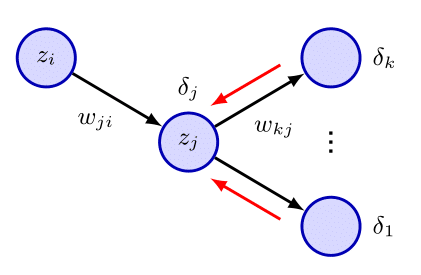
\includegraphics[width=0.7\linewidth]{Plantilla_TFG_latex/imagenes/Mat/Definicion/bp_1.png}
    \caption[Cálculo del error para una unidad oculta ilustando la propagación hacia delante y la propagación hacia atrás del error]{Cálculo del error $\delta_j$ para la unidad oculta $j$ mediante la propagación hacia atrás del error ($\delta$). En la imagen, el nodo $z_j$ representa una neurona en una capa oculta de la red neuronal. Esta neurona recibe una entrada desde otra neurona $z_i$ con un peso sináptico asociado $w_{ji}$ (indicado por la flecha negra). A su vez, la neurona $z_j$ está conectada a varias neuronas $z_k$ en la siguiente capa, con pesos $w_{kj}$. Durante la propagación hacia adelante (flechas negras), la información fluye desde las entradas hacia las salidas de la red. Durante la propagación hacia atrás del error (flechas rojas), los valores de error $\delta_k$ de las neuronas de la capa siguiente se propagan hacia atrás para calcular $\delta_j$, lo que permite ajustar los pesos en función del gradiente del error. Imagen obtenida de \cite{bishop2023learning}.}
    \label{fig:bp_1}
\end{figure}

Con la notación que estamos empleando, cuando $m=1$ el gradiente $\nabla f(x)$ tiene la misma dimensión que $x$. Por tanto es un vector columna mientras que $J_f(x)$ es un vector fila, por lo que técnicamente se tiene que $\nabla f(x)= J_f(x)^T$. Es de vital importancia aclarar esto ya que es el caso en el que nos situamos cuando usamos BP. La dimensión de salida siempre es uno, ya que calculamos la matriz jacobiana de la función de error del modelo con respecto a los pesos, con lo que será un vector gradiente de dimensión igual a la dimensión de los pesos del modelo. La predicción del modelo puede tener dimensión 1 en tareas de regresión, o una dimensión mayor para tareas de clasificación, aunque de manera general no suele ser mayor de 100. La función de error del modelo siempre tendrá como imagen un valor real.


Hemos demostrado que, para el cálculo de una matriz jacobiana, la diferenciación hacia adelante es más eficiente cuando la dimensión de la entrada es menor que la de la salida, mientras que la diferenciación hacia atrás resulta más adecuada cuando la dimensión de la salida es menor que la de la entrada. Dado que en las redes neuronales y los problemas en los que se aplican la dimensión de salida es, por lo general, considerablemente menor que la de entrada, la diferenciación hacia atrás es la opción más eficiente en estos casos.




\subsection{\textit{Backpropagation} en perceptrones multicapa}


En la sección anterior, analizamos un modelo que no tenía parámetros entrenables. Ahora, utilizaremos un modelo que sí los tiene y \textbf{exploraremos cómo calcular el gradiente de la función de coste con respecto a esos parámetros entrenables}. Los parámetros son valores reales y tienen la forma $W= W_1 \times W_2 \times \cdots \times W_k \subset \Omega$, con $W_i \in \mathbb{R}^{n_i \times n_{i+1}}$ donde $n_i$ es el número de neuronas de la $i$-ésima capa. El modelo que tendríamos añadiendo los pesos es $f: \mathbb{R}^n \times \Omega \rightarrow \mathbb{R}^m$, $o=f(x,W)$ con $x \in \mathbb{R}^n$  y $o \in \mathbb{R}^m$. Donde las funciones de cada capa son de la forma $f_i(x_i, W_i)= \sigma_i(W_ix_i)=x_{i+1}$ donde $\sigma_i$ es una función de activación generalmente no lineal. Dependiendo del tipo de problema, la función $f_k$ puede ser distinta: en un problema de regresión usamos la identidad, en clasificación usamos la función \textit{Softmax} que convierte el vector de la predicción del modelo en uno cuyos elementos suman 1 y donde el elemento de la posición $i$-ésima representa la probabilidad de que la entrada pertenezca a la clase $i$.


Ahora vamos a considerar la función de coste del modelo como una capa más de las funciones de las capas ocultas que nos permiten obtener la predicción. Siguiendo con la notación anterior, incluyendo la función de error $\mathcal{L}: \mathbb{R}^n \times \Omega \times \mathbb{R}^m \rightarrow \mathbb{R}$, $E=\mathcal{L}((x,W,y)= C(f(x,W),y)$, con $y \in \mathbb{R}^m$ siendo la etiqueta correcta para la entrada $x$ y $C: \mathbb{R}^m \times \mathbb{R}^m \rightarrow \mathbb{R}$ la función de coste del modelo. Con esto tenemos que $\mathcal{L} = C \circ f$. 

%TODO: revisar porque no he metido los bias a la hora de operar con los pesos del modelo.

\begin{ejemplo}
    Suponemos un MLP con dos capas ocultas, la salida escalar (problema de regresión) y una función de pérdida $C(f(x,W),y)=\frac{1}{2} \| f(x,W) - y\|^2$. Entonces tenemos $\mathcal{L}:\mathbb{R}^n \rightarrow \mathbb{R}$ y cada capa tiene ecuación

    
    
    \begin{gather*}
    f_1(x_1, W_1)=\sigma_1(W_1x_1)=x_2 \\
      f_2(x_2, W_2)=W_2x_2=x_3=f(x,W)=o  \\
      C(f(x,W),y)= \frac{1}{2} \| x_3 - y \|^2 = E
    \end{gather*}

    


\end{ejemplo}

El objetivo será calcular el gradiente del error con respecto a los parámetros $\frac{\partial E}{\partial W}$  para poder utilizarlo el entrenamiento a través del gradiente descendente. Buscamos obtener un vector gradiente de la misma dimensión que $W$, pero el cálculo no es directo, calcularemos progresivamente el gradiente de la función de coste con respecto a los pesos de cada capa, desde la capa final hasta la inicial por lo que buscamos calcular $\frac{\partial E}{\partial W_i}, \forall i=1,\ldots,k$.  Para la última capa $\frac{\partial E}{\partial W_k}$ el cálculo es inmediato, mientras que para el resto podemos usar la regla de la cadena para obtener que 

$$\frac{\partial \mathcal{L}}{\partial W_i}=\frac{\partial \mathcal{L}}{\partial x_k} \frac{\partial x_k}{\partial x_{k-1}} \frac{\partial x_{k-1}}{\partial x_{k-2}} \cdots \frac{\partial x_{i+1}}{\partial W_i}$$

Cada $\frac{\partial \mathcal{L}}{\partial W_i}= \left ( \nabla_{W_i} \mathcal{L}^T \right )$ es un vector gradiente con el mismo número de elementos que $W_i$, es decir, es una submatriz de la matriz jacobiana que contiene los gradientes asociados a los pesos de la capa $W_i$. Estos se calculan propagando hacia atrás la información en el modelo y usando la estrategia de diferenciación hacia atrás a través de PVJ, es decir, el algoritmo de BP que podemos ver en el pseudocódigo del Algoritmo \ref{alg:BPMLPk}. 



\begin{algorithm}
\caption{BP para MLP con k capas}
\label{alg:BPMLPk}
    \begin{algorithmic}
        \State //Propagación hacia delante
        \State $x_1:=x$
        \For{$l \in \left \{1,\ldots,L \right \}$}
            \State $x_{l+1}=f_k(x_l, W_l)$
        \EndFor

        \State //Propagación hacia atrás

        \State $u_{L+1}=1$
        \For{$l \in \left \{L,\ldots,1 \right \}$}
            \State $g_l:= u_{l+1}^T \frac{\partial f_l(x_l, W_l)}{\partial W_l}$
            \State $u_l^T:=u_{l+1}^T\frac{\partial f_l(x_l, W_l)}{\partial x_l}$
        \EndFor
            

        \Return $\left \{  \nabla_{W_l}; l=1,\ldots,L \right \}$
    \end{algorithmic}
\end{algorithm}


Podemos ver una esquematización del proceso en la Figura \ref{fig:bp_2}. Para tener una idea más profunda y completa acerca del algoritmo de BP, vamos a ver cómo calcular el PVJ para las capas más comunes en los modelos, para lo que analizaremos sus matrices jacobianas respecto de la entrada de la capa. 


\begin{figure}
    \centering
    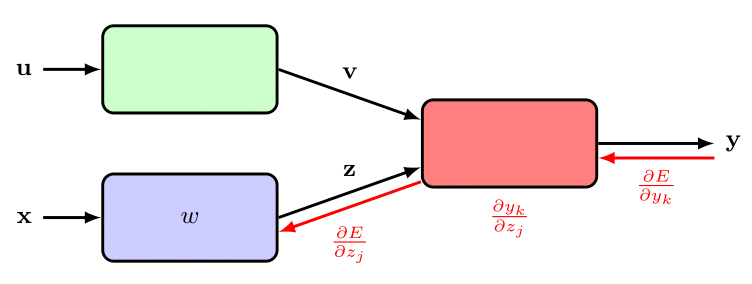
\includegraphics[width=1.0\linewidth]{Plantilla_TFG_latex/imagenes/Mat/Definicion/bp_2.png}
    \caption[Proceso de \textit{backpropagation} en una arquitectura modular de aprendizaje profundo]{Proceso de \textit{backpropagation}, donde una arquitectura modular de aprendizaje profundo en la que la matriz jacobiana se emplea para propagar hacia atrás las señales de error desde las salidas hasta los módulos anteriores en el sistema. En la imagen, las entradas $\mathbf{u}$ y $\mathbf{x}$ se procesan en módulos distintos. El módulo superior recibe $\mathbf{u}$ y produce una salida intermedia $\mathbf{v}$, mientras que el módulo inferior recibe $\mathbf{x}$, con un conjunto de pesos representados por $w$, y genera una salida intermedia $\mathbf{z}$. Ambos valores, $\mathbf{v}$ y $\mathbf{z}$, sirven como entrada para un tercer módulo (en rojo), que produce la salida final $\mathbf{y}$. Durante la propagación hacia atrás del error (indicada por las flechas rojas), la derivada del error con respecto a la salida, $\frac{\partial E}{\partial y_k}$, se propaga hacia atrás a través de la derivada $\frac{\partial y_k}{\partial z_j}$ hasta obtener $\frac{\partial E}{\partial z_j}$. Posteriormente, este error se retropropaga aún más hasta el módulo anterior, permitiendo la actualización de los pesos $w$. Imagen obtenida de \cite{bishop2023learning}.}
    \label{fig:bp_2}
\end{figure}


\subsubsection{Capa no-lineal}



Consideramos primero una capa que aplica una función no lineal, normalmente el caso de las funciones de activación. $z=\sigma(x)$, con $z^{(i)} = \sigma(x^{(i)})$. El elemento en la posición $(i,j)$ del jacobiano es dado por:

$$ \frac{\partial z^{(i)}}{\partial x^{(j)}} =  \left\{\begin{matrix}

\sigma'(x^{(i)}) \quad \textrm{si } i=j  \\
0 \quad \textrm{en otro caso.}
\end{matrix}\right .
$$

Donde $\sigma'(a) = \frac{d\sigma}{da}(a)$. En otras palabras, el jacobiano con respecto de la entrada es 

$$J=\frac{\partial \sigma}{\partial x}= diag(\sigma'(x)).$$

Si tomamos como ejemplo la función \textit{ReLU}, para un vector arbitratio $u$, podemos calcular su PVJ $u^TJ$ a través de la multiplicación  de elementos de la diagonal de $J$ con el vector $u$. 


$$\sigma(a) = ReLU(a)= max(a,0),$$
$$\sigma'(a)=
\left\{\begin{matrix}

0 \quad \textrm{si } a<0  \\
1 \quad \textrm{si } a>0.
\end{matrix}\right.
$$

Como hemos visto en la Sección \ref{sec:subgrad} la función \textit{ReLU} no es diferenciable en el punto 0, pero sí que admite subderivada en todo su dominio, y en el punto $a=0$ es cualquier valor entre $[0,1]$, y usualmente en la práctica se toma el valor 0. Por tanto

$$ReLU'(a)= \left\{\begin{matrix}

0 \quad \textrm{si } a\leq0  \\
1 \quad \textrm{si } a>0 \textrm{.} \\
\end{matrix} \right.$$

$$J=\frac{\partial \sigma}{\partial x}= diag(ReLU'(x)).$$


\subsubsection{Capa de entropía cruzada}

Consideramos ahora la capa cuya función es la función de coste, en concreto con una medición del error usando CE donde tenemos $C$ clases, que toma las predicciones $x$ y las etiquetas $y$ como entrada y devuelve un escalar. Recordamos que en esta capa la matriz jacobiana es un vector fila, identificado con el gradiente, ya que la salida es un escalar.

\begin{align*}
	z&=f(x)=CE(x,y) \\
	&= - \sum_c y_c log(softmax(x)_c) = - \sum_c y_c log(p_c)\\
\end{align*}

donde $p_c=softmax(x)_c= \frac{e^{x_c}}{\sum_{c'=1}^C e^{x_{c'}}}$ son las probabilidades de las clases predichas, e $y$ es la etiqueta correcta con codificación \textit{one-hot encoded vector}, es decir un vector de C elementos que representa la clase real a la que pertenece; si ese elemento pertenece a la clase $k$, todos las posiciones del vector $y$ serán 0 a excepción de la posición $k$, que será 1. El jacobiano con respecto a la entrada es

$$J= \frac{\partial z}{\partial x}= (p-y)^T \in \mathbb{R}^{1\times C}.$$

Vamos a asumir que la clase objetivo es la etiqueta c:

$$z=f(x)=-log(p_c)=-log \left (\frac{e^{x_c}}{\sum_j e^{x_j}} \right ) = log \left ( \sum_j e^{x_j} \right ) - x_c.$$

Entonces

$$\frac{\partial z}{\partial x_i} = \frac{\partial}{\partial x_i} log \sum_j e^{x_j} - \frac{\partial}{\partial x_i}x_c = \frac{e^{x_i}}{\sum_j e^{x_j}} - \frac{\partial}{\partial x_i}x_c = p_i - \mathbb{I}(i=c).$$

\subsubsection{Capa lineal}

Consideramos por último una capa lineal $z=f(x,W)=Wx$, donde $W \in \mathbb{R}^{m \times n}$, con $x \in \mathbb{R}^n$ y $z \in \mathbb{R}^m$ son respectivamente la entrada y la salida de esa capa.

Conviene aclarar, para evitar confusiones, que en la descripción previa hemos considerado las capas ocultas como una combinación de las operaciones lineales que aquí se describen con las funciones de activación, aquí sin embargo las analizamos por separado con el objetivo de una descripción más sencilla y un análisis más individualizado. Esta agrupación es una abstracción y por tanto no varía en cuanto a resultados.


Como $z$ es lineal, el jacobiano de la función de la capa con respecto al vector de entrada de esa capa coincide con su matriz de coeficientes, $\frac{\partial z}{\partial x}=W$

%$$z_i = \sum_{l=1}^n W_{il}x_l.$$

%El elemento que ocupa la posición $(i,j)$ en la matriz jacobiana será 

%$$\frac{\partial z_i}{\partial x_j} = \frac{\partial}{\partial x_j} \sum_{l=1}^n W_{il} x_l = \sum_{l=1}^n W_{il} \frac{\partial}{\partial x_j} x_l = W_{ij}$$

%ya que $\frac{\partial}{\partial x_j} x_l= \mathbb{I} (l=j)$. Por tanto el jacobiano con respecto a la entrada será

%$$J=\frac{\partial z}{\partial x}=W.$$

El PVJ entre $u^T \in \mathbb{R}^{1 \times m}$ y $J \in \mathbb{R}^{m \times n}$ es

$$u^T \frac{\partial z}{\partial x} = u^T W \in \mathbb{R}^{1 \times n}.$$

Ahora consideramos el jacobiano con respecto a la matriz de los pesos, $J=\frac{\partial z}{\partial W}$. Esto se puede representar como una matriz de tamaño $m \times (m \times n)$, que resulta compleja de manejar. Por tanto en lugar de eso veremos de manera individual cómo calcular el gradiente con respecto a un único peso $W_{ij}$. Esto es más sencillo de calcular ya que $\frac{\partial z}{\partial W_{ij}}$ es un vector. Para su cómputo nos fijamos en que 

$$z_l = \sum_{t=1}^n W_{lt}x_t, \qquad \textrm{y}$$

$$\frac{\partial z_l}{\partial W_{ij}} = \sum_{t=1}^n x_t \frac{\partial}{\partial W_{ij}} W_{lt} = \sum_{t=1}^n x_t \mathbb{I}(i=l \textrm{ y } j=t) .$$

Por tanto

$$\frac{\partial z}{\partial W_{ij}} = \left ( 0, \ldots, 0, x_j,  0, \ldots, 0 \right )^T$$

Donde el elemento no nulo ocupa la posición $i$-ésima. El PVJ entre $u^T \in \mathbb{R}^{1 \times m}$ y $\frac{\partial z}{\partial W} \in \mathbb{R}^{m \times ( m \times n)}$ se puede representar como una matriz de tamaño $1 \times (m \times n)$. Vemos que 

$$u^T \frac{\partial z}{\partial W_{ij}}= \sum_{l=1}^m u_l \frac{\partial z_l}{\partial W_{ij}} = u_i x_j.$$

Con lo cual

$$ u^T \frac{\partial z}{\partial W}  = ux^T \in \mathbb{R}^{m \times n}.$$



\subsubsection{Grafos computacionales}

Los MLP son un tipo de Redes Neuronales Profundas donde cada capa se conecta directamente con la siguiente formando una estructura de cadena. Sin embargo,\textbf{ las Redes Neuronales Profundas más recientes combinan componentes diferenciables de forma mucho más compleja, creando un grafo computacional de forma similar a como en la programación se combinan funciones simples para hacer otras más complejas}. La restricción es que el grafo resultante debe de ser un grafo acíclico dirigido, donde cada nodo es una función subdiferenciable. Un grafo acíclico dirigido es un tipo de grafo donde cada arista que une dos nodos tiene un sentido específico desde un nodo al otro (dirigido) y en el que no se forman ciclos, es decir, partiendo de un nodo dado no existe una secuencia de aristas dirigidas por la que se pueda volver a él.



Vamos a ver un ejemplo usando la función $f(x_1,x_2)=x_2e^{x_1}\sqrt{x_1+x_2e^{x_1}}$, cuyo grafo se puede ver representado en la Figura \ref{fig:def.grafo}.


\begin{figure}
    \centering
    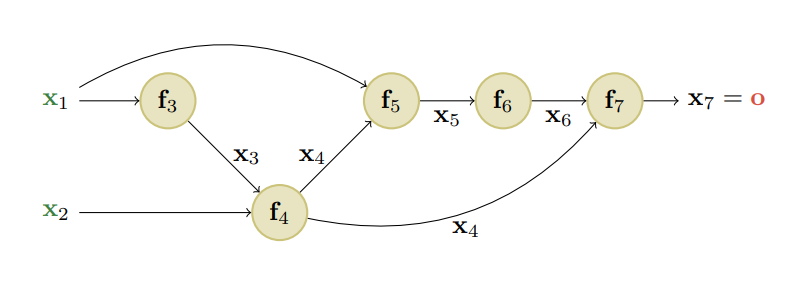
\includegraphics[width=1.0\linewidth]{Plantilla_TFG_latex/imagenes/Mat/Definicion/graf.png}
    \caption[Representación de una red computacional como un grafo dirigido acíclico para diferenciación automática y \textit{backpropagation}]{Representación de una red computacional como un grafo dirigido acíclico para diferenciación automática y BP. La figura muestra un grafo dirigido acíclico donde los nodos representan operaciones matemáticas $f_i$  y las aristas indican el flujo de información entre variables intermedias $x_i$. Las entradas $x_1$ y $x_2$ alimentan las funciones $f_3$ y $f_4$, generando las variables $x_3$ y $x_4$, que a su vez son utilizadas en pasos posteriores. El proceso continúa hasta obtener la salida final $x_7$. Esta estructura permite calcular eficientemente derivadas mediante diferenciación automática en modo de diferenciación hacia atrás, utilizada en el algoritmo de BP para optimizar redes neuronales profundas. Imagen obtenida de \cite{pml1Book}.}
    \label{fig:def.grafo}
\end{figure}


Las funciones intermedias que vemos en el grafo son:

\begin{align*}
x_3= &f_3(x_1)=e^{x_1} \\
x_4 = &f_4(x_2,x_3)=x_2x_3 \\
x_5=&f_5(x_1,x_4)=x_1 + x_4 \\
x_6=&f_6(x_5) = \sqrt{x_5} \\
x_7=&f_7(x_4,x_6)=x_4x_6 .
\end{align*}

Ahora no tenemos una estructura de cadena y en algunos casos necesitaremos sumar los gradientes a través de diferentes caminos, como es el caso del nodo $x_4$ que influye en $x_5$ y $x_7$. Para asegurar un funcionamiento correcto basta con nombrar los nodos en orden topológico (los padres antes que los hijos) y luego hacer la computación en orden topológico inverso. En general usamos

$$ \frac{\partial o }{ \partial x_j } = \sum_{k \in Hijos(j)} \frac{\partial o}{ \partial x_k} \frac{\partial x_k}{\partial x_j}.$$

En nuestro ejemplo para el nodo $x_4$:

$$   \frac{\partial o }{ \partial x_4 }  =  \frac{\partial o}{ \partial x_5} \frac{\partial x_5}{\partial x_4} +\frac{\partial o}{ \partial x_7} \frac{\partial x_7}{\partial x_4} .$$


En la práctica el grafo computacional se puede calcular previamente, usando una librería que nos permita definir un grafo estático. Alternativamente podemos calcular el grafo en tiempo real, siguiendo la ejecución de la función en un elemento de entrada. Esta segunda opción hace más fácil trabajar con grafos dinámicos cuya forma puede cambiar dependiendo de los valores calculados por la función. Por ejemplo, Tensorflow 1 usaba los grafos estáticos mientras que su versión más reciente TensorFlow 2 y PyTorch usan los grafos en tiempo real. 




\subsection{Problemas con el cálculo del gradiente}

\subsubsection{Desvanecimiento y explosión del gradiente}\label{sec:desvyexpl}


Siguiendo el hilo de la Sección \ref{sec:convergencia}, vamos a ver dos problemas que surgen a la hora de entrenar modelos usando gradiente descendente y que pueden impedir la convergencia, pero con la diferencia de que estas limitaciones en la convergencia están ligadas únicamente al algoritmo de BP, es decir, a cómo se calcula el gradiente y no a cómo se usa en la búsqueda de soluciones.

Cuando entrenamos modelos muy profundos (con muchas capas ocultas), los gradientes tienen tendencia bien a volverse muy pequeños (desvanecimiento del gradiente) o bien a volverse muy grandes (explosión del gradiente) ya que la señal de error es pasada a través de una serie de capas que o lo amplifican o lo mitigan. Esto provoca que o bien se deje de actualizar el peso del cual se desvanece su gradiente o que el gradiente diverja en el otro caso \cite{VanishExplode}. Para ver el problema con detalle, consideramos el gradiente de la función de pérdida con respecto a un nodo en la capa $l$:

$$\frac{\partial \mathcal{L}}{\partial z_l} = \frac{\partial \mathcal{L}}{\partial z_{l+1}} \frac{\partial z_{l+1}}{\partial z_l} = g_{l+1} J_l$$

donde $J_l = \frac{\partial z_{l+1}}{\partial z_l}$ es la matriz jacobiana, y $g_{l+1} = \frac{\partial \mathcal{L}}{\partial z_{l+1}}$ es el gradiente de la siguiente capa. Si $J_l$ es constante entre capas, es claro que la contribución del gradiente de la capa final $g_L$ a la capa $l$ será $ g_L J^{L-l}$. Entonces el comportamiento del sistema dependerá de los valores propios de $J$. %TODO: Referencia o explicacion??

$J$ es una matriz de valores reales pero generalmente no es simétrica, por lo que sus autovalores y autovectores pueden ser complejos, representando un comportamiento oscilatorio. Sea $\lambda$ el radio espectral de $J$, que es el máximo del valor absoluto de sus autovalores. \textbf{Si es mayor que 1, el gradiente puede explotar; y si es menor que 1 su gradiente se puede desvanecer. }

El problema de la explosión del gradiente se puede resolver de manera rápida y cómoda a través de acotar el gradiente con su magnitud y una constante $c \in \mathbb{R}^+$ en caso de que se vuelva muy grande

$$g' = min(1, \frac{c}{\|g\|}g)$$

De esta manera la norma de $g'$ nunca puede ser mayor que $c$, pero el vector apunta siempre en la misma dirección que el gradiente.

También existen otras soluciones que además son aplicables al problema del desvanecimiento de gradiente, que no se soluciona de manera tan sencilla:

\begin{itemize}
    \item Adaptar las funciones de activación para prevenir que el gradiente se vuelva muy grande o muy pequeño.

    \item Modificar la arquitectura del modelo para estandarizar las funciones de activación en cada capa, para que la distribución de las activaciones sobre el conjunto de datos permanezca constante durante el entrenamiento.

    \item Elegir cuidadosamente los valores iniciales de los pesos del modelo.
   
\end{itemize}

En la siguiente sección veremos detenidamente el último punto, ya que es la práctica más estandarizada. Existen además familias concretas de modelo que mitigan específicamente estos efectos con su arquitectura como son las ResNets, de las cuales hablaremos en la parte Informática de la memoria.


\subsubsection{Inicialización de los pesos}\label{sec:inipesos}

\textbf{Cómo inicializamos los pesos es una decisión importante a la hora de determinar cómo converge (y si lo hace) un modelo}. La convergencia o no, su velocidad y la solución a la que se converge en el entrenamiento de un modelo mediante el algoritmo de gradiente descendente es muy sensible al punto inicial desde el que comenzamos la búsqueda de una solución. Hay que remarcar que esto sucede cuando la función de error no es convexa, pero como es el caso mayoritario, lo asumimos de manera general.  

Basándonos en \cite{stabilityProblem2}, donde se observa que inicializar parámetros de una distribución normal con varianza fija puede resultar en el problema de la explosión de gradiente, vamos a ver por qué ocurre esto y, a través de añadir restricciones para evitarlo vamos a llegar a las heurísticas de inicialización de pesos más comunes.

Consideramos el pase hacia delante en una neurona lineal sin capa de activación dada por $o_i = \sum_{j=1}^{n_{in}} w_{ij}x_j$ . Suponemos $w_{ij} \sim \mathcal{N}(0, \sigma^2)$, con $\mathbb{E}[x_j]=0$ y $\mathbb{V}[x_j]=\gamma^2$, donde asumimos $x_j$ independiente de $w_{ij}$, y $n_{in}$ es el número de conexiones de entrada que recibe la neurona. La media y la varianza de la salida vienen dadas por

$$\mathbb{E}[o_i]= \sum_{j=1}^{n_{in}} \mathbb{E}[w_{ij} x_j] = \sum_{j=1}^{n_{in}} \mathbb{E}[w_{ij}] \mathbb{E}[x_j]=0$$

$$\mathbb{V}[o_i] = \mathbb{E}[o_i^2] - (\mathbb{E}[o_i])^2 = \sum_{j=1}^{n_{in}} \mathbb{E}[w_{ij}^2x_j^2] - 0 = \sum_{j=1}^{n_{in}} \mathbb{E}[w_{ij}^2] \mathbb{E}[x_j^2] = n_{in} \sigma^2 \gamma^2.$$

Para evitar que la varianza diverja, necesitamos que $n_{in} \sigma^2$ se mantenga constante. Si consideramos el pase hacia atrás y realizamos un razonamiento análogo vemos que la varianza del gradiente puede explotar a menos que $n_{out} \sigma^2$ sea constante, donde $n_{out}$ son las conexiones de salida de la neurona. Para cumplir con esos dos requisitos, imponemos $\frac{1}{2}(n_{in}+n_{out}) \sigma^2 = 1$, o equivalentemente

$$\sigma^2= \frac{2}{n_{in}+n_{out}}.$$

Esta se conoce como inicialización de Xavier o inicialización de Glorot \cite{stabilityProblem2}. Si usamos $\sigma^2= \frac{1}{n_{in}}$ tenemos un caso especial conocida como la inicialización de LeCun, propuesta por Yann LeCun en 1990. Es equivalente a la inicialización de Glorot cuando $n_{in}=n_{out}$. Si usamos $\sigma^2 = \frac{2}{n_{in}}$, tenemos la llamada inicialización de He, propuesta por Kaiming He en \cite{heinic}.


Cabe resaltar que no ha sido necesario usar una distribución Gaussiana. De hecho, las derivaciones de arriba funcionan en términos de la media y la varianza, y no hemos hecho suposiciones sobre si era Gaussiana. 


\textbf{Aunque hemos supuesto que se trataba de una neurona lineal sin función de activación que añada una componente no lineal, se conoce de manera empírica que estas técnicas son extensibles a unidades no lineales}. \textbf{La inicialización que elijamos dependerá mayoritariamente de la función de activación que usemos}. Se conoce que para funciones de activación \textit{ReLU} funciona mejor la inicialización de He, para las funciones \textit{SELU} se recomienda la inicialización de LeCun y para las funciones lineales, logística, tangente hiperbólica y \textit{Softmax} se recomienda el uso de la inicialización de Glorot \cite{pml1Book}.
\section{Conclusiones y trabajos futuros}

Al comienzo de esta parte matemática, se establecieron dos objetivos principales:

\begin{itemize}
	\item Analizar la convergencia del gradiente descendente.
	
	\item Explorar el uso de BP para este algoritmo de aprendizaje.
\end{itemize}

En primer lugar hemos introducido los conceptos y términos necesarios con los que íbamos a trabajar, y presentamos la idea original de Cauchy de la que surge el algoritmo de aprendizaje que conocemos hoy día. Luego, diferenciamos tres versiones distintas del algoritmo según la cantidad de datos que se usen para calcular el gradiente y vimos los componentes básicos de este método. También introdujimos el concepto de subgradiente, que nos permite analizar de manera rigurosa el algoritmo de gradiente descendente sin necesidad de que todas las funciones que intervienen en el modelo sean diferenciables. \textbf{Hemos visto el enunciado y demostración de un teorema que nos asegura la convergencia al mínimo global del algoritmo en su versión BGD}, aunque con condiciones muy estrictas como que la función de coste sea convexa o de clase $C^2$.

\textbf{Presentamos el concepto de martingala, un tipo de proceso estocástico con el que podemos modelar las versiones estocásticas del algoritmo de gradiente descendente}. A través del \textbf{teorema de Siegmund-Robbins}, que proporciona convergencia para las casi supermartingalas, \textbf{conseguimos demostrar un teorema que nos asegura la convergencia de SGD y MBSGD hacia un minimizador global con probabilidad 1}, consiguiendo un teorema mucho más práctico que el anterior. Aunque es necesario para ello la hipótesis, demasiado estricta, de que la función sea globalmente fuertemente convexa, \textbf{se espera que haya convergencia hacia un minimizador local en caso de que la función de coste sea fuertemente convexa a nivel local}.

\textbf{Para analizar y comprender el algoritmo de BP, hemos visto qué es la diferenciación automática y qué estrategia utiliza para realizar cálculos de manera eficiente}. Usando como ejemplo un MLP, pudimos ver cómo funciona esta técnica y distinguimos entre diferenciación hacia delante y hacia detrás. Una vez presentados estos conceptos, \textbf{exploramos propiamente el algoritmo de BP, en qué se basa y por qué resulta eficiente dicho algoritmo}. Concluimos finalmente poniendo varios ejemplos prácticos de cálculos realizados con esta técnica y resaltando problemas que trae consigo.

%Afirmamos entonces que se han cumplido los objetivos que nos habíamos planteado, no siendo una tarea sencilla. Para cumplirla ha sido necesario recordar muchos conceptos explicados durante el grado, extender algunos ya conocidos y descubrir otros completamente nuevos. Muchos conceptos sobre diferenciabilidad y probabilidad tuve que recordarlos y repasarlos minuciosamente, ya que son la base para el desarrollo posterior del trabajo.

Esto ha permitido conocer los procesos estocásticos de tipo martingala, que no solo son una herramienta poderosa para el análisis del gradiente descendente, sino que resultan una estrategia ampliamente usada para derivar resultados sobre convergencia o probar límites probabilísticos. De esta manera se buscan modelar ciertos procesos con estos objetos para aprovechar sus cualidades y propiedades.

Los conceptos de subgradiente y subdiferenciabilidad, aunque menos ampliamente usados que el anterior, constituyen un recurso indispensable en el campo del aprendizaje profundo para el análisis de técnicas relacionadas con el gradiente descendente a nivel teórico. Gracias a este trabajo he adquirido una visión más teórica y formal del aprendizaje profundo y de cómo se lleva a cabo su entrenamiento. \textbf{En un campo donde en muchas ocasiones prima el ensayo y error, adquirir una perspectiva teórica formal resulta indispensable a la hora de investigar y poder ofrecer mejoras}.

Como conclusión, creo que este trabajo me ha servido para poner en común el aprendizaje de ambos grados y gracias a él he adquirido además destreza y soltura para buscar, consultar y leer publicaciones matemáticas en este ámbito, lo cual es una habilidad muy importante.




Después de comentar los resultados obtenidos, en el futuro podrían resultar interesantes los siguientes trabajos:

\begin{enumerate}
	\item Para el Teorema \ref{teor:convsgd}, sobre la convergencia de SGD, demostrar de manera rigurosa las suposiciones que se plantean ante la relajación de las condiciones de convexidad: cuando la función de coste no es globalmente fuertemente convexa, sino que es fuertemente convexa a nivel local, entonces el algoritmo converge a un minimizador local en lugar de a uno global.
	
	\item Los procesos estocásticos de tipo martingala han demostrado ser herramientas poderosas para el análisis teórico de la convergencia de SGD. Se podrían reformular optimizadores modernos basados en GD, como Adam o RMSProp, en términos de procesos de martingalas para analizar de manera particular y más rigurosa sus propiedades de convergencia y estabilidad.
	
	%\item Se propone un análisis teórico de cómo las estrategias de inicialización de pesos afectan la propagación de la varianza y el gradiente en redes neuronales en función de la activación utilizada. Se estudiarán condiciones para evitar la saturación de activaciones y la desaparición/explosión del gradiente. Finalmente, se evaluarán estrategias existentes y se explorarán posibles mejoras en la inicialización.
\end{enumerate}



\newpage

\part{Parte informática: Estudio empírico comparativo entre gradiente descendiente y metaheurísticas para el entrenamiento de redes neuronales.}

\vspace{4cm}

\newpage



\input{Plantilla_TFG_latex/Informatica/Introducción}
\section{Fundamentos teóricos}
En esta sección se detallan los conceptos, familias de modelos y algoritmos necesarios para la elaboración del trabajo posterior. Se usarán los conocimientos aprendidos en las asignaturas de Aprendizaje Automático, Visión por Computador y Metaheurísticas además de las referencias indicadas en cada caso.


En la Sección \ref{sec:gd} aparecen los optimizadores basados en GD que se utilizarán en la experimentación: Adam, AdamW, NAG y RMSProp, mientras que en la Sección \ref{sec:mh} se hace lo propio con los algoritmos MH: SHADE y SHADE-ILS. Para finalizar, en la Sección \ref{sec:tests} se describen los tests estadísticos que más tarde se emplearán en la experimentación para un análisis riguroso de los rendimientos de los modelos.

\subsection{Redes neuronales y aprendizaje profundo}
\label{sec:profundo}

\subsubsection{Red neuronal}

Una red neuronal es un modelo computacional inspirado en la manera en la que las neuronas se conectan en el cerebro humano procesando la información. Consiste en capas interconectadas con nodos llamados neuronas, donde cada conexión tiene un peso asociado. Cada neurona normalmente aplica una función no linear, llamada función de activación, a la suma ponderada de las entradas de la capa anterior, permitiendo al modelo aprender relaciones complejas \cite{stanford_231}. Este tipo de redes se denominan totalmente conectadas. Sus componentes básicos son:

\begin{itemize}
	\item Capa de entrada: recibe la información.
	
	\item Capas ocultas: son las capas intermedias, que realizan los cálculos.
	
	\item Capa de salida: produce la salida del modelo.
\end{itemize}

El ejemplo más sencillo es el Perceptrón \cite{perceptron}, una red neuronal de una sola capa oculta y una sola neurona como podemos ver en la Figura \ref{fig:Perceptron}. Es un clasificador lineal, es decir, sólo puede resolver tareas cuyos datos sean linealmente separables. En su versión original su función de activación $f$ es la función signo. Para problemas más complejos que no sean lineales necesitamos usar redes neuronales con varias capas ocultas.


\begin{figure}
    \centering
    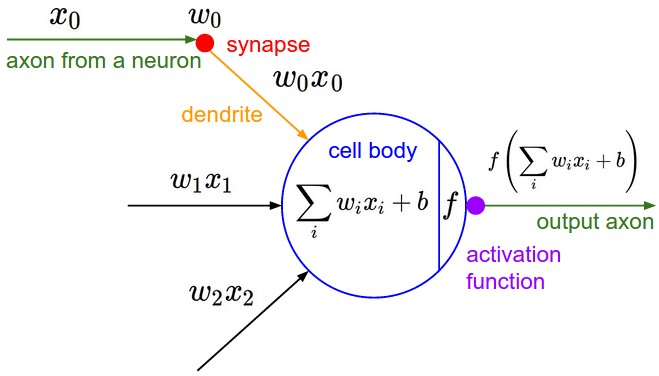
\includegraphics[width=0.75\linewidth]{Plantilla_TFG_latex//imagenes//Inf//2.Fund/neuron_model.jpeg}
    \caption[Representación esquemática de una neurona artificial inspirada en el modelo biológico]{Representación esquemática de una neurona artificial inspirada en el modelo biológico. La imagen ilustra la analogía entre una neurona biológica y una neurona artificial en una red neuronal. Las entradas $x_0,x_1,x_2$  representan señales provenientes de otras neuronas, con pesos sinápticos $w_0, w_1, w_2$ que modulan su importancia. En la biología, estas señales viajan a través del axón de una neurona y se transmiten mediante sinapsis (en rojo) a la dendrita (en naranja) de otra neurona. En la neurona artificial, las entradas ponderadas se combinan el cuerpo celular (en azul) mediante una suma ponderada $\sum_i w_ix_i + b$, donde $b$ es un sesgo. Esta combinación es procesada por una función de activación $f$ (en morado), cuya salida viaja a través del axón de salida (en verde), propagando la información a la siguiente capa de la red. Obtenida de \cite{stanford_231}.}
    \label{fig:Perceptron}
\end{figure}


\subsubsection{Aprendizaje profundo y redes neuronales profundas}

Las redes neuronales profundas tienen varias capas ocultas, generalmente más de dos. La profundidad de una red viene determinada por el número de capas ocultas que tiene, y ésta permite aprender representaciones jerárquicas de los datos, lo que habilita a las redes neuronales profundas a capturar patrones más complejos en los datos en comparación con redes con menos profundidad \cite{stanford_231}.

El aprendizaje profundo es una rama del aprendizaje automático que se centra en las redes neuronales profundas. Generalmente se usan modelos muy profundos con un alto número de parámetros y grandes cantidades de datos para resolver tareas complejas. Esto supone que se requiere de mucho poder computacional y de algoritmos avanzados para optimizar sus parámetros. Este tipo de modelos obtiene un gran rendimiento en tareas como el procesamiento del lenguaje natural, reconocimiento de voz o visión por computador. Los perceptrones multicapa son el ejemplo más clásico.





\subsubsection{Perceptrones Multicapa}

La familia de modelos que usaremos en la experimentación para las tareas de regresión será la de los Perceptrones Multicapa o \textit{Multilayer Perceptrons} (MLP), que son una versión más compleja del Perceptrón, que cuenta con varias capas ocultas y varias neuronas en cada una como el ejemplo de la Figura \ref{fig:NeuralNet}. Son capaces de procesar datos no linealmente separables ya que pueden aprender información más compleja. Sus capas son totalmente conectadas y la información fluye sólo hacia delante a la hora de hacer una predicción con el modelo \cite{GoodFellowBook}. 

En su definición original, usan la función signo como función de activación en todas las neuronas y sólo se usan para tareas de clasificación. Sin embargo actualmente son sinónimo de redes profundas totalmente conectadas, siendo usadas con cualquier tipo de función de activación y para tareas de clasificación o regresión.

\begin{figure}
    \centering
    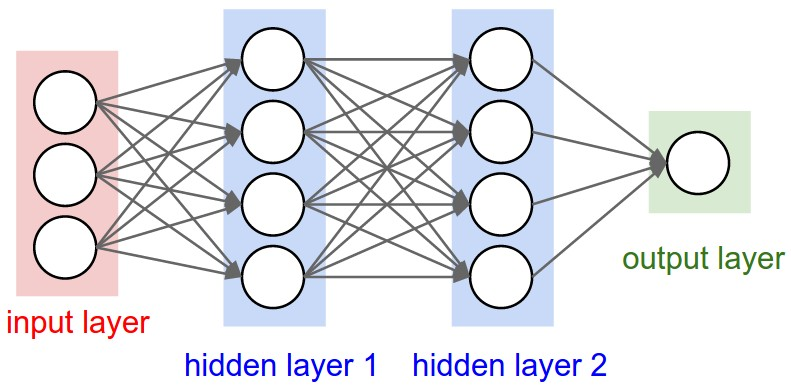
\includegraphics[width=0.75\linewidth]{Plantilla_TFG_latex//imagenes//Inf//2.Fund/neural_net2.jpeg}
    \caption[Estructura de una red neuronal profunda con dos capas ocultas]{Estructura de una red neuronal profunda con dos capas ocultas. La imagen representa una red neuronal artificial multicapa compuesta por una capa de entrada (\textit{input layer}, en rojo), dos capas ocultas (\textit{hidden layers}, en azul) y una capa de salida (\textit{output layer}, en verde). Cada neurona en una capa está completamente conectada con las neuronas de la siguiente capa mediante pesos sinápticos, representados por líneas. La capa de entrada recibe los datos del problema, las capas ocultas permiten la extracción de características y la modelización de relaciones complejas, y la capa de salida genera la predicción final. Esta arquitectura es típica en aprendizaje profundo y se entrena mediante algoritmos de optimización como el descenso de gradiente. Obtenida de \cite{stanford_231}.}
    \label{fig:NeuralNet}
\end{figure}


\subsection{Redes convolucionales}
\label{sec:convnets}

Las ConvNets o redes convolucionales son una familia de modelos de aprendizaje profundo usadas en la visión por computador. Obtienen un rendimiento al nivel del estado del arte en tareas como el reconocimiento de imágenes o la detección de objetos. Se caracterizan por tener una o varias capas (al menos una) basadas en convoluciones para luego tener una o varias capas totalmente conectadas. Las primeras sirven como extractores de características que capturan propiedades espaciales de las imágenes, mientras que las segundas sirven para clasificación \cite{GoodFellowBook}.

\subsubsection{Operación de convolución}

La convolución es una operación matemática que expresa la relación entre la entrada, la salida y la respuesta del sistema a los impulsos. En el contexto del procesamiento de señales, la convolución combina dos señales para producir una tercera \cite{GoodFellowBook}. Se define matemáticamente para funciones continuas como

$$ (f \ast g)(t) = \int_{-\infty}^{\infty} f(x)g(t-x)dx.$$

Para funciones discretas se define como

$$ (f \ast g)(t) = \sum_{x=-\infty}^{\infty} f(x)g(t-x).$$

Nos referimos a $f$ como la entrada y a $g$ como el núcleo o filtro. En el aprendizaje automático la entrada suele ser un tensor de datos y el filtro un tensor de parámetros que adaptamos con el algoritmo de aprendizaje. Ambos son de dimensión finita y asumimos que su valor es 0 en todos los puntos donde no almacenamos su valor. Por tanto en la práctica podemos implementar la sumatoria infinita como una suma finita de los elementos de un vector. Si usamos una imagen bidimensional $I$ como entrada, seguramente usaremos un filtro bidimensional $K$:

$$S(i,j) = (I \ast K)(i,j) = \sum_m \sum_n I(m,n)K(i-m,j-n).$$


Las convoluciones cumplen las siguientes propiedades:

\begin{itemize}

	\item \textbf{Conmutatividad}: $f \ast g = g \ast f$.
	
	\item \textbf{Asociatividad}: $f \ast (g \ast h ) = ( f \ast g) \ast h$.
	
	\item \textbf{Distributividad}: $f \ast (g + h) = (f \ast g) + (f \ast h)$.

\end{itemize}

La propiedad conmutativa es útil a nivel matemático pero no es demasiado práctica en la implementación de una red neuronal. Por ello muchas librerías de aprendizaje automático optan por implementar la función llamada relación cruzada en lugar de la convolución, volteando el núcleo como podemos ver en la Figura \ref{fig:3.Conv}.

$$C(i,j)= (I \cdot K)(i,j) = \sum_m \sum_n I(i+m,j+n)K(m,n).$$


\begin{figure}
    \centering
    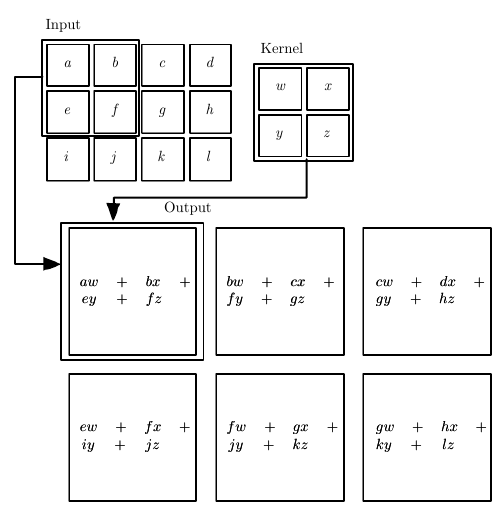
\includegraphics[width=0.5\linewidth]{Plantilla_TFG_latex//imagenes//Inf//2.Fund/Conv.png}
    \caption[Operación de correlación cruzada en una red neuronal convolucional]{Operación de correlación cruzada en una red neuronal convolucional. La imagen ilustra el proceso de correlación cruzada (\textit{cross-correlation}), una operación fundamental en redes neuronales convolucionales (ConvNets), y que es equivalente a la operación de convolución pero sin voltear el filtro. Se muestra una matriz de entrada (\textit{Input}) de 
$3 \times 4$ con elementos etiquetados ($a$ a $l$) y un kernel o filtro (\textit{Kernel}) de $2 \times 2$ con pesos ($w,x,y,z$). La operación consiste en deslizar el kernel sobre la matriz de entrada, calculando productos ponderados entre los valores superpuestos y sumando los resultados para formar la matriz de salida (\textit{Output}). Cada celda en la matriz de salida representa la suma de productos en una región local de la entrada. Este proceso permite la extracción de características espaciales en imágenes, siendo una base fundamental en la detección de patrones en ConvNets. Obtenida de \cite{GoodFellowBook}.}
    \label{fig:3.Conv}
\end{figure}


Al igual que hacen estas librerías, llamamos a estas dos operaciones indistintamente convolución, ya que en el contexto del aprendizaje de modelos no habrá diferencia, porque el algoritmo de aprendizaje obtendrá los mismos valores para el núcleo y sólo variará su posición. Podemos considerar la convolución como una multiplicación matricial donde la matriz tiene restricciones en muchas posiciones las cuales deben tener el mismo valor.

\subsubsection{Capa Convolucional}


Las capas convolucionales son las más importantes en la arquitectura de una ConvNet. Las claves de su gran rendimiento en el campo de la visión por computador son: la conectividad local, la disposición espacial y compartir parámetros \cite{GoodFellowBook}.

La conectividad local hace referencia a las conexiones de las neuronas. En entradas de alta dimensionalidad como imágenes no es práctico conectar una neurona con todas las neuronas del volumen anterior, por tanto cada neurona se conecta solo a una región local del volumen de entrada. Esto viene determinado por un hiperparámetro llamado campo receptivo, que es el tamaño del filtro que aplicamos. Mientras que las conexiones son locales en el espacio 2D (ancho y altura), siempre abarcan toda la profundidad del volumen de entrada.

Con la disposición espacial nos referimos al tamaño del volumen de salida y cómo están organizadas estas neuronas. Hay tres hiperparámetros con los que controlamos esto:

\begin{enumerate}

	\item Profundidad del volumen de salida: corresponde a la cantidad de filtros que queremos usar.
	
	\item \textit{Stride}: Indica el número de píxeles (hablando en términos de imágenes) que usamos para desplazar el filtro al realizar la convolución.
	
	\item \textit{Padding}: A veces, para mantener la dimensión de la salida es conveniente rellenar el borde de la entrada con ceros.

\end{enumerate}


Las dimensiones del volumen de salida podemos calcularlas como una función dependiente del tamaño del volumen de entrada $W$, el tamaño del filtro $F$, el \textit{stride} $S$ y el \textit{padding} $P$ que queramos aplicar. La fórmula es la siguiente:

\begin{equation}\label{eq:output}
\frac{W-F-2P}{S+1}.
\end{equation}

Esta nos dará las dimensiones en ancho y altura del volumen de salida como podemos ver en la Figura \ref{fig:stride}, y su profundidad vendrá totalmente determinada por el número de filtros que queramos usar.

\begin{figure}
    \centering
    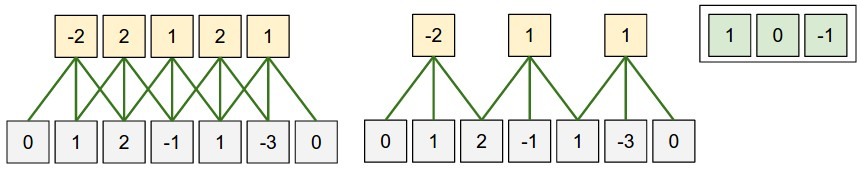
\includegraphics[width=0.75\linewidth]{Plantilla_TFG_latex//imagenes//Inf//2.Fund/2.stride.jpeg}
    \caption[Proceso de convolución en una red neuronal convolucional]{La imagen ilustra el proceso de convolución en una red neuronal convolucional. Los rectángulos grises representan las entradas, mientras que los vectores amarillos son las salidas resultantes de convolucionar las entradas con el filtro (ubicado en la esquina superior derecha). Los tamaños de las salidas pueden calcularse según la fórmula \ref{eq:output}. El filtro de tamaño $1 \times 3$ tiene valores [1, 0, -1]. El concepto de \textit{padding}, visible como bordes adicionales alrededor de las entradas, se utiliza para controlar el tamaño de las salidas. En ninguno de los dos ejemplos se usa ($P=1$). El \textit{stride}, o desplazamiento del filtro, determina cómo el filtro se mueve a través de las entradas, afectando el solapamiento y el tamaño resultante de las salidas. En el ejemplo de la izquierda se usa un \textit{stride} de $S=1$, mientras que en el de la derecha se usa $S=2$. Estos conceptos son esenciales en el aprendizaje profundo, ya que permiten ajustar la resolución y características extraídas por las ConvNets. Obtenida de \cite{stanford_231}.}
    \label{fig:stride}
\end{figure}


Compartir parámetros en una ConvNet nos permite reducir el número de éstos, reduciendo el coste del entrenamiento. Se basa en la suposición de que si una característica es útil en una posición espacial $(x,y)$ tambien lo será en otra cercana $(x',y')$. En un volumen $W \times H \times D$, en lugar de que cada neurona tenga su conjuntos de pesos, tenemos $D$ conjuntos de pesos, reduciendo drásticamente su número. 

\subsubsection{Capa \textit{Pooling}}

Su función es reducir progresivamente el tamaño de la representación para reducir el número de parámetros y la carga computacional en la red, además de controlar el sobreajuste. Opera independientemente a lo largo de la profundidad del volumen, usando la operación máximo. La opción más común es usar filtros $2 \times 2$ con un \textit{stride} $S= 2$ como se observa en la Figura \ref{fig:pooling}. La dimensión de la profundidad permanece intacta. Existen otros tipos de \textit{pooling}, por ejemplo realizar la media entre los elementos, pero esta opción fue dejando paso a la de seleccionar el máximo ya que obtiene mejores resultados en la práctica \cite{stanford_231}.

\begin{figure}
    \centering
    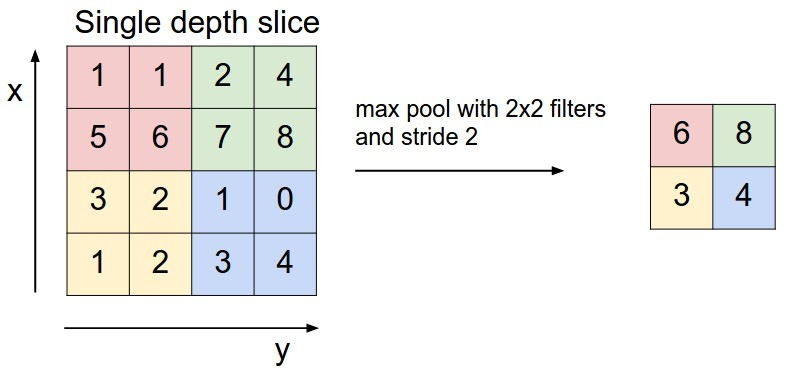
\includegraphics[width=0.75\linewidth]{Plantilla_TFG_latex//imagenes//Inf//2.Fund/maxpool.jpeg}
    \caption[Ejemplo de una operación \textit{max pooling} en una red convolucional]{La imagen muestra un ejemplo de una operación \textit{max pooling} en una ConvNet. A la izquierda, se presenta una matriz de 4x4 , con valores que van del 0 al 8. La operación de max pooling se realiza con filtros de $2\times 2$ y un \textit{stride} de 2, lo que significa que el filtro se mueve dos posiciones a la vez tanto en la dirección $x$ como en la dirección $y$. El resultado de esta operación se muestra a la derecha como una matriz de $2\times 2$, donde cada valor es el máximo de los valores en la correspondiente submatriz de $2\times 2$ de la original. Los valores resultantes son 6, 8, 3 y 4. Esta operación es relevante porque reduce la dimensionalidad de la entrada, manteniendo las características más importantes, lo que ayuda a disminuir el costo computacional y a evitar el sobreajuste en modelos de aprendizaje profundo. Obtenida de \cite{stanford_231}.}
    \label{fig:pooling}
\end{figure}

\subsubsection{Capa \textit{Batch Normalization}}

\textit{Batch Normalization} (BatchNorm) \cite{batchnorm} es un método de reparametrización adaptativa motivado por la dificultad de entrenar modelos muy profundos. En una capa de BatchNorm se estandariza la entrada a través de escalarla y trasladarla, lo que ayuda a estabilizar y acelerar el entrenamiento \cite{stanford_231}. Para cada \textit{mini-batch}, se realiza el siguiente proceso:

\begin{enumerate}

	\item Se calcula la media $\nu_{B}= \frac{1}{m} \sum_{i=1}^{m}x_i$ y la varianza $\sigma^{2}_B=\frac{1}{m} \sum_{i=1}^m(x_i - \nu_B)^2$.
	
	\item Se normaliza la entrada: $\hat{x}_i = \frac{x_i - \nu_B}{\sqrt{\sigma^{2}_B + \epsilon}}$, donde $\epsilon$ es una constante pequeña para evitar la división por 0.
	
	\item Se escala y se traslada la entrada normalizada: $y_i=\gamma \hat{x}_i + \beta$, donde $\gamma$ y $\beta$ son parámetros aprendibles por el modelo.
\end{enumerate}

Normalizando la entrada conseguimos hacer el proceso de entrenamiento más estable e intentar evitar el problema de la explosión o desvanecimiento del gradiente. También proporciona flexibilidad y mejora el rendimiento al reescalar y trasladar la entrada, y que esto dependa de parámetros aprendibles.

\subsubsection{Capa totalmente conectada}

Al final de las redes convolucionales lo más común es encontrarnos una o varias capas totalmente conectadas o \textit{fully connected} (FC), es decir, que cada neurona está conectada a todas las neuronas de la capa anterior, de la misma manera que ocurre en un MLP. Esta parte de la red permite clasificar las características extraídas por las capas convolucionales \cite{stanford_231}.

\subsection{\textit{Residual Networks}}
\label{sec:resnets}

Las \textit{Residual Networks} (ResNets) \cite{ResNets} son una familia de modelos dentro de las ConvNets que también usaremos en la experimentación, en versiones de 15 y 57 capas. Su característica principal es que usan bloques residuales, que agrupan varias capas en los cuales se suma la identidad (la entrada al bloque) a la salida del bloque. Que las redes neuronales profundas aprendan esta función identidad previene el problema de la degradación, es decir, que el rendimiento de la red decaiga a medida que aumenta el número de capas. Esto puede surgir por varias causas como la inicialización de los pesos, la función de activación o el desvanecimiento/explosión del gradiente \cite{divedeeplearning}. 

\subsubsection{Bloques residuales}

La función identidad se aprende a través de las conexiones residuales, que conectan el inicio y el final de los bloques residuales pasando la identidad. Estas conexiones además permiten aliviar el problema del desvanecimiento de gradiente. Vamos a centrarnos en una red neuronal de manera local, como se muestra en la Figura \ref{fig:resblock}. 

Si la función identidad $f(x)=x$ es el mapeo subyacente deseado, la función residual equivale a $g(x)=0$ y, por tanto, es más fácil de aprender: sólo tenemos que llevar a cero los pesos y sesgos de la última capa de pesos dentro de la línea de puntos. Con los bloques residuales, las entradas pueden propagarse más rápidamente a través de las conexiones residuales entre capas.

\begin{figure}
    \centering
    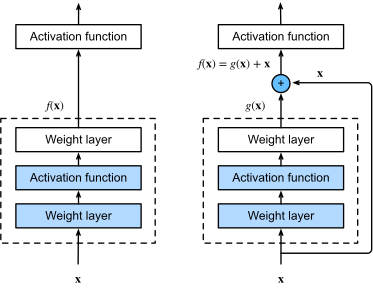
\includegraphics[width=0.75\linewidth]{Plantilla_TFG_latex//imagenes//Inf//2.Fund/resblock.png}
    \caption[Comparación entre una red neuronal tradicional y una red residual]{La imagen muestra una comparación entre una red neuronal tradicional y una red residual. En la red tradicional (izquierda), la entrada $x$ pasa a través de una capa de pesos y una función de activación para producir la salida $H(x)$. En la red residual (derecha), la entrada $x$ se suma a la salida de una capa de pesos y una función de activación, formando $H(x) + x$. Esta estructura de suma de atajos permite que la red residual aprenda funciones de identidad más fácilmente, lo que facilita el entrenamiento de redes profundas al mitigar el problema del desvanecimiento del gradiente. Obtenida de \cite{divedeeplearning}.}
    \label{fig:resblock}
\end{figure}

Para ello necesitamos que la entrada y la salida del bloque tengan el mismo tamaño. Si reducimos la dimensionalidad de la entrada o aumentamos el número de filtros entonces deberemos modificar la entrada a través de convoluciones $1 \times 1$ para que tenga el mismo tamaño que la salida, como se muestra en la Figura \ref{fig:resblock1x1}.

\begin{figure}
    \centering
    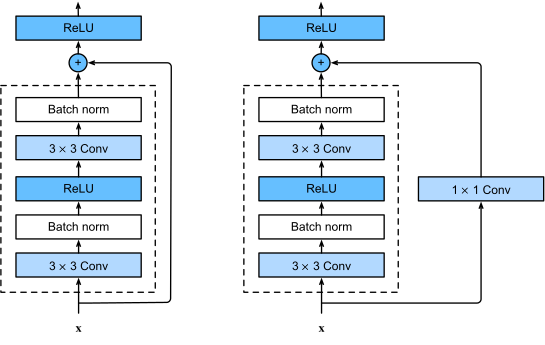
\includegraphics[width=0.75\linewidth]{Plantilla_TFG_latex//imagenes//Inf//2.Fund/resblock1x1.png}
    \caption[Bloques residuales utilizados en \textit{Residual Networks}]{La imagen muestra dos bloques residuales utilizados en ResNets. A la izquierda, se presenta un bloque residual básico que consiste en dos capas convolucionales de 3$\times$3 con una función de activación ReLU entre ellas, y una conexión de atajo que suma la entrada original al resultado de las convoluciones. A la derecha, se muestra un bloque residual con una convolución 1$\times$1 adicional, que se utiliza para ajustar las dimensiones de la entrada antes de la suma. Este bloque también incluye dos capas convolucionales de 3$\times$3 con funciones de activación ReLU entre ellas. La convolución 1x1 es crucial para permitir que la suma de la conexión de atajo sea posible cuando las dimensiones de la entrada y la salida no coinciden, mejorando así la capacidad de la red para aprender características complejas sin aumentar significativamente el costo computacional. Obtenida de \cite{divedeeplearning}.}
    \label{fig:resblock1x1}
\end{figure}

\subsubsection{Convoluciones 1x1}

%https://blog.paperspace.com/network-in-network-utility-of-1-x-1-convolution-layers/

Los bloques residuales nos permiten aumentar la profundidad de la red evitando ciertos problemas asociados, pero al añadir más capas estamos aumentando considerablemente el número de parámetros. Las convoluciones con tamaño de filtro $1 \times 1$ son una herramienta poderosa para reducir el número de parámetros manteniendo la expresividad de la red. Fueron presentadas en \cite{bottleorig}. Este tipo de convoluciones se realizan antes de realizar la convolución requerida, de manera que la dividamos en dos, una con tamaño de filtro 1 y la otra con el tamaño original.

\begin{ejemplo}
	Para ver la diferencia en el número de parámetros al usar esta herramienta, calcularemos los parámetros necesarios para realizar una convolución en el caso de tener $C=256$ canales de entrada, $O=512$ canales de salida y tamaño del filtro $F=3$.
	
	Si no usamos convoluciones $1 \times 1$, tendríamos $P= F \times F \times C \times O + O = 1.180.160$ parámetros.
	
	Usándolas debemos elegir un tamaño de filtro intermedio, por ejemplo $C'=64$. Aplicamos primero la convolución $1 \times 1$: $P'_1= 1 \times 1 \times C \times C' + C'=16.448$ parámetros. A continuación realizamos la convolución con el tamaño de filtro original: $P'_2: F \times F \times C' \times O + O=295.424$. En total, sumando las dos capas tendríamos $311.872$ parámetros, unas cuatro veces menos que en el caso anterior.
\end{ejemplo}



\subsection{Optimizadores basados en gradiente descendente}
\label{sec:gd}
Con el objetivo de intentar abordar los principales problemas del algoritmo de aprendizaje del GD se han propuesto en la literatura diversas variantes, modificando la regla de actualización de los pesos. Existen optimizadores de primer y segundo orden, en función de si hacen uso sólo de la información del gradiente o también de la matriz Hessiana, respectivamente. Vamos a ver en esta sección únicamente los de primer orden, y veremos un método de segundo orden en la sección siguiente como parte de una MH memética. Se dan tres enfoques en este ámbito: el uso de momento, tasas de aprendizaje adaptativas y la combinación de los dos anteriores. De cada uno hacemos hincapié en el que vamos a usar en el presente TFG, en orden respectivo: NAG, RMSProp, Adam y AdamW.

\subsubsection{NAG}

El algoritmo del GD es problemático en regiones de la función de error donde una dimensión tiene mucha más pendiente que otra, que son comunes alrededor de óptimos locales. En estos escenarios el algoritmo oscila y realiza poco progreso real. El momento \cite{momentumorig} es un método que acelera al algoritmo en la dirección relevante y compensa las oscilaciones, como podemos ver en la Figura \ref{fig:momentum}. Esto se realiza añadiendo una fracción $\gamma$ del vector gradiente de la última iteración al vector gradiente actual \cite{divedeeplearning, GoodFellowBook}.

\begin{figure}[!tbp]

  \centering
  \subfloat{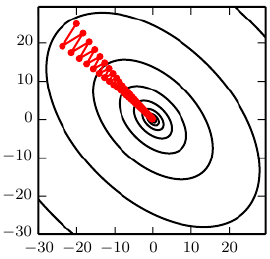
\includegraphics[width=0.4\textwidth]{Plantilla_TFG_latex//imagenes//Inf//2.Fund/sgdwoutmom.png}}
  \hfill
  \subfloat{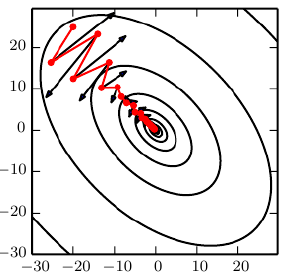
\includegraphics[width=0.4\textwidth]{Plantilla_TFG_latex//imagenes//Inf//2.Fund/sgdwmom.png}}
  \caption[Comparación entre el algoritmo de gradiente descendente estocástico original y usando el momento]{Comparación entre el algoritmo de GD estocástico original (izquierda) y usando el momento (derecha). Vemos que en la figura de la derecha se diferencia la dirección del gradiente (flechas negras) y el camino seguido por el algoritmo en rojo. Se observa que usando el momento se producen oscilaciones al principio que se van reduciendo a lo largo de la ejecución del algoritmo. Usando el momento se necesitan menos iteraciones para converger. Imágenes obtenidas de \cite{GoodFellowBook}.}
    \label{fig:momentum}
\end{figure}

\begin{align*}	
	v_t&= \gamma v_{t-1} + \eta \nabla C(W_t) \\
	W_{t+1} &= W_t- v_t. \\
\end{align*}

El valor de $\gamma$ se sitúa normalmente alrededor de 0.9. El término del momento se incrementa en las dimensiones en las que el gradiente apunta en la misma dirección y se reduce en las que el gradiente cambia de dirección, consiguiendo una convergencia más rápida y estable. Dotamos al algoritmo de cierta inercia para reducir la brusquedad en los cambios de dirección.

El optimizador \textit{Nesterov Accelerated Gradient} (NAG) \cite{Nesterov} modifica esta idea de manera que podamos ``predecir'' a dónde nos lleva esa inercia. A la hora de calcular el gradiente de la función de coste, no lo hacemos respecto a los parámetros, sino respecto a una aproximación de los parámetros tras la iteración actual, de manera que podamos saber de forma aproximada dónde nos encontraremos después de actualizar los pesos. Se puede interpretar como una corrección del método de momento original. El valor del momento se sitúa también alrededor de 0.9.

\begin{align*}	
	v_t&= \gamma v_{t-1} + \eta \nabla C(W-v_t) \\
	W_{t+1} &= W_t - v_t. \\
\end{align*}

Mientras que usando el optimizador momento original primero calculamos el gradiente y luego realizamos un salto grande en la dirección del gradiente acumulado, NAG primero realiza un salto grande en la dirección del gradiente acumulado, mide el gradiente y despúes realiza una corrección. Esta comparación se ilustra en la Figura \ref{fig:NAG}. Esta estrategia previene al algoritmo de avanzar demasiado rápido. 

\begin{figure}
    \centering
    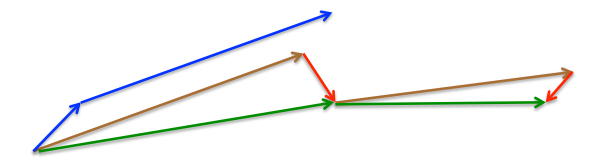
\includegraphics[width=0.75\linewidth]{Plantilla_TFG_latex//imagenes//Inf//2.Fund/NAG.png}
    \caption[Comparación del cálculo del tamaño del paso entre los métodos del momento original y el momento de Nesterov]{Comparación entre los métodos del momento original (vectores azules) y el momento de Nesterov, que muestra el paso en dos iteraciones del algoritmo de GD para mostrar las diferencias en su cálculo. En este último, primero realizamos un salto grande en la dirección del gradiente acumulado (vector marrrón) para luego medir el gradiente de la posición al acabar el salto y realizar una corrección (vector rojo). La flecha verde indica la posición final corregida donde acaba una iteración del método NAG. Obtenida de \cite{rmsprop}.}
    \label{fig:NAG}
\end{figure}


\subsubsection{RMSProp}

RMSProp (Root Mean Square Propagation) es un optimizador de primer orden que introduce tasas de aprendizaje adaptativas. Presentado por Geoff Hinton en sus materiales docentes \cite{rmsprop}, la fórmula de actualización de los pesos es la siguiente:

\begin{align*}
	E[g]_t &= 0.9 E[g]_{t-1} + 0.1 \nabla C(W_t)^{2}\\
	W_{t+1} &= W-t - \frac{\eta}{\sqrt{E[g_t^2]_t + \epsilon}}\nabla C(W_t)
\end{align*}

Donde $E[g^2]_t$ es la media móvil en la iteración $t$, que depende solamente de la iteración anterior y del gradiente actual. Las operaciones anteriores se realizan elemento a elemento, es decir, cada peso recibe una actualización con un factor personalizado. Actualizando los pesos de esta forma, cuando el gradiente es grande en una dirección entonces el factor de ese peso será pequeño, evitando oscilaciones; mientras que si en otra dirección el gradiente es relativamente pequeño entonces el valor será grande, acelerando el proceso de entrenamiento.

Existen otros optimizadores que usan tasas de aprendizaje variables como Adagrad \cite{adagrad}, sus diferencias residen en la ventana de iteraciones y el cálculo del factor de multiplicación del peso. En este optimizador sólo se tienen en cuenta la iteración pasada y la actual, mientras que el uso de una media exponencial decreciente permite que las tasas de aprendizaje no se vuelvan demasiado pequeñas \cite{divedeeplearning, GoodFellowBook}.

\subsubsection{Adam}

\textit{Adaptative Moment Estimation} (Adam) \cite{Adam} es otro método que calcula tasas de aprendizaje adaptativas para cada parámetro. Además mantiene una media exponencial decreciente de gradientes de iteraciones anteriores $m_t$ similar al momento.

\begin{align*}
	m_t&= \beta_1 m_{t-1} + (1-\beta_1)\nabla C(W) \\
	v_t&= \beta_2 v_{t-1} + (1-\beta_2)\nabla C(W)^2.
\end{align*}

$m_t$ y $v_t$ son estimaciones del momento de primer orden (media) y de segundo orden (varianza no centrada) de los gradientes, respectivamente. Son inicializados como vectores de 0, por lo que sus autores encontraron que tenían un sesgo al 0, especialmente durante las primeras iteraciones y cuando $\beta_1$ y $\beta_2$ son próximos a 1. Por tanto se calculan nuevas variables corrigiendo el sesgo:

\begin{align*}
	\hat{m}_t&=\frac{m_t}{a-\beta_1}\\
	\hat{v}_t&=\frac{v_t}{1-\beta_2}.
\end{align*}

Ahora se usan para ajustar los parámetros como hemos visto en el optimizador anterior:

$$W_{t+1} = W_t - \frac{\eta}{\sqrt{\hat{v}_t} + \epsilon} \hat{m}_t$$

Los autores proponen valores por defecto de 0.9 para $\beta_1$, 0.999 para $\beta_2$ y $10^{-8}$ para $\epsilon$ \cite{divedeeplearning, GoodFellowBook}.

\subsubsection{AdamW}

AdamW (Adam con Weight decay) \cite{AdamW} es una modificación de Adam que arregla un error de implementación, desacoplando la regularización de la actualización del gradiente. En lugar de incorporar el decaimiento de pesos en el cálculo de gradiente, como en Adam original, AdamW directamente modifica los parámetros tras el paso de actualización del gradiente añadiendo una pequeña fracción del término de decaimiento de pesos, lo que conlleva una regularización más efectiva.


$$W_t = W_{t-1} - \eta \cdot \frac{\hat{m}_t}{\sqrt{\hat{v}_t} + \epsilon} - \lambda \cdot W_{t-1}$$

\subsubsection{L-BFGS-B}\label{sec:l-bfgs}


En el presente TFG utilizamos L-BFGS-B no como optimizador a utilizar en la experimentación, sino como componente del algoritmo SHADE-ILS. Aun así, este es en sí mismo un optimizador basado en gradiente, por lo cual aparece en esta sección.

El método L-BFGS-B (\textit{Limited-memory Broyden-Fletcher-Goldfarb-Shanno with Box constraints}) \cite{L-BFGS-B} es un algoritmo Quasi-Newton, es decir, un algoritmo de optimización iterativo. Los métodos de Newton usan la matriz Hessiana de la función a optimizar para usar más información del problema y ofrecer una convergencia más rápida y estable. Para problemas complejos de  dimensionalidad elevada, calcular la Hessiana en cada paso es una tarea computacionalmente inabarcable, y los métodos de Quasi-Newton implementan una aproximación de la Hessiana para rebajar esta carga computacional. Estos métodos se diferencian entre ellos principalmente en la forma de aproximar la matriz Hessiana \cite{Numerical_optimization}.

Uno de los métodos Quasi-Newton más populares es BFGS \cite{BFGS}, que usa una aproximación de la Hessiana de forma que mantiene su propiedad de definida positiva, lo que asegura una convergencia estable. Sin embargo, aunque se reduce el coste computacional, para almacenar la matriz Hessiana se requiere demasiada memoria. El método L-BFGS \cite{L-BFGS}, en lugar de guardar una matriz con $n \times n$ aproximaciones, guarda únicamente un vector de tamaño $n$ que guarda todas las aproximaciones de manera implícita. Esta variante está diseñada para problemas de alta dimensionalidad, y produce resultados similares a su versión sin la memoria limitada \cite{stanford_231}.

La última variante L-BFGS-B, que usamos en el presente TFG en el algoritmo SHADE-ILS, es una modificación que maneja restricciones en los valores de las variables, lo que la hace incorporar información sobre el dominio. Al usar información del gradiente y de la Hessiana, es un optimizador de segundo orden, aunque es mucho menos popular que los optimizadores de primer orden. Aunque mejora la rapidez y estabilidad de la convergencia al usar más información del problema y proporciona mejores soluciones, los problemas de aprendizaje automático a día de hoy han adquirido una dimensionalidad demasiado alta para que este tipo de métodos resulten computacionalmente asequibles, y se prefiere usar los de primer orden. Aún así vemos que se implementa dentro del algoritmo de SHADE-ILS con resultados muy satisfactorios, no usándose como método de optimización principal sino de manera complementaria al algoritmo SHADE \cite{Numerical_optimization}.


\subsection{Metaheurísticas}
\label{sec:mh}

En su definición original las MH son métodos que combinan técnicas de mejora local con estrategias de alto nivel para crear un proceso capaz de escapar óptimos locales y realizar una búsqueda robusta del espacio de soluciones. Aunque no hay garantía teórica de que puedan encontrar la solución óptima, su rendimiento es muy superior en algunos casos al de algoritmos exactos que requieren demasiado tiempo para completar su ejecución, especialmente en problemas complejos del mundo real. En problemas NP-Difícil por ejemplo se prioriza el uso de MH que dan una solución cercana a la óptima en un tiempo mucho menor que algoritmos exactos \cite{mhhandbook}.

Podemos clasificar a las MH en dos grandes grupos en función de cómo se realiza la búsqueda por el espacio de soluciones: basadas en trayectorias y basadas en poblaciones. En las primeras el proceso de búsqueda se caracteriza por realizar una trayectoria en el espacio de búsqueda, que puede ser visto como la evolución en tiempo discreto de un sistema dinámico. En las MH basadas en poblaciones, en cada iteración hay un conjunto de soluciones que interactúan entre sí. Nos centraremos en este último tipo ya que es el que vamos a usar \cite{mhhandbook}.

\subsubsection{Metaheurísticas basadas en poblaciones}

Son técnicas de optimización probabilística que con frecuencia mejoran a otros métodos clásicos, e intentan imitar el mecanismo de evolución de la naturaleza a través de similitudes con la genética, como se ilustra en la Figura \ref{fig:cruce_mh}. Tiene un conjunto de soluciones denominado población, donde cada solución se llama individuo, y son generados de forma aleatoria. En cada iteración o generación, estos individuos se recombinan entre sí para intentar obtener mejores soluciones cuyo rendimiento es medido con una función objetivo. Las etapas de cada generación se pueden ver esquemáticamente en la figura \ref{fig:gen_alg}, y son:

\begin{figure}
    \centering
    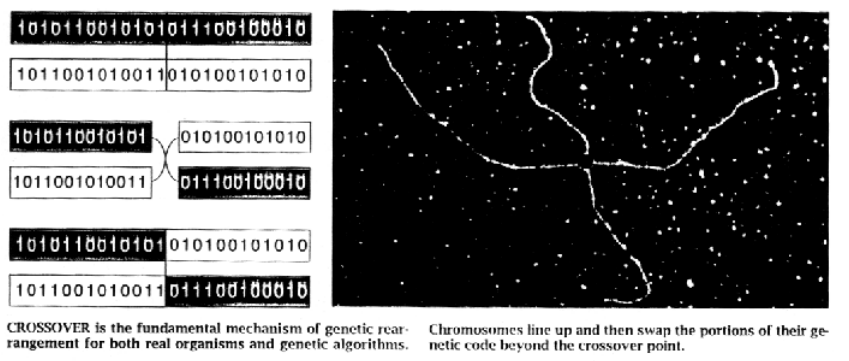
\includegraphics[width=0.75\linewidth]{Plantilla_TFG_latex//imagenes//Inf//2.Fund/cruce_mh.png}
    \caption[Representación y cruce de cromosomas en algoritmos genéticos]{La imagen ilustra la representación y el proceso de cruce de cromosomas en algoritmos genéticos. A la izquierda, se muestra un cromosoma compuesto por una cadena de bits (1 y 0) en la parte superior destacando un gen específico dentro del cromosoma. A la derecha, se presenta el proceso de cruce (corte) entre dos cromosomas parentales a través del operador de cruce en un punto. Los cromosomas parentales, representados por las cadenas '1111111' y '0000000', se cortan en un punto específico, intercambiando segmentos para formar dos nuevos cromosomas hijos: '1110000' y '0001111'. Este proceso es fundamental en los algoritmos genéticos, ya que permite la combinación y variación de información genética para la optimización y solución de problemas complejos.}%https://revistamarina.cl/es/articulo/metodos-metaheuristicos-caso-algoritmos-geneticos-en-construccion-naval
    \label{fig:cruce_mh}
\end{figure}

\begin{itemize}
	\item Selección: se elige una parte de la población actual, normalmente con criterios elitistas (se elige a los mejores) aunque introduciendo cierta aleatoriedad. Si el número de individuos elegidos es igual al tamaño de la población, hablamos de un modelo generacional, mientras que si es menor hablamos de un modelo estacionario. 
	\item Cruce: Los individuos seleccionados se agrupan por parejas y se combinan a través del operador de cruce. Las soluciones resultantes se denominan hijos. Operadores comunes son el cruce en un punto, el cruce en dos puntos y el cruce uniforme. 
	\item Mutación: A los hijos se les aplican cambios aleatorios en sus valores para mantener cierta diversidad genética en la población.
	\item Reemplazo: Se reemplaza la población actual con la nueva generación. Podemos reemplazarla entera o aplicar criterios elitistas, como reemplazar sólo con los mejores o reemplazar sólo si la nueva generación es mejor que la anterior.
	\item Terminación: se comprueba si se cumple la condición de parada. Criterios comunes son un número máximo de iteraciones o la convergencia de la población (falta de mejoras entre generaciones).
\end{itemize}

\begin{figure}
    \centering
    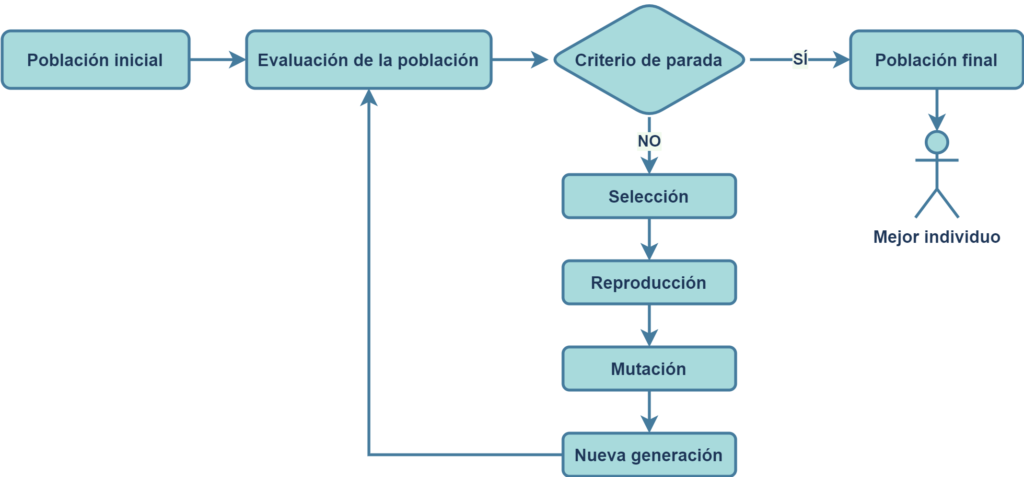
\includegraphics[width=0.75\linewidth]{Plantilla_TFG_latex//imagenes//Inf//2.Fund/alg_gen.png}
    \caption[Etapas de un algoritmo genético]{La imagen presenta un diagrama de flujo de un algoritmo genético, que incluye los siguientes pasos: iniciar con una ``Población inicial'', donde se crea una población de posibles soluciones, que se somete a una ``Evaluación de la población'', en la que cada individuo se puntúa según una función objetivo. Si se cumple el ``Criterio de parada'', se obtiene la ``Población final'' y se identifica el ``Mejor individuo''. Si el criterio no se cumple, se procede a la ``Selección'' de individuos, donde se seleccionan los individuos que se reproducirán a través de un proceso predefinido que asegure diviersidad en la población y buenas solucions, seguida de los procesos de ``Reproducción'' y ``Mutación'', en los que se cruzan los individuos seleccionados y luego se les aplica una pequeña modificación, respectivamente; para generar una ``Nueva generación''. Este ciclo se repite hasta que se cumple el criterio de parada, optimizando las soluciones tras cada generación. Obtenida de \url{https://blogs.imf-formacion.com/blog/tecnologia/}}
    \label{fig:gen_alg}
\end{figure}

Los criterios elitistas hacen que la convergencia sea más rápida, pero podemos caer en una convergencia prematura por la falta de diversidad que conllevan estos criterios, de manera que nuestro algoritmo pare antes de encontrar una solución lo suficientemente buena.



\subsubsection{\textit{Differential Evolution}}


Los algoritmos de DE \cite{diffev} son modelos basados en poblaciones que son particularmente efectivos para problemas de optimización continuos. Enfatizan la mutación y la realizan antes de aplicar el operador de cruce. Usan los parámetros factor de mutación $F$ y probabilidad de cruce $C_r$ \cite{diffevbook}. Las etapas que varían, descritas en el orden que se realizan en cada generación, son las siguientes:

\begin{itemize}
	\item{Operador de mutación: Para cada solución $x_i$ de la población, se genera un vector mutante $v_i$ a partir de la siguiente expresión:
	
	$$v_i = x_{r1} + F \cdot (x_{r2} - x_{r3}).$$
	
	Donde $x_{r1}, x_{r2}$ y $x_{r3}$ son individuos seleccionados aleatoriamente con las restricciones de que $x_i  \neq x_{rj}$ y $x_{rj} \neq x_{rj'}$ con $j, j' \in \left \{ 1,2,3 \right \}$. $F$ se suele situar en la práctica ente 0 y 2.		
	}
	
	\item{Cruce: se combinan el vector solución de partida $x_i$ y el vector mutante $v_i$ para generar el vector de prueba $u_i$. Se usa el cruce binomial:
	
	$$u_{ij} = \begin{cases}
		v_{ij} & \text{si } \text{rand}_j(0,1) \leq C_r \\
		x_{ij} & \text{en otro caso}
		\end{cases} $$
		
		donde $\text{rand}_j(0,1)$ es generado aleatoriamente con una distribución uniforme entre 0 y 1 para cada componente $j$.	
	}
	
	\item{Selección: se compara el valor de la función objetivo de los vectores iniciales con el de los vectores de prueba correspondientes, y el que tenga mayor valor pasa a la generación siguiente.}

\end{itemize}

En el pseudocódigo del Algoritmo \ref{alg:de} podemos apreciar el cambio de orden en las etapas de cada generación con respecto al esquema general de los algoritmos basados en poblaciones que veíamos en la Figura \ref{fig:gen_alg}.

\begin{algorithm}
\caption{Esquema general de DE}
\label{alg:de}
	\begin{algorithmic}
		\State $t:=0$
		\State Inicializar Pob$_t$
		\State Evaluar $x \quad \forall x \in$ Pob$_t$
		\While{No se cumpla condición de parada}
			\State $t:=t+1$			
			\State Mutar Pob$_t$ para obtener Pob'
			\State Recombinar Pob' y Pob para obtener Pob'' 
			\State Evaluar Pob''			
			\State Reemplazar Pob$_t$ a partir de Pob'' y Pob$_{t-1}$
		\EndWhile
		
		
		\Return $x_i \in Pob_t : f(x_i)\leq f(x_j)$
	\end{algorithmic}
\end{algorithm}		
		
	



\subsubsection{SHADE}

SHADE (\textit{Success-History based Adaptative Differential Evolution}) \cite{shade} es una variante avanzada del algoritmo original de DE. Consigue mejorar éste a través de guardar información histórica sobre configuraciones de los parámetros de factor de mutación ($F$) y el ratio de cruce ($CR$) que han tenido buenos resultados para poder ajustar de manera adaptativa estos parámetros y guiar el proceso de evolución, su pseudocódigo puede observarse en el Algoritmo \ref{alg:shade}. 

Los mecanismos de cruce y de selección son los mismos que en DE, variando principalmente el mecanismo de mutación. Para generar el vector mutante $v_i$ a partir de la solución $x_i$, SHADE usa la siguiente estrategia\footnote{Esta es la estrategia original, existen más modificaciones, aunque basadas en esta propuesta}:

$$v_i = x_{r1} + F \cdot (x_p - x_i)  + F \cdot (x_{r1} - x_{r2}).$$

Donde $x_p$ es un individuo seleccionado aleatoriamente de entre los $p$ mejores de la población y que es distinto a $x_i$. También se verifica que $x_i  \neq x_{rj}$ y $x_{rj} \neq x_{rj'}$ con $j, j' \in \left \{ 1,2 \right \}$. En el algoritmo de SHADE se usa $p=1$, es decir, se elige al mejor individuo de la población.

El algoritmo inicia los parámetros de factor de mutación y ratio de cruce al valor 0.5, y los va adaptando según se va ejecutando. Para ello mantiene un archivo de memoria, que se actualiza al final de cada generación y en el que se guardan parejas de los valores de los dos parámetros que han dado lugar a mejores soluciones. Al actualizar el archivo se usa la media de Lehmer\footnote{$Lehmer(X) = \frac{\sum_{x\in X} x^2}{\sum_{x\in X} x}$}  de manera que se le da más peso a las parejas de parámetros que mejor rendimiento obtienen. Al comienzo de cada generación el algoritmo obtiene valores de $F$ y $C_r$ para cada individuo basándose en el archivo de memoria e introduciendo pequeñas modificaciones.


%REVISAR PSEUDOCODIGO
\begin{algorithm}
\caption{Algoritmo SHADE}
\label{alg:shade}
	\begin{algorithmic}
		\State $t:=0$
		\State Inicializar Pob$_t$
		\State Inicializar $A$ (archivo externo)
		\State Inicializar $M$ (memoria de parámetros)
		\State Evaluar $x \quad \forall x \in$ Pob$_t$
		\While{evals $<$ total\_evals}
			\State $t:=t+1$
			\State Seleccionar $p$ soluciones para la mutación
			\State Mutar Pob$_{t-1}$ para obtener Pob'
			\State Recombinar Pob' y Pob$_{t-1}$ para obtener Pob''
			\State Evaluar Pob''
			\State Actualizar $A$ y $M$ a partir de Pob'' y Pob$_{t-1}$
			\State Obtener Pob$_t$ a partir de Pob'' y Pob$_{t-1}$
		\EndWhile
		
		
		\Return $x_i \in$ Pob$_t : f(x_i) \leq f(x_j) \quad \forall j$
	\end{algorithmic}
\end{algorithm}

SHADE está basado en DE, una familia de algoritmos de optimización que ofrece muy buenos resultados con parámetros continuos. En este ámbito, SHADE obtiene resultados del estado del arte en espacios de búsqueda de media-alta dimensionalidad, aunque no tan alta como el caso del entrenamiento de modelos de aprendizaje profundo \cite{shade}. En tareas donde la dimensionalidad es muy eleveda como la optimización de parámetros de grandes modelos, su versión memética SHADE-ILS, que veremos a continuación, consigue muy buenos resultados.



\subsubsection{Algoritmos meméticos}

Los algoritmos meméticos son técnicas de optimización MH basadas en el interacción entre componentes de búsqueda globales y locales, y tienen la explotación de conocimiento específico del problema como uno de sus principios. De manera general se componen principalmente de un algoritmo basado en poblaciones al cual se le ha integrado un componente de búsqueda local \cite{mhhandbook}.

Su principal diferencia con los algoritmos evolutivos tradicionales es que usan de manera concienzuda todo conocimiento disponible acerca del problema. Esto no es algo opcional sino que es una característica fundamental de los algoritmos meméticos. Al igual que los algoritmos genéticos se inspiran en los genes y la evolución, estas estrategias se inspiran en el concepto de ``meme'', análogo al de gen pero en el contexto de la evolución cultural. Normalmente se llama ``hibridar'' a incorporar información del problema a un algoritmo de búsqueda ya existente y que no usaba esta información.

Esta característica de incorporar información del problema está respaldada por fuertes resultados teóricos. En el teorema \textit{No Free Lunch} \cite{nofreelunch} se establece que un algoritmo de búsqueda tiene un rendimiento acorde con la cantidad y calidad de información del problema que usa. Más precisamente, el teorema establece que el rendimiento de cualquier algoritmo de búsqueda es indistinguible de media de cualquier otro cuando consideramos el conjunto de todos los problemas. 

\subsubsection{SHADE-ILS}
\label{sec:shade-ils}


SHADE-ILS \cite{shadeils} es un algoritmo memético para problemas de optimización continua a gran escala. Combina la exploración del algoritmo basado en poblaciones SHADE, usado en cada generación para evolucionar a la población de soluciones, con la explotación de una búsqueda local que se aplica a la mejor solución que se tenga en esa generación. 

En la parte de búsqueda local, en el algoritmo original existe un mecanismo de elección para usar entre varias búsquedas locales, una de ellas L-BFGS-B. En el presente TFG se ha decidido usar sólo esta última, por facilidad de implementación y porque usa más información específica del problema. Por tanto no se detallará este mecanismo de elección entre búsquedas.

Las características fundamentales de esta técnica y que la diferencia con respecto a otros algoritmos meméticos son la elección de los algoritmos empleados (tanto el de búsqueda local como el basado en poblaciones) y su mecanismo de reinicio. Éste se activa cuando a lo largo de tres generaciones el rendimiento de la mejor solución no supera en más de un 5\% al de la anterior. En dicho caso, se elige una solución aleatoria de la población y se le aplica una pequeña perturbación usando una distribución normal y el resto de la población se vuelve a generar aleatoriamente. Cuando ocurre esto los parámetros adaptativos son reiniciados a los valores por defecto.

Cabe destacar que esto se realiza ya que SHADE-ILS mantiene los parámetros adaptativos del algoritmo SHADE entre generaciones. Esto tiene mucho sentido ya que al finalizar una ejecución de dicho algoritmo, sólo aplicamos búsqueda local a una solución, con lo que la gran mayoría de la población queda intacta y por tanto podemos reutilizar estos parámetros que se han ido adaptando a ella. 

SHADE-ILS mantiene un variable para guardar la mejor solución hasta ahora y otra para guardar la mejor solución desde el último reinicio, devolviendo la primera cuando finaliza el algoritmo. En la versión utilizada se ha añadido además un array para guardar el histórico de las mejores soluciones junto con su fitness correspondiente, de manera que podamos analizar y representar las mejoras que realiza el algoritmo. 


\begin{algorithm}
\caption{Algoritmo SHADE-ILS}
\label{alg:shade-ils}
	\begin{algorithmic}
		\State $t := 0$
		\State Inicializar Pob$_t$
		\State $x_0 :=$ (maximo+minimo)/2
		\State $x_{\text{best}} := \text{L-BFGS-B}(x_0)$
		\State $x_{\text{global}} := x_{\text{best}}$
		
		\While{evals $<$ total\_evals}
			\State $t := t+1$
			\State $f_{\text{prev}} := f(x_{\text{best}})$
			\State $x_{\text{best}}, \text{Pob}_t := \text{SHADE}(\text{Pob}_{t-1})$
			\State $x_{\text{best}} := \text{L-BFGS-B}(x_{\text{best}})$
			\State $\Delta f := \frac{f_{\text{prev}} - f(x_{\text{best}})}{f_{\text{prev}}} \times 100$
			
			\If{$f(x_{\text{best}}) < f(x_{\text{global}})$}
				\State $x_{\text{global}} := x_{\text{best}}$
			\EndIf
			
			\If{$\Delta f < 5$}
				\State $g := g + 1$
			\Else
				\State $g := 0$
			\EndIf
			
			\If{$g \geq 3$}
				\State Reiniciar población conservando $x_{\text{best}}$ con perturbación normal
				\State $g := 0$
			\EndIf	
		\EndWhile
		
		\Return $x_{\text{global}}$
	\end{algorithmic}
\end{algorithm}


Vemos el pseudocódigo de la implementación realizada en el Algoritmo \ref{alg:shade-ils} y aclaramos algunas cosas que pueden no haber quedado del todo claras en favor de la claridad del pseudocódigo. Cuando generamos la población inicial, seleccionamos la peor y la mejor solución y la combinamos haciendo una media de sus elementos. A esa solución se le aplica la búsqueda local y se incluye en la población reemplazando a la peor solución. Se guardan los valores de mejora de las últimas 3 generaciones y en caso de que todas estén por debajo del 5\% se activa el mecanismo de reinicio.



En el artículo su publicación \cite{shadeils} se atienden tres cuestiones, todas a través de técnicas MH: diseño de la arquitectura, optimización de hiperparámetros y entrenamiento de los parámetros de un modelo. Nos centraremos en la última. Se utilizan seis conjuntos de datos distintos con diferente complejidad, y en base a ésta, se elige una arquitectura de modelo concreta dentro de la familia de las ConvNets, de manera que tenga buen rendimiento en su entrenamiento a través de GD. Se utiliza el optimizador Adam. En el entrenamiento con SHADE-ILS se utilizan diferentes estrategias que hacen uso de la estructura por capas de los modelos de aprendizaje profundo, realizando el entrenamiento en los pesos de diversas capas, según la estrategia, mientras se mantienen congelados los demás. También se realiza el entrenamiento de todo el modelo a la vez.

Los resultados de la experimentación son claros: solo en una de las seis tareas el modelo entrenado con SHADE-ILS minimiza más la función de pérdida que el modelo entrenado con GD. Además, en todos los casos, el error de test es mayor. Cabe mencionar que la generalización en los modelos es bastante buena, manteniéndose estos errores en valores cercanos a los que se obtiene en el entrenamiento, y aumentando el error en proporciones similares a lo que lo hace el modelo entrenado con Adam.

\subsection{Tests estadísticos}

Un test estadístico es una herramienta utilizada para evaluar hipótesis sobre una población basada en una muestra de datos. Formalmente, un test estadístico se define como un procedimiento que, dado un conjunto de datos observados, proporciona una regla de decisión para aceptar o rechazar una hipótesis nula $H_0$, en función de la evidencia contenida en los datos. La hipótesis alternativa $H_1$ representa la afirmación contraria a $H_0$.

El p-valor representa la probabilidad de obtener un resultado tan extremo como el observado, bajo la suposición de que la hipótesis nula es verdadera. En otras palabras, mide la evidencia en contra de $H_0$: valores pequeños de $p$ indican que la muestra es poco probable, lo que respalda la hipótesis alternativa $H_1$. Generalmente, se establece un umbral de significancia $\alpha$, comúnmente 0.05 o 0.01, y para p-valores por debajo de ese umbral se rechaza la hipótesis nula.

Los tests estadísticos pueden clasificarse en diferentes categorías según su propósito, como tests paramétricos y no paramétricos, tests de comparación de medias, tests de independencia y tests de ajuste a una distribución específica. Los tests paramétricos asumen que los datos provienen de una distribución específica con ciertos parámetros desconocidos, los cuales se estiman a partir de la muestra. Estos tests suelen ser más potentes cuando se cumplen sus supuestos, como la normalidad de los datos.

\subsubsection{Test de Shapiro-Wilk}

Sea $X= \left \{x_1, x_2,,\ldots,x_n \right \}$ una muestra de tamaño $n$ proveniente de una distribución desconocida. El test paramétrico de Shapiro-Wilk \cite{S-Wtest} evalúa la hipótesis nula $H_0$ de que la muestra sigue una distribución normal:

$$H_0: X \sim \mathcal{N}(\mu,\sigma^2), \qquad H_1: X \nsim \mathcal{N}(\mu,\sigma^2).$$

El estadístico $W$ se define como $W=\frac{\left( \sum_{n}^{i=1}a_ix_i \right) ^2}{\sum_{n}^{i=1} \left( x_i - \bar{x}  \right) ^2}$ donde:

\begin{itemize}

\item $x_i$ son los valores de la muestra ordenados de manera creciente.

\item $\bar{x}$ es la media muestral.

\item $a_i$ son coeficientes óptimos predefinidos que dependen de la media, varianza y covarianza de los orden estadísticos de una muestra de tamaño  proveniente de una distribución normal .

\end{itemize}


\subsubsection{Test de los rangos con signo de Wilcoxon}\label{sec:tests}

El test de los rangos con signo de Wilcoxon \cite{Wilcoxon} es una prueba estadística no paramétrica que permite evaluar la hipótesis nula de que no existe diferencia significativa entre dos muestras emparejadas. Este test se emplea en contextos en los que no se puede asumir la normalidad de las distribuciones de las muestras y constituye una alternativa al test t de muestras relacionadas. Su utilidad se extiende a la comparación de condiciones de medición previas y posteriores o al análisis de diferencias entre dos muestras dependientes en cualquier tipo de experimento.

Supongamos que tenemos un conjunto de pares de observaciones $\left(x_i, y_i\right)$, $i = 1, 2, \dots, n$, donde $x_i$ y $y_i$ corresponden a los valores observados en las dos condiciones (por ejemplo, mediciones antes y después de un tratamiento). El objetivo del test es verificar si la mediana de las diferencias $\Delta_i = x_i - y_i$ es igual a cero, es decir, si no existe una diferencia sistemática entre las dos condiciones.



\section{Estado del arte}

En esta sección, el objetivo es analizar la literatura reciente y los artículos publicados sobre el entrenamiento de modelos de aprendizaje profundo, tanto a través de técnicas basadas en GD como MH. Para un mejor contexto, realizaremos una búsqueda en la base de datos de referencias bibliográficas y citas Scopus\footnote{\url{https://www.scopus.com/}}, con el fin de conocer el estado actual de la literatura. 



Vamos a realizar una búsqueda en el ámbito del entrenamiento de modelos de aprendizaje profundo, diferenciando entre técnicas clásicas y técnicas MH. Para ello, utilizaremos términos definitorios y los nombres de las técnicas empleadas en este TFG, realizando las siguientes búsquedas con fecha del 11 de noviembre de 2024:

\begin{verbatim}
	TITLE-ABS-KEY ( ( deep  AND  learning )  AND  training  AND 
	( metaheuristic  OR  metaheuristics  OR  shade  OR  shade-ils 
	OR  ( differential  AND  evolution )  OR  memetic  OR 
	genetic ) )  AND  ( LIMIT-TO ( SUBJAREA ,  "COMP" ) )

\end{verbatim}

\begin{verbatim}
	TITLE-ABS-KEY ( ( deep  AND  learning )  AND  training  AND 
	( gradient  OR  adam  OR  optimizer  OR  rmsprop  OR  nag ) )  
	AND  ( LIMIT-TO ( SUBJAREA ,  "COMP" ) ) 
\end{verbatim}

\begin{figure}[!tbp]
  \centering
  \subfloat{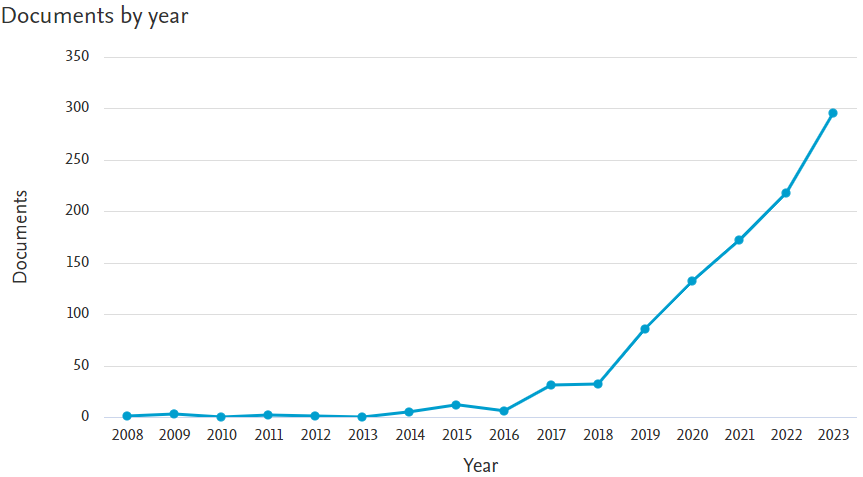
\includegraphics[width=1\textwidth]{Plantilla_TFG_latex//imagenes//Inf//EdA/scopus_mh.png}}
  \hfill
  \subfloat{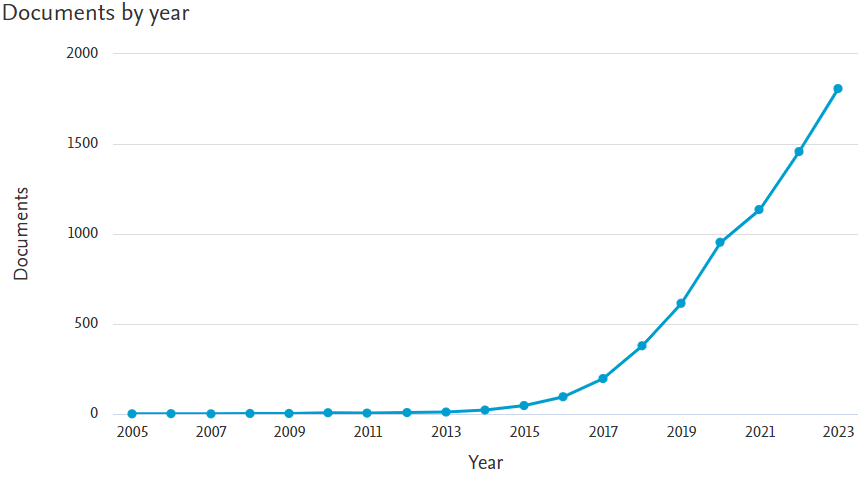
\includegraphics[width=1\textwidth]{Plantilla_TFG_latex//imagenes//Inf//EdA/scopus_gd.png}}
  \caption[Número de documentos indexados anualmente en la base de datos Scopus relacionados con el entrenamiento de modelos de aprendizaje profundo mediante diferentes enfoques]{Número de documentos indexados anualmente en la base de datos Scopus relacionados con el entrenamiento de modelos de aprendizaje profundo mediante diferentes enfoques. La primera gráfica (arriba) muestra la cantidad de artículos que exploran el uso de MH para la optimización del entrenamiento de redes neuronales profundas, obteniendo un total de 997 publicaciones. La segunda gráfica (abajo) presenta el volumen de publicaciones centradas en el entrenamiento basado en GD, obteniendo un total de 6,753, lo que resulta en una diferencia de 7 veces mayor. Se observa que, si bien ambos enfoques han ganado interés en los últimos años, el uso de GD domina ampliamente la producción científica, con un crecimiento exponencial en el número de publicaciones desde 2017. La búsqueda se realiza a fecha del 11 de noviembre de 2024.}
  \label{fig:resEdA}
\end{figure}

Obtenemos una cantidad de 6,753 artículos en lo referente al entrenamiento de modelos de aprendizaje profundo con técnicas basadas en GD y 997 para técnicas MH. \textbf{Vemos que la diferencia entre ambas cantidades es considerable, siendo la primera 7 veces mayor que la segunda}. Destacamos sin embargo que la tendencia en ambos casos es muy similar, como se observa en la Figura \ref{fig:resEdA}, aumentando prácticamente en la misma proporción desde el año 2012.



\subsection{Gradiente descendente y optimizadores}

\textbf{El GD es el algoritmo de aprendizaje utilizado por defecto en prácticamente todas las tareas de aprendizaje profundo, gracias a su eficiencia y buenos resultados}. Los problemas que surgen en su convergencia se intentan evitar en la práctica mediante el desarrollo de modificaciones a su algoritmo, denominadas optimizadores. La literatura en este ámbito es extensa, con una gran variedad de ellos disponibles. A continuación, realizaremos una distinción clara entre optimizadores de primer y de segundo orden.


Aunque los optimizadores de segundo orden presentan mejores propiedades teóricas y ofrecen una convergencia más rápida y estable al utilizar más información del problema, el cálculo o la aproximación de la matriz Hessiana incrementa significativamente el poder computacional necesario para su uso, lo que ralentiza el entrenamiento. Además, hay un problema de memoria: para una red neuronal con 1 millón de parámetros, se requeriría almacenar una matriz de tamaño $1,000,000 \times 1,000,000$, que ocuparía aproximadamente 3,725 GB de memoria RAM. Esto resulta inviable, especialmente considerando que en el top-10 de modelos de clasificación de la competición \textit{ImageNet}, ningún modelo tiene menos de mil millones de parámetros.

Incluso si eliminamos estos inconvenientes de memoria con métodos como L-BFGS (ver Sección \ref{sec:l-bfgs}), enfrentamos un problema significativo: estos métodos requieren el cálculo del gradiente sobre todos los datos de entrenamiento. Conjuntos como \textit{ImageNet}, que contienen más de un millón de ejemplos, hacen que esto sea computacionalmente inviable. Conseguir que este tipo de algoritmos como L-BFGS funcionen con \textit{batches} es más complejo que en MBGD y de hecho es un área abierta de investigación.

En la práctica no es común ver el algoritmo L-BFGS u otros optimizadores de segundo orden aplicados a modelos de aprendizaje profundo a gran escala. En su lugar se utilizan variantes de MBGD basadas en el uso de momento y en tasas de aprendizaje adaptativas, ya que son mucho más simples y más escalables. Existen varias opciones bastante asentadas, que forman parte de las librerías de aprendizaje automático más usadas como PyTorch y TensorFlow, entre las cuales destacan Adam, NAG, RMSProp, AdaGrad o SGD con momento. Vamos a analizar la comparativa \cite{Kyrillidis2020} entre los optimizadores basados en GD con rendimiento del estado del arte para obtener una visión general.

En ella se diferencia entre los algoritmos que tienen tasa de aprendizaje adaptativa (Adam, AMSGrad, AdamW, QHAdam, Demon Adam, YellowFin) y los que no (SGDM, AggMo, QHM, Demon Momentum). Una consideración muy importante que se realiza en dicha comparativa, y que es bien sabida en el campo del aprendizaje automático, es que el rendimiento de una técnica de entrenamiento está muy ligado al dominio específico del problema. Puede ocurrir que un método que no sea de los mejores en términos generales sí lo sea en un problema específico. Pasamos ahora a describir rápidamente las técnicas más interesantes.


YellowFin \cite{yellowfin} es un optimizador con tasa de aprendizaje y momento adaptativos, de manera que mantiene dichos hiperparámetros en un intervalo donde el ratio de convergencia es una constante igual a la raíz del momento. AdamW es una extensión de Adam en la que se utiliza penalización en los pesos del modelo de manera que exista un sesgo hacia valores más pequeños de los mismos durante el entrenamiento, ya que normalmente se asocian valores grandes en los parámetros con el sobreajuste. Aunque Adam ya incorpora este mecanismo, AdamW realiza una pequeña modificación a través de desacoplar esta penalización de la actualización del gradiente, resultando en un impacto notable. 

QHM es una extensión del método de momento clásico que introduce un término cuasi-hiperbólico. Esto permite una mezcla controlada entre el momento y el algoritmo de GD original, proporcionando una mayor flexibilidad y mejorando la estabilidad del entrenamiento. QHAdam combina las ventajas del optimizador Adam con las del GD con momento cuasi-hiperbólico. Introduce factores de amortiguación para controlar la contribución de las medias móviles de primer y segundo orden, ofreciendo un equilibrio entre estabilidad y rapidez en la convergencia. 

Demon Adam es una variante de Adam que ajusta dinámicamente el momento durante el entrenamiento. Utiliza una estrategia de decaimiento del momento para mejorar la adaptación a diferentes fases del entrenamiento, permitiendo una mejor convergencia y evitando caer en mínimos locales. Similar a Demon Adam, Demon Momentum aplica la técnica de decaimiento del momento, pero se usa con optimizadores basados solo en el momento clásico, no en Adam. Mejora la capacidad de adaptación del optimizador durante el entrenamiento al ajustar el momento de manera dinámica. AggMo combina múltiples trayectorias de momento con diferentes factores de decaimiento. Esto ayuda a mejorar la exploración del espacio de parámetros y a mitigar la dependencia de los hiperparámetros del momento, proporcionando una convergencia más robusta y rápida.


Como conclusión, y atendiendo siempre al dominio específico del problema, se establece que YellowFin es la mejor opción en caso de no disponer de recursos para ajustar los hiperparámetros, ya que adapta el momento y la tasa de aprendizaje a lo largo del entrenamiento. Si se dispone de recursos, pero no demasiados, lo mejor son algoritmos de tasa de aprendizaje adaptativa de manera que sólo se tenga que ajustar el valor del momento; en concreto destacan AdamW, QHAdam y Demon Adam. En cambio si se quiere obtener el mejor rendimiento a toda costa, invirtiendo muchos recursos en el ajuste de parámetros, usar MBGD con momento es la mejor opción, aunque sea un método más clásico.


\subsection{Metaheurísticas en el entrenamiento de modelos}

Aún con el uso de optimizadores, hay ciertos inconvenientes en el entrenamiento que son insalvables, como los que están provocados por los cálculos del gradiente con el algoritmo de \textit{backpropagation}. Las técnicas MH son una gran alternativa, ya que sus operadores de búsqueda no dependen de \textit{backpropagation}, evitando así sus problemas. 

Uno de los enfoques de aplicación de estas técnicas es la combinación con las técnicas clásicas, utilizando diferentes aproximaciones. Por ejemplo en \cite{162} se usa el algoritmo \textit{Artificial Bee Colony} \cite{beesalgo} sobre un conjunto de soluciones aleatorias para generar una población inicial de conjuntos de parámetros de un modelo que se entrenan con GD. En \cite{155} se combina un algoritmo genético con el GD, de manera que las nuevas soluciones son generadas con el operador de búsqueda del primero pero son evaluadas tras realizar varias épocas con el segundo. De manera similar en \cite{163} se usa la técnica MH \textit{Particle Swarm Optimization} \cite{pso} para entrenar los parámetros de la última capa de una ConvNet, mientras que el resto se entrenan a través del algoritmo de GD. La comparación arroja que la hibridación de ambas técnicas alcanza mejores resultados en términos de rapidez de convergencia y de \textit{accuracy}. Prácticamente la totalidad de la literatura referente a esta estrategia está centrada en ConvNets.

Otro enfoque es entrenar el modelo usando exclusivamente algoritmos MH. En este ámbito destacan los estudios \cite{174} y \cite{176}, en los que se proponen dos técnicas basadas en \textit{Simulated Annealing} \cite{siman} para entrenar los parámetros de una ConvNet, consiguiendo mejor rendimiento y mayor velocidad de convergencia que en el mismo modelo entrenado mediante el algoritmo de GD. Al igual que ocurre con el enfoque anterior, la gran mayoría de estos estudios están centrados en ConvNets y \textit{Recurrent Neural Networks}. 

Algo importante a destacar en la literatura de entrenamiento de modelos con técnicas MH es la falta de un marco común en los estudios, lo que impide realizar comparaciones objetivas entre ellos. Esta cuestión, comentada con más detalle en la Sección \ref{sec:motinfo}, evidencia la necesidad de más experimentos bajo condiciones similares para poder sacar conclusiones objetivas entre ellos.

\textbf{El rendimiento de estas técnicas todavía no es comparable al de las técnicas clásicas. Si bien es cierto que para tareas sencillas y modelos con pocos parámetros pueden mejorar al GD en la minimización de la función de pérdida, generalmente en términos de generalización su rendimiento es inferior. Además, es importante considerar la complejidad computacional: para alcanzar un rendimiento similar al del GD, estas técnicas requieren mucho más tiempo y recursos computacionales, por lo que no resultan una alternativa viable para este tipo de tareas.}






\subsection{Neuroevolución}

La neuroevolución es un enfoque que combina algoritmos evolutivos con redes neuronales, con el objetivo de optimizar sus pesos, arquitecturas o reglas de aprendizaje \cite{Yao1999}. A diferencia de los métodos de optimización basados en gradiente, la neuroevolución utiliza principios inspirados en la evolución biológica para desarrollar y entrenar redes neuronales, ofreciendo alternativas robustas especialmente en escenarios donde el cálculo de gradientes resulta complejo o inviable.



El paradigma de la neuroevolución se basa en la aplicación de operadores evolutivos (selección, cruce y mutación) para desarrollar redes neuronales, sin depender de información de gradiente. \cite{Whitley1990} establecieron algunas de las bases iniciales al demostrar cómo los algoritmos genéticos podían optimizar tanto las conexiones como la conectividad en redes neuronales. Este enfoque resulta particularmente valioso en problemas con espacios de búsqueda no diferenciables, funciones objetivo ruidosas o con múltiples óptimos locales \cite{Stanley2019}. La neuroevolución puede aplicarse a diferentes aspectos de las redes neuronales:

\begin{itemize}
    \item Optimización de pesos: evolucionamos los parámetros del modelo.
    \item Evolución de arquitecturas: donde la topología de la red (número de capas, neuronas y conexiones) es determinada evolutivamente.
    \item Evolución de reglas de aprendizaje: donde los propios algoritmos de aprendizaje son evolucionados.
\end{itemize}




El algoritmo \textit{NeuroEvolution of Augmenting Topologies} (NEAT), propuesto por \cite{Stanley2002}, representa uno de los avances más significativos en neuroevolución. NEAT permite la evolución simultánea de la topología y los pesos de las redes neuronales, comenzando con estructuras mínimas que gradualmente se vuelven más complejas. Este enfoque ha demostrado capacidad para generar soluciones más compactas y eficientes que otros métodos neuroevolutivos convencionales. Sus características distintivas incluyen:

\begin{enumerate}
    \item Operadores de mutación que pueden añadir nodos y conexiones.
    \item Un sistema de marcado histórico que resuelve el problema de cruzamiento entre redes con diferentes topologías.
    \item Especiación para asegurar innovaciones estructurales.
\end{enumerate}





Con el auge del aprendizaje profundo, la investigación ha evolucionado hacia la aplicación de técnicas evolutivas en redes neuronales de múltiples capas. \cite{David2014} presentaron un enfoque para evolucionar redes neuronales profundas mediante algoritmos genéticos, demostrando su viabilidad en problemas de clasificación. \cite{Such2017} ampliaron este campo al demostrar que los algoritmos genéticos constituyen una alternativa competitiva frente a métodos como el aprendizaje por refuerzo profundo. Su investigación reveló que la simple búsqueda de mutaciones en el espacio de pesos de redes neuronales puede superar a algoritmos complejos basados en gradiente en ciertas tareas de refuerzo. 



La neuroevolución ha encontrado aplicaciones en diversas áreas:



\begin{enumerate}
    \item \textbf{Aprendizaje por refuerzo}: Donde la ausencia de gradientes claros dificulta los métodos tradicionales. \cite{Miikkulainen2019} demostraron la eficacia de la neuroevolución en entornos de aprendizaje por refuerzo complejos.

    \item \textbf{Redes neuronales de impulsos (\textit{Spiking Neural Networks})}: \cite{Pavlidis2005} aplicaron algoritmos evolutivos para entrenar este tipo de redes, donde los métodos basados en gradiente resultan particularmente difíciles de implementar debido a la naturaleza discontinua de los impulsos neuronales.

    \item \textbf{Problemas con funciones objetivo no diferenciables}: La neuroevolución permite optimizar redes neuronales respecto a criterios que no proporcionan gradientes, como métricas discretas o comportamientos emergentes complejos.
\end{enumerate}


En artículos recientes, \cite{Stanley2019} sugieren que el futuro de la neuroevolución reside en su capacidad para descubrir arquitecturas novedosas y adaptativas, complementando más que compitiendo con los métodos basados en gradiente. Esta visión híbrida podría conducir a sistemas que combinen la eficiencia local del GD con la exploración global de los métodos evolutivos. En \cite{Slowik2008} se demuestra cómo los algoritmos de evolución diferencial pueden complementar los métodos tradicionales de entrenamiento, ofreciendo mejoras significativas en términos de tiempo de convergencia y calidad de las soluciones. La revisión comprehensiva de \cite{Kaveh2023} sobre algoritmos MH para el entrenamiento de redes neuronales confirma esta tendencia hacia enfoques híbridos, donde la neuroevolución juega un papel fundamental en la optimización global del proceso de aprendizaje, mientras que los métodos basados en gradiente se encargan del refinamiento local.



\subsection{Aprendizaje Automático Automatizado}

El Aprendizaje Automático Automatizado (AutoML) emerge como una respuesta a la creciente complejidad y especialización requerida en el desarrollo de modelos de aprendizaje automático. Esta disciplina busca automatizar el proceso de selección, configuración y optimización de modelos, reduciendo la necesidad de intervención humana especializada y democratizando el acceso a técnicas avanzadas de aprendizaje automático \cite{Hutter2019}.

Esta automatización se fundamenta en métodos de búsqueda y optimización que evalúan iterativamente diferentes configuraciones, buscando maximizar métricas de rendimiento definidas \cite{Hutter2019}. La relación entre AutoML y las MH es estrecha, ya que muchas técnicas de AutoML utilizan algoritmos evolutivos, búsqueda bayesiana u otros métodos MH como motores de optimización \cite{Kaveh2023}.

La optimización bayesiana constituye uno de los enfoques más utilizados en AutoML, modelando la función objetivo (el rendimiento del modelo) como un proceso gaussiano y utilizando técnicas de adquisición para seleccionar puntos de evaluación prometedores. Este enfoque permite balancear eficientemente la exploración y explotación en el espacio de hiperparámetros \cite{Shahriari2016}.


Los algoritmos evolutivos ofrecen una alternativa robusta para la optimización en AutoML. En \cite{Alba2006} documentan cómo diversos procedimientos MH, incluyendo algoritmos genéticos y evolución diferencial, pueden aplicarse efectivamente al entrenamiento y configuración de redes neuronales. Estos métodos resultan particularmente valiosos para espacios de búsqueda complejos y no diferenciables.

\cite{Miikkulainen2019} proponen la evolución de redes neuronales profundas completas, incluyendo tanto arquitecturas como hiperparámetros, demostrando que los métodos evolutivos pueden generar soluciones competitivas para problemas complejos de aprendizaje automático.


Los algoritmos de \textit{multi-armed bandit} y sus variantes permiten la asignación dinámica de recursos computacionales a configuraciones prometedoras, descartando eficientemente opciones subóptimas. Estos métodos han sido implementados en sistemas como \textit{Hyperband} \cite{Li2018}, que combina la búsqueda aleatoria con una estrategia de asignación de recursos basada en \textit{bandits}.

Aunque AutoML busca reducir la necesidad de experiencia humana, la integración efectiva de conocimiento experto en el proceso automatizado representa un área de investigación prometedora. Los enfoques que permiten a los expertos guiar el proceso de búsqueda o incorporar restricciones específicas del dominio podrían mejorar significativamente la efectividad de los sistemas AutoML \cite{Hutter2019}. Las direcciones futuras apuntan hacia sistemas más integrados que combinen diferentes enfoques de optimización, aprovechando tanto métodos basados en gradiente como MH evolutivas, y que puedan adaptarse dinámicamente a los requisitos específicos de cada problema \cite{Elsken2019}.












\subsection{Búsqueda de Arquitectura Neuronal}

Búsqueda de Arquitectura Neuronal (NAS, por sus siglas en inglés, \textit{Neural Architecture Seach}) representa un subcampo especializado dentro del AutoML, centrado específicamente en la automatización del diseño de arquitecturas de redes neuronales. Esta disciplina busca sustituir el proceso manual de diseño arquitectónico por metodologías algorítmicas que puedan descubrir estructuras óptimas o casi óptimas para problemas específicos \cite{Elsken2019}. El diseño manual de arquitecturas neuronales ha sido tradicionalmente un proceso que requiere considerable experiencia y conocimiento especializado, además de seguir un ciclo iterativo de prueba y error. Esta complejidad ha motivado el desarrollo de métodos automáticos que puedan explorar sistemáticamente el espacio de arquitecturas posibles \cite{Zoph2017}.


Los métodos de NAS pueden clasificarse en tres grupos: basados en aprendizaje por refuerzo, evolutivos y basados en gradiente. Los primeros formulan el diseño arquitectónico como un problema de decisión secuencial, donde un agente aprende a seleccionar componentes arquitectónicos que maximizan métricas de rendimiento. El trabajo pionero de \cite{Zoph2017} demostró la viabilidad de este enfoque, utilizando redes neuronales recurrentes como controladores para generar descripciones de arquitecturas.

Los algoritmos evolutivos constituyen una alternativa robusta para NAS, al modelar las arquitecturas como individuos dentro de una población que evoluciona mediante operadores genéticos. Un ejemplo destacado de este enfoque es el trabajo de Xie et al., quienes propusieron un método basado en algoritmos genéticos para evolucionar arquitecturas de redes convolucionales, logrando resultados competitivos en tareas de clasificación de imágenes \cite{Xie2017}. Posteriormente, Lu et al. ampliaron este enfoque con NSGA-Net, un algoritmo genético multiobjetivo diseñado para optimizar de manera simultánea la precisión y la complejidad computacional de las arquitecturas \cite{Lu2018}. Este trabajo evidencia cómo los métodos evolutivos pueden abordar de manera eficaz la naturaleza multiobjetivo inherente al diseño de arquitecturas neuronales. Por otro lado, Stanley et al. destacan las ventajas de la neuroevolución en el contexto de NAS, subrayando su capacidad para explorar de forma eficiente espacios de búsqueda complejos y no diferenciables \cite{Stanley2019}. En esta línea, el algoritmo NEAT, desarrollado por Stanley y Miikkulainen, ofrece un marco natural para la evolución de topologías neuronales, lo que lo convierte en una estrategia adecuada para la búsqueda automatizada de arquitecturas \cite{Stanley2002}.




A diferencia de los enfoques anteriores, los métodos basados en gradiente relajan el problema discreto de selección arquitectónica a un problema continuo, permitiendo la aplicación de técnicas de optimización basadas en gradiente. DARTS (\textit{Differentiable Architecture Search}) ejemplifica este enfoque, utilizando relajaciones \textit{softmax} para hacer diferenciable el proceso de selección de operaciones \cite{Liu2018}.



La principal limitación de NAS es su coste computacional, lo que ha motivado diversas estrategias para mejorar su eficiencia, como compartir pesos entre las distintas arquitecturas candidatas \cite{Pham2018} en ENAS (\textit{Efficient Neural Architecture Search}), usar tareas simplificadas o predictores de rendimiento para ahorrar coste computacional \cite{Baker2018}, o descomposición jerárquica del problema en otros más pequeños (entrenar partes de la arquitectura por separado y luego combinarlas) \cite{Miikkulainen2019,Liu2018}.


Los estudios comparativos entre arquitecturas generadas automáticamente y diseñadas manualmente han arrojado resultados significativos:

\begin{enumerate}
\item \textbf{Rendimiento}: En diversas tareas, las arquitecturas generadas mediante NAS han igualado o superado a las diseñadas manualmente. Por ejemplo, NASNet \cite{Zoph2018} superó el rendimiento de ResNet e Inception en tareas de clasificación de imágenes.

\item \textbf{Eficiencia computacional}: Mediante optimización multiobjetivo, como en NSGA-Net \cite{Lu2018}, es posible generar arquitecturas que balancean precisión y eficiencia computacional, superando a modelos manuales en ambas dimensiones.

\item \textbf{Transferibilidad}: Las arquitecturas descubiertas en tareas específicas han demostrado buena capacidad de transferencia a otras tareas relacionadas, sugiriendo que NAS puede identificar estructuras con propiedades generalizables \cite{Lu2018}.

\item \textbf{Novedad estructural}: Los métodos de NAS han descubierto estructuras novedosas que difieren significativamente de los diseños convencionales, como conexiones densas no intuitivas o patrones de conexión irregulares \cite{Real2019}.
\end{enumerate}



La adaptación de NAS a dominios específicos como redes neuronales recurrentes, redes generativas adversarias o redes de grafos representa un área de investigación activa \cite{Gao2020}. La integración de NAS con otros componentes del ciclo de aprendizaje automático, como la selección de características o la optimización de hiperparámetros, apunta hacia sistemas más comprensivos que puedan optimizar \textit{pipelines} completos de aprendizaje automático \cite{Kaveh2023}. La evolución de NAS refleja una tendencia más amplia hacia la automatización del diseño de sistemas de aprendizaje automático, donde los métodos evolutivos y otras MH juegan un papel fundamental al proporcionar marcos robustos para la exploración de espacios de diseño complejos y no diferenciables.






\section{Experimentación}

Se ha desarrollado una batería de pruebas amplia y diversa que permita una correcta comparación entre el gradiente descendente y las técnicas metaheurísticas atendiendo a los objetivos señalados anteriormente. En la tabla \ref{table:exp} se ofrece un resumen esquemático de las pruebas que se van a realizar. Todas ellas se realizan con los siguientes optimizadores de gradiente descendente: NAG, RMSProp y Adam. Para las metaheurísticas se ha elegido los ya conocidos en la literatura SHADE y SHADE-ILS, y añadiendo una versión híbrida de cada uno con el gradiente descendente. Todas estas elecciones se detallarán a lo largo de esta sección. Para el desarrollo del código se usa el lenguaje Python con las librerías PyTorch y FastAI, entre otras; implementado y ejecutado en Google Colab. El código puede encontrarse en: https://github.com/eedduu/TFG.




\begin{table}[]
\begin{tabular}{|l|cccc|cll|}
\hline
\textbf{Familia} & \multicolumn{4}{c|}{MLP}                                                                                                                               & \multicolumn{3}{c|}{ConvNets}                                         \\ \hline
\textbf{Modelo}  & \multicolumn{4}{c|}{1,2,5 y 11}                                                                                                                        & \multicolumn{3}{c|}{LeNet5, ResNet-15 y ResNet57}                               \\ \hline
\textbf{Datasets}           & \multicolumn{1}{c|}{BHP} & \multicolumn{1}{c|}{BCW} & \multicolumn{2}{c|}{WQ}              & \multicolumn{1}{c|}{MNIST} & \multicolumn{1}{l|}{F-MNIST} & CIFAR10-G \\ \hline
\textbf{Tarea}             & \multicolumn{1}{c|}{R}                        & \multicolumn{1}{c|}{C}            & \multicolumn{1}{c|}{R} & C & \multicolumn{3}{c|}{Clasificación de imágenes}                        \\ \hline
\end{tabular}
\caption{Resumen de la experimentación. BHP: Boston Housing Price, BCW: Breast Cancer Winsconsin, WQ: Wine Quality. R: regresión, C: clasificación. En el caso de MLP, en la fila modelo se indica el número de capas ocultas.}
\label{table:exp}
\end{table}

\subsection{Modelos}

Usaremos dos familias de modelos: MLP y ConvNets. Con los primeros usaremos datasets tabulares para clasificación y regresión, y con los segundos datasets de imágenes para la tarea de clasificación. En la siguiente sección se detallan los datasets con sus características.

La implementación de los MLP se ha realizado a través de la librería FastAI por simplicidad ya que ofrece lo necesario para usarlos directamente. La implementación de las ConvNets se ha realizado desde cero, observando la topología de LeNet5 y las ResNets en sus papers originales, ya que en ellas sí que se han introducido ciertos cambios que se comentan más adelante. Estas modificaciones tienen como objetivo una batería experimental más amplia y acorde a las condiciones que buscamos. Todos los modelos han sido entrenados desde cero.

Para los MLP usaremos 5 modelos, con 1,2,5 y 11 capas ocultas cada uno. El número de neuronas por capa es una potencia de 2 y con estructura piramidal incremental, es decir primero aumentando el número de neuronas por capa y luego disminuyéndolo. Estas son elecciones comunes en la literatura ya que facilitan las operaciones por su estructura (la primera) y el tratamiento de los datos (la segunda). El objetivo es conseguir una variedad experimental que permita medir los efectos de la complejidad del modelo sobre la tarea y el overfitting además de adecuarse a las condiciones del paper de referencia, con modelos desde aproximadamente mil parámetros hasta casi 1.5M como vemos en \ref{tab:MLPmod}, acercándose al modelo más grande presentado en dicho paper. 

\begin{table}[]
\centering
\begin{tabular}{|c|c|c|}
\hline
\textbf{Capas ocultas} & \textbf{Neuronas por capa}                                                                     & \textbf{Parámetros} \\ \hline
1                      & 64                                                                                             & 2238                \\ \hline
2                      & 64, 64                                                                                         & 6462                \\ \hline
5                      & 64, 128, 256, 128, 64                                                                          & 85k                 \\ \hline
11                     & \begin{tabular}[c]{@{}c@{}}32, 64, 128, 256, 512, 1024, \\ 512, 256, 128, 64 y 32\end{tabular} & 1.4M                \\ \hline
\end{tabular}
\caption{Detalles de los modelos MLP}
\label{tab:MLPmod}
\end{table}

Antes de cada capa linal hay una de BatchNorm1D, ya que es la implementación por defecto de FastAI y mejora el rendimiento en el entrenamiento. Los parámetros asociados a este tipo de capa y a los de la capa de salida van incluidos en el cómputo anterior. Se incluye al final del modelo una capa de SoftMax en caso de que la tarea sea clasificación.

Para los modelos basados en convoluciones usamos LeNet5 y dos ResNets, con 15 y 57 capas. El objetivo es de nuevo ofrecer una variedad experimental, con el primer modelo teniendo unos 60k parámetros mientras que el tercero tiene 1.3M, imitando de nuevo las condiciones del paper de referencia. Hay que resaltar que la intención es comparar varios modelos con diferente número de parámetros para ver el efecto sobre éstos, y no hablamos de modelos más o menos potentes, ya que no siempre un incremento en el número de parámetros se traduce en un mejor rendimiento.


LeNet5 es un modelo de sobra conocido presentado por Yann LeCun en \cite{lenet5}, al que sustituimos las funciones de activación por ReLU, ya que en la literatura posterior a la presentación del modelo se han demostrado superiores a las sigmoides y la tangente hiperbólica. También se han sustituido las capas de AveragePool por MaxPool y añadido capas de BatchNorm por los mismos motivos. En la tabla \ref{table:lenet5} se muestra la topología de este modelo, obviando las capas de Flatten y de SoftMax. Tiene un total de 62 mil parámetros.



\begin{table}[]
\centering
\begin{tabular}{|c|c|c|c|}
\hline
\multirow{2}{*}{\textbf{Capa}} & \multirow{2}{*}{\textbf{Dimensión}} & \multirow{2}{*}{\textbf{Kernel}} & \multirow{2}{*}{\textbf{Canales}} \\
                               &                                     &                                  &                                   \\ \hline
Convolución                    & 28x28                               & 5x5                              & 6                                 \\ \hline
BatchNorm2D                    & 28x28                               & -                                & -                                 \\ \hline
ReLU                           & 28x28                               & -                                & -                                 \\ \hline
Max Pool                       & 14x14                               & 2x2, stride 2                    & -                                 \\ \hline
Convolución                    & 10x10                               & 5x5                              & 16                                \\ \hline
BatchNorm2D                    & 10x10                               & -                                & -                                 \\ \hline
ReLU                           & 10x10                               & -                                & -                                 \\ \hline
Max Pooling                    & 5x5                                 & 2x2                              & -                                 \\ \hline
Lineal                         & 120                                 & -                                & -                                 \\ \hline
BatchNorm1D                    & 120                                 & -                                & -                                 \\ \hline
ReLU                           & 120                                 & -                                & -                                 \\ \hline
Lineal                         & 84                                  & -                                & -                                 \\ \hline
BatchNorm1D                    & 84                                  & -                                & -                                 \\ \hline
ReLU                           & 84                                  & -                                & -                                 \\ \hline
Lineal                         & num\_classes                        & -                                & -                                 \\ \hline
\end{tabular}
\caption{Topología de LeNet5 para imágenes 32x32 con un canal de entrada. Las columnas dimensión y canales hacen referencia a la salida de la capa.}
\label{table:lenet5}
\end{table}


Se han diseñado dos modelos de ResNet, uno con 15 capas y otro con 57. A priori puede parecer excesivo 57 capas, pero con la implementación a través de BottleNeckBlocks se aumenta el número de capas considerablemente con un leve incremento del número de parámetros. Sigue además la tendencia en la literatura de aumentar el número de capas antes que el número de filtros. Se han elegido 57 capas con la intención de aproximarse al número de parámetros del modelo más grande del paper de referencia y aprovechar la estructura de esta familia de modelos. Las ResNets se caracterizan por usar bloques convolucionales que agrupan varias capas de convolución donde al final de cada bloque se suma la entrada del mismo, con el objetivo de evitar el problema del desvanecimiento de gradiente (ver sección \ref{sec:desvyexpl}). En un modelo con pocas capas no se aprecia tan bien este efecto. Su topología se detalla en la tabla \ref{table:resnet57}.

El modelo intermedio, Resnet15, sigue la misma estructura que ResNet57 pero usando menos bloques convolucionales. El objetivo es tener un modelo intermedio, con unos 500 mil parámetros y que nos permita comparar con los otros dos, en términos de entrenamiento y de overfitting, algo muy usual en las redes neuronales con gran número de parámetros.  Su topología se detalla en la tabla \ref{table:resnet15}.

Los bloques convolucionales agrupan 3 capas de convolución con sus respectivas capas BatchNorm, y se usan convoluciones 1x1 para hacer cuello de botella, reduciendo así el número de parámetros sin perder expresividad de la red \cite{bottleorig, bottlegoogle}. Se sigue el diseño usual de esta familia de modelos, por ejemplo agrupando más bloques convolucionales en mitad de la red, con una convolución preia a los bloques convolucionales y usando solo una capa lineal. El modelo ResNet57 que se implementa tiene un total de 1.3M de parámetros. 

\begin{table}[]
\begin{tabular}{|c|c|c|c|}
\hline
\multirow{2}{*}{\textbf{Capa}} & \multirow{2}{*}{\textbf{Dimensión}} & \multirow{2}{*}{\textbf{Kernel/Stride}} & \multirow{2}{*}{\textbf{Canales}} \\
                               &                                            &                                         &                                          \\ \hline
Convolución                    & 26x26                                      & 7x7                                     & 64                                       \\ \hline
BatchNorm2d                    & 26x26                                      & -                                       & -                                        \\ \hline
ReLU                           & 26x26                                      & -                                       & -                                        \\ \hline
MaxPool2d                      & 13x13                                      & 2x2, stride 2, padding 1                & -                                        \\ \hline
BottleneckBlock x3             & 13x13                                      & 1x1, 3x3, 1x1                           & 64                                       \\ \hline
BottleneckBlock x4             & 7x7                                        & 1x1, 3x3, 1x1, stride 2                 & 128                                      \\ \hline
BottleneckBlock x4             & 4x4                                        & 1x1, 3x3, 1x1, stride 2                 & 256                                      \\ \hline
BottleneckBlock x3             & 2x2                                        & 1x1, 3x3, 1x1, stride 2                 & 512                                      \\ \hline
AdaptiveAvgPool2d              & 512                                        & -                                       & -                                        \\ \hline
BatchNorm1d                    & 512                                        & -                                       & -                                        \\ \hline
Dropout                        & 512                                        & -                                       & -                                        \\ \hline
Lineal                         & num\_classes                               & -                                       & -                                        \\ \hline
\end{tabular}
\caption{Topología de ResNet57 para imágenes 32x32 con un canal de entrada. Las columnas dimensión y canales hacen referencia a la salida de la capa.}
\label{table:resnet57}
\end{table}


\begin{table}[]
\begin{tabular}{|c|c|c|c|}
\hline
\multirow{2}{*}{\textbf{Capa}} & \multirow{2}{*}{\textbf{Dimensión}} & \multirow{2}{*}{\textbf{Kernel/Stride}} & \multirow{2}{*}{\textbf{Canales}} \\
                               &                                     &                                         &                                   \\ \hline
Convolución                    & 26x26                               & 7x7                                     & 64                                \\ \hline
BatchNorm2d                    & 26x26                               & -                                       & -                                 \\ \hline
ReLU                           & 26x26                               & -                                       & -                                 \\ \hline
MaxPool2d                      & 13x13                               & 2x2, stride 2, padding 1                & -                                 \\ \hline
BottleneckBlock x1             & 13x13                               & 1x1, 3x3, 1x1                           & 64                                \\ \hline
BottleneckBlock x1             & 7x7                                 & 1x1, 3x3, 1x1, stride 2                 & 128                               \\ \hline
BottleneckBlock x1             & 4x4                                 & 1x1, 3x3, 1x1, stride 2                 & 256                               \\ \hline
BottleneckBlock x1             & 2x2                                 & 1x1, 3x3, 1x1, stride 2                 & 512                               \\ \hline
AdaptiveAvgPool2d              & 512                                 & -                                       & -                                 \\ \hline
BatchNorm1d                    & 512                                 & -                                       & -                                 \\ \hline
Dropout                        & 512                                 & -                                       & -                                 \\ \hline
Lineal                         & num\_classes                        & -                                       & -                                 \\ \hline
\end{tabular}
\caption{Topología de ResNet15 para imágenes 32x32 con un canal de entrada. Las columnas dimensión y canales hacen referencia a la salida de la capa.}
\label{table:resnet15}
\end{table}






\subsection{Datasets}

TODO: añadir información sobre los datasets: número de características, target, tamaño, qué contienen, imagenes.

\subsubsection{Tabulares}

BCW y WQ para clasificación, BHP y WQ para regresión. El objetivo es comparar también el rendimiento de las metaheurísticas en estas tareas, ya que la gran mayoría de la literatura sobre MH se realiza con ConvNets y por tanto con tareas de clasificación. BCW y BHP son dos dataset pequeños (alrededor de 500 instancias) y más fáciles que WQ, que tiene una cantidad de unas 6000 instancias. Por ello hay una tarea sencilla y una difícil para regresión y clasificación.

Para estos datasets se ha realizado un preprocesado de los datos básico y con decisiones comunes basadas en la literatura. Se han eliminado las variables que tienen menos de un 5 o 10\% (dependiendo de la cantidad de variables del dataset) de correlación con el target. Con las parejas de variables que tienen más de un 90\% de correlación entre sí se elimina una de las dos. Se han eliminado outliers con el método zscore usando un threshold de 3 y se han normalizado los datos de entrada.

El tamaño del batch se ha elegido mediante pruebas experimentales entre los valores 32, 64 y 128. Se divide el conjunto de datos en entrenamiento-validación-test, con un porcentaje 70-10-20.



\subsubsection{Imágenes}

Para los datasets de imágenes se han elegido tres de los usados en el paper de referencia. Se han elegido MNIST y FMNIST ya que son los más usados para la comparativa en dicho paper, y CIFAR10 ya que a priori es más difícil que los otros, siendo MNIST el más fácil de los tres. Esto proporciona unas pruebas equilibradas, en el mismo marco que el paper y permite una fácil comparación. Al igual que allí, se ha reducido el tamaño de los datasets a 10 mil imágenes para el entrenamiento y 5 mil para el test. Del conjunto de entrenamiento se toma el 30\% para validación.

Se usan las imágenes con una resolución de 32x32 y un solo canal, adaptando las imágenes a estas dimensiones cuando sea necesario. No se usa preprocesamiento de datos ya que se entiende que la propia red a través de las convoluciones los procesa.


\subsection{Otras decisiones}

Para la reproducibilidad de la experimentación, se fija la semilla 42 en todos las librerías necesarias. No se usa cross validation debido a que las técnicas metaheuristicas requieren de mucho más poder de cómputo que el disponible para poder ejecutarlas varias veces en un tiempo razonable.

Se ha usado la inicialización de pesos Glorot  como en el paper a comparar. Para los optimizadores basados en gradiente descendente se han usado los mismos pesos iniciales, mientras que en las técnicas metaheurísticas se ha usado la misma población inicial, para asegurar la igualdad de condiciones en el entrenamiento debido a la gran sensibilidad de éste a los parámetros iniciales. 

Se fija 20 como número de épocas en todos los entrenamientos ya que es suficiente para la convergencia de los métodos de gradiente descendente. Siguiendo el criterio del paper de referencia, en las técnicas metaheurísticas una época es algo distinta, siendo en el paper equivalente a $N_eval * N_epochs * N_capas$. En nuestro caso no se ha usado el factor número de capas por diversas razones: no se realiza entrenamiento individualizado por capas, no se dispone de tanto poder de cómputo, usamos modelos con muchas capas. Aunque usemos menos evaluaciones del conjunto de entrenamiento por época, la comparación sigue en la misma dinámica y las metaheurísticas recibirán mucho más poder de procesamiento que las técnicas clásicas.

Para las tareas de regresión se ha usado el error cuadrático medio como función de coste. Es ampliamente usada en la literatura y aunque es sensible a los outliers, como tenemos preprocesamiento de datos no nos afecta. Se ha usado también la métrica R2 cuadrado para medir la explicación de la varianza con respecto a la media como predicción, para tener un criterio objetivo de comparación ya que en las dos tareas de regresión la escala del objetivo es distinta. Para las tareas de clasificación se ha usado CrossEntropyLoss como función de error y accuracy como métrica, opciones ampliamente usadas en la literatura. En los datasets tabulares se ha usado BalancedAccuracy en lugar de Accuracy, ya que las clases no están balanceadas, y se conoce que en estos casos accuracy no es una métrica representativa, de hecho se hace especial mención a esto en el paper. En los datasets de imágenes las clases están perfectamente balanceadas por lo que se usa accuracy, aunque en este caso su versión balanceada coincidiría con la normal.


\subsection{Optimizadores}

Existen tres familias de optimizadores del gradiente descendente principales: las que usan el momento, las que autoajustan el learning rate y las que combinan estas dos estrategias. Para la experimentación se elige un optmizador de cada familia con la intención de ver si existe alguna diferencia en el entrenamiento del gradiente descendente debido a éstos. El criterio para la elección del optimizador de cada familia ha sido el número de citas en el paper de presentación y su extensión de uso, analizando cómo de frecuente es su uso en la literatura y su implementación por defecto en las principales librerías de aprendizaje automático. Respectivamente se han elegido: NAG, RMSProp y Adam.

Se ha usado la implementación de estos optimizadores de PyTorch, usandose en el entrenamiento a través de la librería FastAI. Se usa en el entrenamiento la política de ciclos de Leslie, que proporciona una velocidad de convergencia mucho mayor variando el learning rate de forma cíclica. Para elegir el valor máximo del learning rate se usa un buscador de learning rate, que aporta unos resultados muy buenos a un coste bajo. Cabe destacar que la importancia del learning rate es sensiblemente menor en los optimizadores de RMSProp y Adam, ya que de manera automática ajustan estos valores a lo largo del entrenamiento. 

Para los hiperparámetros de dichos optimizadores se han usado los valores por defecto de la librería PyTorch. En primer lugar, la intención con la experimentación es establecer una comparativa en igualdad de condiciones sobre el entrenamiento de modelos, y no obtener el máximo rendimiento de cada uno. En segundo lugar estos valores por defecto están basados en los propuestos en los respectivos papers originales y ajustados a través de numerosas pruebas experimentales, de manera que proporcionen los mejores resultados posibles de manera general basandose en la propia implementación de PyTorch. 


\subsection{Metaheurísticas}

Para una correcta comparación con el paper de referencia, que usa el algoritmo SHADE-ILS, se eligen 4 algoritmos metaheurísticos entorno a éste. En primer lugar usamos SHADE-ILS, en su versión completa (entrenando todos los parámetros a la vez). Usamos también el algoritmo de SHADE, sin búsqueda local, para usar un algoritmo puramente metaheurístico que no sea memético. Luego estas dos versiones anteriores las hibridamos con el gradiente descendente, para tener algoritmos meméticos que usen información específica del problema. 

El algoritmo de SHADE se implementa a través de la librería pyade-master (LINK), y se le han realizado modificaciones para mantener los parámetros adaptativos del algoritmo SHADE entre ejecuciones distintas y adaptar las estructuras de datos a las del resto del código. A partir de dicho algoritmo se implementan manualmente el resto. Para el algoritmo SHADE-ILS, que combina dos tipos de búsqueda local en su paper original, con una aplicación general, se ha decidido mantener sólo la búsqueda local a través de L-BFGS, ya que al hacer uso del gradiente se maneja información más específica del problema. Esto se realiza a través de la librería scipy.

Se hibridan SHADE y SHADE-ILS con optimizadores basados en gradiente descendente, aunque SHADE-ILS ya usa información del gradiente en su ejecución a través de L-BFGS pero es un optimizador de segundo orden. Para la hibridación se ejecuta el algoritmo y al final de cada 4 épocas se realiza un entrenamiento de gradiente descendente de una época. Esto se realiza para que el peso del entrenamiento lo siga teniendo en mayor medida la parte metaheurística del algoritmo en lugar de la parte clásica. El optimizador que se usa en este caso es el que mejor resultados diera en el entrenamiento basado en gradiente descendente, eligiendo según el modelo que usemos.  

Se mantiene la misma división de los datos que en el uso de optimizadores. Se ejecutan los algoritmos evaluando el error sobre el conjunto de entrenamiento y guardando en cada epoch el mejor individuo de la población junto a su error en el entrenamiento, para luego evaluarlos sobre el conjunto de validación y observar qué modelo generaliza mejor a priori, igual que hacemos en el entrenamiento de modelos con gradiente descendente. Luego evaluamos el modelo sobre el conjunto de test, calculando las métricas asociadas a cada tarea.

Como en el paper de referencia no aparecen los hiperparámetros asociados a estos algoritmos, se decide usar el mismo criterio que con los optimizadores y usar los hiperparámetros por defecto de la implementación de la librería pyade-master, que además son valores comúnes en la literatura. 





\subsection{Experimentos}

\textbf{En esta sección se presentan cuatro experimentos diseñados para evaluar sistemáticamente el rendimiento, eficiencia y aplicabilidad de las MH en comparación con los métodos de GD para el entrenamiento de redes neuronales profundas}. Los experimentos abordan aspectos complementarios que, en conjunto, proporcionan una visión integral del comportamiento de ambos enfoques en diversos escenarios.

\textbf{El primer experimento analiza si existen diferencias estadísticamente significativas en el rendimiento de redes MLP entrenadas con MH según el tipo de tarea} (clasificación vs. regresión). Utilizando conjuntos de datos de complejidad equiparable y aplicando rigurosos tests estadísticos, se evalúa el rendimiento relativo de SHADE-ILS frente a AdamW en ambos tipos de tareas.

\textbf{El segundo experimento profundiza en los factores que más influyen en la pérdida de rendimiento en tareas de clasificación}, tanto en MLPs como en ConvNets. Mediante un análisis de dependencias parciales, se examina cómo la cantidad de ejemplos, la complejidad del conjunto de datos y el número de parámetros del modelo afectan al rendimiento predictivo de los modelos entrenados con ambos tipos de optimizadores (MH y GD).

\textbf{El tercer experimento se centra en analizar los tiempos de ejecución durante el entrenamiento con MH en comparación con el GD}. Este análisis desglosado permite comprender no solo las diferencias absolutas en tiempo, sino también los factores que más impactan en la eficiencia computacional de cada enfoque.

\textbf{Finalmente, el cuarto experimento evalúa el rendimiento de propuestas híbridas propias, específicamente SHADE-GD y SHADE-ILS-GD, que combinan elementos de MH y GD}. Este análisis comparativo determina si estos enfoques híbridos logran capitalizar las fortalezas de ambas técnicas y superar sus limitaciones individuales.




\subsubsection{Experimento 1: Análisis de diferencias en el rendimiento de MLPs entrenados con MH según el tipo de tarea}


\begin{table}[]
\resizebox{\textwidth}{!}{\begin{tabular}{|c|c|ccc|ccc|c|}
\hline
\multirow{2}{*}{Conjunto} & \multirow{2}{*}{Capas} & \multicolumn{3}{c|}{ADAMW}                                        & \multicolumn{3}{c|}{SHADE-ILS}                                         & \multirow{2}{*}{\textbf{Dif$_{rel}$}} \\ \cline{3-8}
                          &                        & \multicolumn{1}{c|}{Train}  & \multicolumn{1}{c|}{Test}  & Metric & \multicolumn{1}{c|}{Train}  & \multicolumn{1}{c|}{Test}   & Metric     &                                       \\ \hline
\multirow{4}{*}{BCW}      & 1                      & \multicolumn{1}{c|}{0.190}  & \multicolumn{1}{c|}{0.108} & 0.960  & \multicolumn{1}{c|}{0.073}  & \multicolumn{1}{c|}{0.142}  & 0.970      & \textbf{0.010}                        \\ \cline{2-9} 
                          & 2                      & \multicolumn{1}{c|}{0.140}  & \multicolumn{1}{c|}{0.041} & 0.980  & \multicolumn{1}{c|}{0.063}  & \multicolumn{1}{c|}{0.350}  & 0.932      & \textbf{-0.049}                       \\ \cline{2-9} 
                          & 5                      & \multicolumn{1}{c|}{0.115}  & \multicolumn{1}{c|}{0.026} & 1.000  & \multicolumn{1}{c|}{0.055}  & \multicolumn{1}{c|}{0.475}  & 0.890      & \textbf{-0.110}                       \\ \cline{2-9} 
                          & 11                     & \multicolumn{1}{c|}{0.112}  & \multicolumn{1}{c|}{0.094} & 0.971  & \multicolumn{1}{c|}{0.098}  & \multicolumn{1}{c|}{0.491}  & 0.903      & \textbf{-0.07}                        \\ \hline
\multirow{4}{*}{WQC}      & 1                      & \multicolumn{1}{c|}{0.970}  & \multicolumn{1}{c|}{2.172} & 0.436  & \multicolumn{1}{c|}{1.098}  & \multicolumn{1}{c|}{1.235}  & 0.201      & \textbf{-0.539}                       \\ \cline{2-9} 
                          & 2                      & \multicolumn{1}{c|}{0.873}  & \multicolumn{1}{c|}{3.177} & 0.500  & \multicolumn{1}{c|}{1.078}  & \multicolumn{1}{c|}{1.340}  & 0.167      & \textbf{-0.666}                       \\ \cline{2-9} 
                          & 5                      & \multicolumn{1}{c|}{0.770}  & \multicolumn{1}{c|}{3.833} & 0.606  & \multicolumn{1}{c|}{0.963}  & \multicolumn{1}{c|}{1.405}  & 0.167      & \textbf{-0.724}                       \\ \cline{2-9} 
                          & 11                     & \multicolumn{1}{c|}{0.940}  & \multicolumn{1}{c|}{3.873} & 0.607  & \multicolumn{1}{c|}{1.137}  & \multicolumn{1}{c|}{1.509}  & 0.167      & \textbf{-0.725}                       \\ \hline
\multirow{4}{*}{WQR}      & 1                      & \multicolumn{1}{c|}{0.475}  & \multicolumn{1}{c|}{0.972} & -0.012 & \multicolumn{1}{c|}{0.611}  & \multicolumn{1}{c|}{0.970}  & -1.988     & \textbf{-164.667}                      \\ \cline{2-9} 
                          & 2                      & \multicolumn{1}{c|}{0.430}  & \multicolumn{1}{c|}{1.126} & 0.072  & \multicolumn{1}{c|}{0.551}  & \multicolumn{1}{c|}{0.826}  & -2.491     & \textbf{-35.597}                      \\ \cline{2-9} 
                          & 5                      & \multicolumn{1}{c|}{0.390}  & \multicolumn{1}{c|}{1.180} & 0.236  & \multicolumn{1}{c|}{0.589}  & \multicolumn{1}{c|}{0.724}  & -983.152   & \textbf{-4166.898}                    \\ \cline{2-9} 
                          & 11                     & \multicolumn{1}{c|}{0.377}  & \multicolumn{1}{c|}{2.162} & 0.133  & \multicolumn{1}{c|}{0.601}  & \multicolumn{1}{c|}{0.734}  & -79529.602 & \textbf{-597967.932}                  \\ \hline
\multirow{4}{*}{BHP}      & 1                      & \multicolumn{1}{c|}{84.429} & \multicolumn{1}{c|}{6.332} & 0.790  & \multicolumn{1}{c|}{10.048} & \multicolumn{1}{c|}{7.549}  & 0.576      & \textbf{-0.271}                       \\ \cline{2-9} 
                          & 2                      & \multicolumn{1}{c|}{55.283} & \multicolumn{1}{c|}{4.577} & 0.832  & \multicolumn{1}{c|}{9.560}  & \multicolumn{1}{c|}{4.648}  & 0.746      & \textbf{-0.103}                       \\ \cline{2-9} 
                          & 5                      & \multicolumn{1}{c|}{94.640} & \multicolumn{1}{c|}{3.511} & 0.847  & \multicolumn{1}{c|}{13.594} & \multicolumn{1}{c|}{14.555} & -0.187     & \textbf{-1.221}                       \\ \cline{2-9} 
                          & 11                     & \multicolumn{1}{c|}{54.540} & \multicolumn{1}{c|}{3.268} & 0.853  & \multicolumn{1}{c|}{43.183} & \multicolumn{1}{c|}{26.794} & -97.404    & \textbf{-115.190}                     \\ \hline
\end{tabular}}
\caption[Resultados del entrenamiento y evaluación de los modelos asociados al primer experimento]{Resultados del entrenamiento y evaluación de los modelos asociados al primer experimento. A partir de estos, intentamos averiguar, a través del test de los rangos con signo de Wilcoxon, si existe una diferencia estadísticamente significativa en el rendimiento de modelos entrenados con MH según el tipo de tarea. Los conjuntos de datos usados son BCW y WQC para clasificación y BHP y WQR para regresión. Estas tareas tienen una complejidad similar dos a dos (BCW-BHP y WQC-WQR). Los MLP, de entre 1 y 11 capas ocultas, son entrenados usando SHADE-ILS como técnica MH y ADAMW como optimizador basado en GD. Como métricas, se usa \textbf{\textit{Balanced Accuracy}} en clasificación y \emph{\textbf{R$^2$}} en regresión. La comparación, realizada de manera relativa observando el rendimiento de los modelos entrenados con MH en relación con su análogo entrenado con GD, no arroja resultados concluyentes.}
\label{tab:exp1}
\end{table}

En este experimento, planteamos la hipótesis de que \textbf{los modelos MLP entrenados con MH presentan diferencias significativas en su rendimiento según el tipo de tarea} (clasificación o regresión). En particular, investigamos si estas diferencias se deben a la naturaleza de la tarea, más que a factores como la complejidad del problema o la arquitectura de la red. Esta hipótesis \textbf{se fundamenta en evidencias experimentales}, como los resultados presentados en la Tabla \ref{tab:exp1}, que sugieren un comportamiento diferenciado en el rendimiento de SHADE-ILS según el tipo de tarea, a diferencia de lo que ocurre con AdamW.

En los conjuntos de datos de clasificación (BCW y WQC), se observa que AdamW tiende a obtener un mejor desempeño en términos de métrica \textit{Balanced Accuracy} en comparación con SHADE-ILS a medida que aumenta la profundidad de la red. Por ejemplo, en el conjunto WQC con 11 capas, la diferencia relativa (Dif$_{rel}$) es de -0.725, lo que indica una ventaja significativa a favor de AdamW. Por otro lado, en los conjuntos de regresión (BHP y WQR), el comportamiento es más errático y con diferencias relativas mucho más extremas. Destaca especialmente el caso de WQR con 11 capas, donde la Dif$_{rel}$ alcanza valores negativos elevados (-597967.932), lo que sugiere que SHADE-ILS tiene dificultades para optimizar redes profundas en tareas de regresión.

Estos resultados nos llevan a plantear la hipótesis de que el rendimiento de los modelos entrenados con MH podría estar influenciado de manera significativa por el tipo de tarea. Mientras que para tareas de clasificación SHADE-ILS muestra una degradación de rendimiento más gradual, en tareas de regresión se observan desviaciones mucho más marcadas, especialmente con arquitecturas más complejas.


Para realizar esta comparación, entrenaremos en cuatro conjuntos de datos tabulares: dos de clasificación (BCW y WQC) y dos de regresión (BHP y WQR), agrupados por complejidad (BCW-BHP y WQC-WQR), a través de los optimizadores MH SHADE y SHADE-ILS, y los basados en GD AdamW y RMSProp, ya que son los que arrojan mejores resultados. Utilizamos arquitecturas de MLP con 1, 2, 5 y 11 capas ocultas. 

Como las métricas usadas para clasificación y regresión son distintas y no son comparables directamente, debemos establecer la comparación en términos relativos. Observamos que los modelos entrenados con GD no muestran diferencias en el rendimiento dependiendo de la tarea, y analizaremos la diferencia relativa de rendimiento entre MH y GD para cada tipo de tarea, realizando el promedio entre los dos optimizadores utilizados de cada tipo (SHADE y SHADE-ILS; AdamW y RMSProp). Si las diferencias relativas son estadísticamente significativas, es decir, si la diferencia de rendimiento entre MH y GD para cada tipo de tarea es distinta, entonces concluiremos que los modelos entrenados con MH muestran diferente rendimiento dependiendo del tipo de tarea. Definimos la fórmula


$$Dif_{rel} = \frac{Metric_{MH}-Metric_{GD}}{|Metric_{GD}|}.$$


A partir de esta fórmula, obtenemos dos muestras: las diferencias relativas para clasificación y las diferencias relativas para regresión. El objetivo es determinar si existe una diferencia estadísticamente significativa entre ambas. Como son muestras dependientes, deberemos utilizar bien el t-test para muestras pareadas o bien el test de Wilcoxon de los rangos con signos. La elección de uno u otro dependerá de si las muestras siguen una distribución normal o no, utilizando t-test en el caso afirmativo y Wilcoxon en el contrario.

En primer lugar, verificamos la normalidad de las muestras mediante la prueba de Shapiro-Wilk, donde la hipótesis nula establece que las diferencias relativas siguen una distribución normal. Obtenemos un p-valor de 0.003, por debajo de los niveles de significacnia habituales (0.05, 0.01) lo que implica el rechazo de la hipótesis nula y confirma que las muestras no siguen una distribución normal.

\begin{table}[]
\centering
\begin{tabular}{|c|c|c|}
\cline{1-3}
                                Test                                                                   & Estadístico & P-valor        \\ \hline
\multicolumn{1}{|c|}{Shapiro-Wilk}                                 & 0.635       & \textbf{0.003}                      \\ \hline
\multicolumn{1}{|c|}{Wilcoxon rangos con signo} & 6.000       & \textbf{0.023}                       \\ \hline
\end{tabular}
\caption[Resultado de los tests estadísticos llevados a cabo durante el primer experimento]{Resultado de los tests estadísticos llevados a cabo durante el primer experimento. Para medir objetivamente que no haya diferencia de rendimiento según el tipo de tarea para modelos de la familia MLP entrenados con MH, hemos medido el rendimiento relativo en comparación a un modelo análogo entrenado con GD. Aplicamos el test Shapiro-Wilk a la muestra resultante de las medidas relativas\footnote{Realmente se lo aplicamos a una única muestra, que resulta de la diferencia de las muestras de regresión y clasificación.}, con la hipótesis nula siendo que la muestra sigue una distribución normal. Al comprobar que no lo hace, y como se trata de muestras dependientes, aplicamos el test de Wilcoxon de los rangos con signos, con la hipótesis nula siendo que no hay diferencia de rendimiento entre clasificación y regresión en modelos MLP entrenados con MH. Obtenemos un p-valor que no nos da una evidencia suficiente para rechazar la hipótesis nula.}
\label{tab:stats}
\end{table}

En consecuencia, aplicamos la prueba no paramétrica de Wilcoxon.  La hipótesis nula en este caso establece que no existen diferencias en el rendimiento relativo al GD entre las tareas de clasificación y regresión. \textbf{Obtenemos un p-valor de 0.023, que es inferior al nivel de significancia habitual de 0.05, lo que nos permite rechazar la hipótesis nula. Esto sugiere que existen diferencias significativas en el rendimiento relativo al GD entre ambas tareas.} Sin embargo, estos resultados parecen bastante sensibles a los optimizadores incluidos en el experimento, por lo que se deben tomar las conclusiones con cautela.





\subsubsection{Experimento 2: Evaluación de los factores que más afectan a la pérdida de rendimiento en tareas de clasificación, tanto en MLPs como en ConvNets}

La hipótesis que planteamos en este segundo experimento es que\textbf{ la pérdida de rendimiento en modelos de clasificación, ya sean entrenados con MH o con GD, está fuertemente influenciada por la cantidad de ejemplos en el conjunto de datos, la complejidad del conjunto de datos y el número de parámetros del modelo}. Específicamente, esperamos que un menor número de ejemplos y un aumento en la complejidad del conjunto de datos o en el número de parámetros del modelo conduzcan a un deterioro significativo en el rendimiento predictivo.

Hemos seleccionado tres factores, comunes a cualquier tarea, que pueden influir notablemente: cantidad de ejemplos del conjunto de datos, complejidad del conjunto de datos y número de parámetros del modelo. Para esta tarea vamos a analizar los factores que acabamos de proponer a través de un análisis de dependencias parciales, con el fin de aislar la contribución de cada factor al rendimiento del modelo.

El análisis de dependencias parciales es una técnica utilizada en aprendizaje automático para interpretar modelos predictivos. Permite visualizar la relación entre una o más características de entrada y la salida del modelo, manteniendo fijas otras variables para aislar su efecto. Nosotros no lo usaremos sobre el modelo en sí, sino que tomaremos como características los factores que queremos evaluar, como desarrollaremos más adelante, y al aplicarlo obtendremos información sobre la importancia de cada factor en la salida del modelo. Si la gráfica es creciente indica un impacto positivo; si es decreciente el impacto es negativo, y si es no lineal indica relaciones complejas, como que esa variable dependa de otras. Cuanto mayor sea la pendiente de la gráfica, mayor es la relación de la variable con la salida.

La valoración de la métrica que usemos para medir el rendimiento será dependiente de la tarea. No es lo mismo obtener un 50\% de \textit{accuracy} en CIFAR-10G, que al haber 10 clases no tiene por que ser un mal rendimiento, que obtener ese dato en BCW donde solo hay dos clases a clasificar, lo que indicaría un rendimiento parejo al de un clasificador aleatorio. Por tanto, vamos a quitar el sesgo del número de clases, y \textbf{como métrica de rendimiento vamos a usar el \textit{accuracy} obtenido en relación al del clasificador aleatorio para esa tarea.} \textbf{Denominaremos a dicha métrica RA, con el valor de 0 simbolizando un rendimiento igual al del clasificador aleatorio}. Un valor negativo indica que el rendimiento empeora con respecto al clasificador aleatorio, y un valor positivo indica que mejora. Un valor de uno equivaldría a un \textit{accuracy} de 1. En WQC consideraremos solo 6 clases a predecir ya que es el número de clases que contienen ejemplos dentro del conjunto de datos. 

$$RA = \frac{balanced\_accuracy - accuracy_{clasificador\_aleatorio}}{accuracy_{clasificador\_aleatorio}}.$$

Compararemos el rendimiento usando AdamW y RMSProp como optimizadores basados en GD, ya que son los que mejor resultado consiguen en las tareas correspondientes, con SHADE y SHADE-ILS como técnicas MH. Para obtener diferentes valores de los tres factores mencionados, usaremos 5 conjuntos de datos: BCW,  WQC, MNIST, F-MNIST y CIFAR-10G. Entrenaremos los modelos LeNet5, ResNet15 y ResNet57 en tareas con imágenes y MLP capas 1,2,5,11 para tareas tabulares. 


Para un correcto análisis vamos a asignar valores numéricos que representen a los factores que hemos mencionado. Englobamos un conjunto de datos, según el número de ejemplos, en tres valores: pocos (1), intermedio (2) y muchos (3). A MNIST, F-MNIST y CIFAR-10G les asignamos un 3 (15 mil ejemplos), a WQC un 2 (5 mil ejemplos) y a BCW un 1 (unos 500 ejemplos). 

 Realizamos lo mismo con el número de parámetros del modelo, agrupando de la siguiente forma con valores entre 1 y 4:
 
 \begin{enumerate}
 
 \item MLP1 (2238) y MLP2 (6462).
 
 \item LeNet5 (60 mil) y MLP5 (85 mil).
 
 \item ResNet15 (500 mil).
 
 \item ResNet57 (1.3 millones) y MLP11 (1.4 millones).
 \end{enumerate}


Por último lo hacemos con la complejidad del conjunto de datos, agrupando en fácil (1), media (2) y alta (3). Entendemos la complejidad del conjunto de datos, y no de la tarea, como las características inherentes a los datos que afectan a la dificultad de modelar patrones, generalizar y realizar predicciones precisas. Vamos a justificar las elecciones en base a cada conjunto de datos, en orden creciente:

\begin{itemize}

\item BCW: le asignamos una complejidad fácil (1). Tiene solo 500 ejemplos y 30 características, las cuales ya están preprocesadas y son fáciles de interpretar (radio, textura, perímetro). La tarea de clasificación es binaria, haciéndola más sencilla que para varias clases. Además no hay ruido ni falta de datos significativos.

\item MNIST\footnote{Recordamos que todos los conjuntos de datos de imágenes han sido reducidos a 15 mil ejemplos.}: complejidad fácil (1). Las imágenes son sencillas (28 $\times$ 28) con poca variabilidad. Aunque haya 10 clases, estas tienen características claramente distintas y bien separadas, facilitando la clasificación. Además las clases están perfectamente balanceadas. Es un \textit{benchmark} estandarizado, sobre el que se obtienen resultados muy buenos con modelos muy sencillos.

\item WQ: complejidad media (2). Cuenta con 5 mil ejemplos con 11 características, las cuales son variables continuas que no tienen una separación clara. Esta tarea tiene naturaleza de regresión, introduciendo variaciones sutiles en la predicción del objetivo. Está muy desbalanceado, habiendo clases donde no hay siquiera representación de los ejemplos, y otras donde solo hay unos pocos, haciendo difícil la generalización de los modelos.

\item F-MNIST: complejidad media (2). Tiene una estructura similar a MNIST (tamaño $28 \times 28$, 10 clases) pero sus clases son visualmente más complejas. Tiene mucha más variabilidad dentro de cada clase como también similaridad entre clases, requiriendo refinar más el entrenamiento para este conjunto de datos.

\item CIFAR-10G: complejidad alta (3). Aunque tenga la misma dimensionalidad que en los dos casos anteriores, sus clases son muy diversas entre sí con una variabilidad intra clase significativa. Son imágenes del mundo real, por lo que tienen fondo y aumenta la variabilidad. Además existe ruido y similitudes entre clases.

\end{itemize}

Podemos ver de forma esquemática en la Tabla \ref{tab:expP1} los valores de los factores asociados a los conjuntos de datos, mientras que en las tablas Tabla \ref{tab:esc1} y Tabla \ref{tab:esc2} podemos ver las representaciones finales que usaremos para realizar el análisis de dependencias.




\begin{table}[]
\resizebox{\textwidth}{!}{\begin{tabular}{|c|c|c|c|c|c|c|c|}
\hline
\textbf{Conjunto} & \textbf{Modelo} & \textbf{Complejidad} & \textbf{Tamaño} & \textbf{Parámetros} & \textbf{SHADE} & \textbf{SHADE-ILS} & \textbf{RA}     \\ \hline
BCW                        & MLP1            & 1                    & 1               & 1                   & 0.931          & 0.970              & \textbf{0.779}  \\ \hline
BCW                        & MLP2            & 1                    & 1               & 1                   & 0.725          & 0.932              & \textbf{0.779}  \\ \hline
BCW                        & MLP5            & 1                    & 1               & 2                   & 0.825          & 0.890              & \textbf{0.715}  \\ \hline
BCW                        & MLP11           & 1                    & 1               & 4                   & 0.500          & 0.903              & \textbf{0.403}  \\ \hline
WQC                        & MLP1            & 2                    & 2               & 1                   & 0.295          & 0.201              & \textbf{0.063}  \\ \hline
WQC                        & MLP2            & 2                    & 2               & 1                   & 0.214          & 0.167              & \textbf{0.063}  \\ \hline
WQC                        & MLP5            & 2                    & 2               & 2                   & 0.042          & 0.167              & \textbf{-0.076} \\ \hline
WQC                        & MLP11           & 2                    & 2               & 4                   & 0.000          & 0.167              & \textbf{-0.100} \\ \hline
MNIST                      & LeNet5          & 1                    & 2               & 2                   & 0.171          & 0.066              & \textbf{0.021}  \\ \hline
MNIST                      & ResNet15        & 1                    & 2               & 3                   & 0.100          & 0.115              & \textbf{0.008}  \\ \hline
MNIST                      & ResNet57        & 1                    & 2               & 4                   & 0.082          & 0.100              & \textbf{-0.010} \\ \hline
FMNIST                     & LeNet5          & 2                    & 3               & 2                   & 0.180          & 0.366              & \textbf{0.192}  \\ \hline
FMNIST                     & ResNet15        & 2                    & 3               & 3                   & 0.104          & 0.100              & \textbf{0.002}  \\ \hline
FMNIST                     & ResNet57        & 2                    & 3               & 4                   & 0.100          & 0.100              & \textbf{0.000}  \\ \hline
CIFAR                      & LeNet5          & 3                    & 3               & 2                   & 0.102          & 0.114              & \textbf{0.009}  \\ \hline
CIFAR                      & ResNet15        & 3                    & 3               & 3                   & 0.111          & 0.103              & \textbf{0.007}  \\ \hline
CIFAR                      & ResNet57        & 3                    & 3               & 4                   & 0.099          & 0.100              & \textbf{-0.001} \\ \hline
\end{tabular}}
\caption[Resultados del entrenamiento para SHADE y SHADE-ILS en tareas de clasificación, considerando la complejidad del conjunto de datos, su tamaño, y el número de parámetros del modelo]{Resultados del entrenamiento para SHADE y SHADE-ILS en tareas de clasificación, considerando la complejidad del conjunto de datos, su tamaño, y el número de parámetros del modelo. Se usa la métrica \textit{Balanced Accuracy}, mientras que la columna 'RA' representa la métrica de rendimiento promedio relativa al clasificador aleatorio. Los conjuntos de datos incluyen BCW, WQC, MNIST, F-MNIST y CIFAR-10-G, con valores numéricos asignados para caracterizar su complejidad (1: fácil, 2: media, 3: alta), tamaño (1: pocos ejemplos, 2: intermedio, 3: muchos) y cantidad de parámetros del modelo (1 a 4, donde 1 representa modelos más simples y 4 modelos más complejos), con el fin de realizar a posteriori un análisis de dependencias parciales. Un valor de RA negativo indica un rendimiento inferior al del clasificador aleatorio, mientras que valores positivos indican una mejora respecto a este.}
\label{tab:esc1}
\end{table}


\begin{table}[]
\resizebox{\textwidth}{!}{\begin{tabular}{|c|c|c|c|c|c|c|c|}
\hline
\textbf{Conjunto de datos} & \textbf{Modelo} & \textbf{Complejidad} & \textbf{Tamaño} & \textbf{Parámetros} & \textbf{ADAMW} & \textbf{RMSPROP} & \textbf{RA}    \\ \hline
BCW                        & MLP1            & 1                    & 1               & 1                   & 0.960          & 0.971            & \textbf{0.950} \\ \hline
BCW                        & MLP2            & 1                    & 1               & 1                   & 0.980          & 0.990            & \textbf{0.950} \\ \hline
BCW                        & MLP5            & 1                    & 1               & 2                   & 1.000          & 1.000              & \textbf{1.000} \\ \hline
BCW                        & MLP11           & 1                    & 1               & 4                   & 0.971          & 0.981            & \textbf{0.952} \\ \hline
WQC                        & MLP1            & 2                    & 2               & 1                   & 0.436          & 0.493            & \textbf{0.347} \\ \hline
WQC                        & MLP2            & 2                    & 2               & 1                   & 0.500          & 0.394            & \textbf{0.347} \\ \hline
WQC                        & MLP5            & 2                    & 2               & 2                   & 0.606          & 0.476            & \textbf{0.449} \\ \hline
WQC                        & MLP11           & 2                    & 2               & 4                   & 0.607          & 0.451            & \textbf{0.435} \\ \hline
MNIST                      & LeNet5          & 1                    & 2               & 2                   & 0.977          & 0.981            & \textbf{0.977} \\ \hline
MNIST                      & ResNet15        & 1                    & 2               & 3                   & 0.962          & 0.967            & \textbf{0.961} \\ \hline
MNIST                      & ResNet57        & 1                    & 2               & 4                   & 0.901          & 0.894            & \textbf{0.886} \\ \hline
FMNIST                     & LeNet5          & 2                    & 3               & 2                   & 0.854          & 0.849            & \textbf{0.835} \\ \hline
FMNIST                     & ResNet15        & 2                    & 3               & 3                   & 0.843          & 0.841            & \textbf{0.824} \\ \hline
FMNIST                     & ResNet57        & 2                    & 3               & 4                   & 0.758          & 0.803            & \textbf{0.756} \\ \hline
CIFAR                      & LeNet5          & 3                    & 3               & 2                   & 0.399          & 0.360            & \textbf{0.311} \\ \hline
CIFAR                      & ResNet15        & 3                    & 3               & 3                   & 0.375          & 0.382            & \textbf{0.309} \\ \hline
CIFAR                      & ResNet57        & 3                    & 3               & 4                   & 0.353          & 0.283            & \textbf{0.242} \\ \hline
\end{tabular}}
\caption[Resultados del entrenamiento para AdamW y RMSProp en tareas de clasificación, considerando la complejidad del conjunto de datos, su tamaño, y el número de parámetros del modelo]{Resultados del entrenamiento para AdamW y RMSProp en tareas de clasificación, considerando la complejidad del conjunto de datos, su tamaño, y el número de parámetros del modelo. Se usa la métrica \textit{Balanced Accuracy}, mientras que la columna 'RA' representa la métrica de rendimiento promedio relativa al clasificador aleatorio. Los conjuntos de datos incluyen BCW, WQC, MNIST, F-MNIST y CIFAR-10G, con valores numéricos asignados para caracterizar su complejidad (1: fácil, 2: media, 3: alta), tamaño (1: pocos ejemplos, 2: intermedio, 3: muchos) y cantidad de parámetros del modelo (1 a 4, donde 1 representa modelos más simples y 4 modelos más complejos), con el fin de realizar a posteriori un análisis de dependencias parciales. Un valor de RA negativo indica un rendimiento inferior al del clasificador aleatorio, mientras que valores positivos indican una mejora respecto a este.}
\label{tab:esc2}
\end{table}



\begin{table}[H]
\centering
\begin{tabular}{|c|c|c|}
\hline
\textbf{Conjunto de datos} & \textbf{Complejidad} & \textbf{Cantidad de datos} \\ \hline
\textbf{BCW}               & 1               & 1                       \\ \hline
\textbf{MNIST}             & 1                & 3                      \\ \hline
\textbf{WQ}      & 2                & 2                 \\ \hline
\textbf{F-MNIST}           & 2                & 3                      \\ \hline
\textbf{CIFAR-10-G}             & 3           & 3                      \\ \hline
\end{tabular}
\caption[Valores analíticos asignados a los conjuntos de datos para el segundo experimento]{Valores atribuidos a dos de los factores a analizar en este experimento (complejidad del conjunto y cantidad de datos, falta el tamaño del modelo). El objetivo es obtener una representación numérica de los modelos cuantificando las intensidades de los factores para medir su influencia en el rendimiento a traves de un análisis de dependencias parciales. El valor de la complejidad se ha asignado atendiendo a los patrones y características intrínsecas a los datos. Para evaluar la cantidad nos fijamos en el número de ejemplos de dicho conjunto de datos. Las representaciones numéricas toman valores enteros entre 1 y 3, incluidos, siendo un 1 un valor bajo (poca cantidad de datos, baja complejidad) y un 3 alto.}
\label{tab:expP1}
\end{table}





Llevamos a cabo el análisis de dependencias parciales usando un modelo \textit{Random Forest} y con las herramientas proporcionadas por la líbreria \verb|sklearn|, en concreto \verb|ensemble| e \verb|inspection|, que hace de éste es un proceso sencillo. Vemos los resultados obtenidos en la Figura \ref{fig:pda} para proceder a analizarlos. 


\begin{figure}
    \centering
    \subfloat{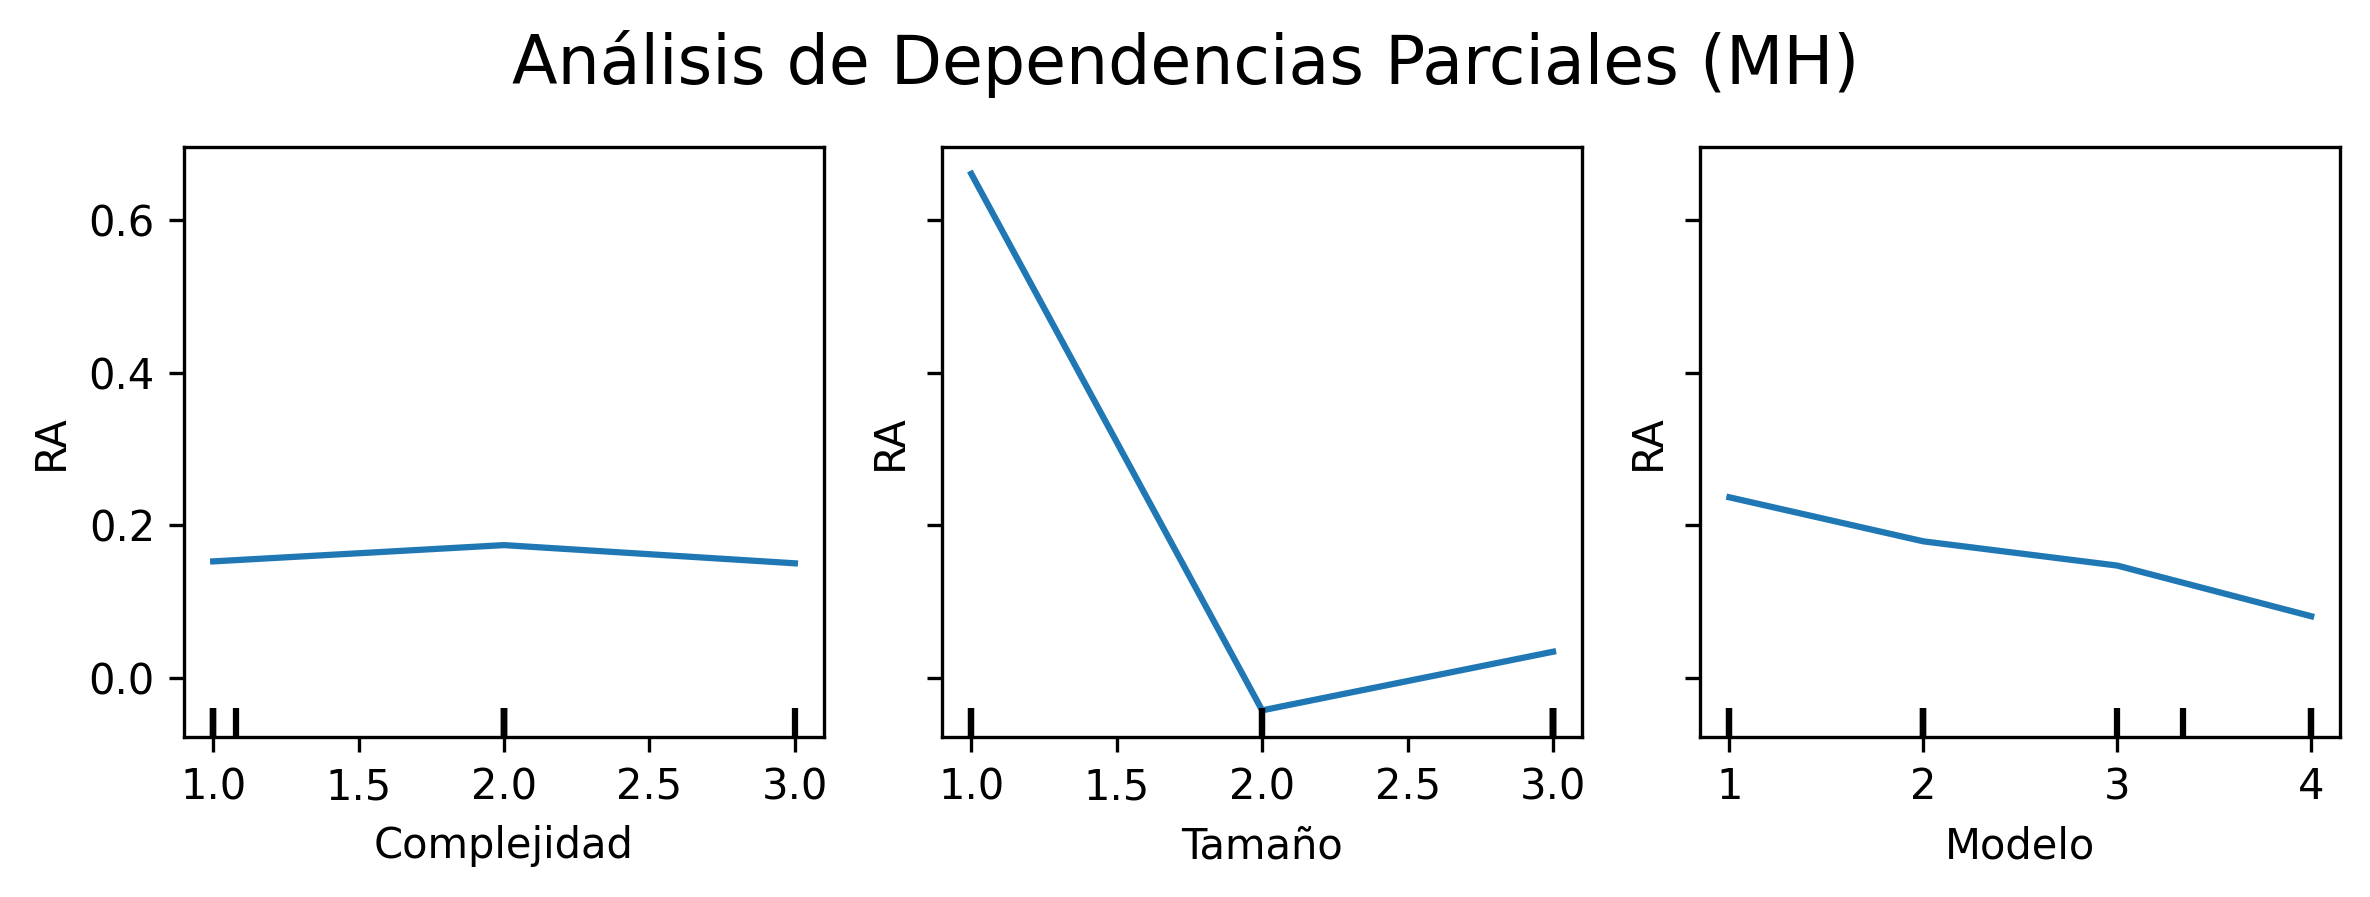
\includegraphics[width=1.0\linewidth]{Plantilla_TFG_latex//imagenes//Inf//Resultados/P1/pda_mh.png}
    \label{fig:pda_mh}}
    \hfill
    \subfloat{ 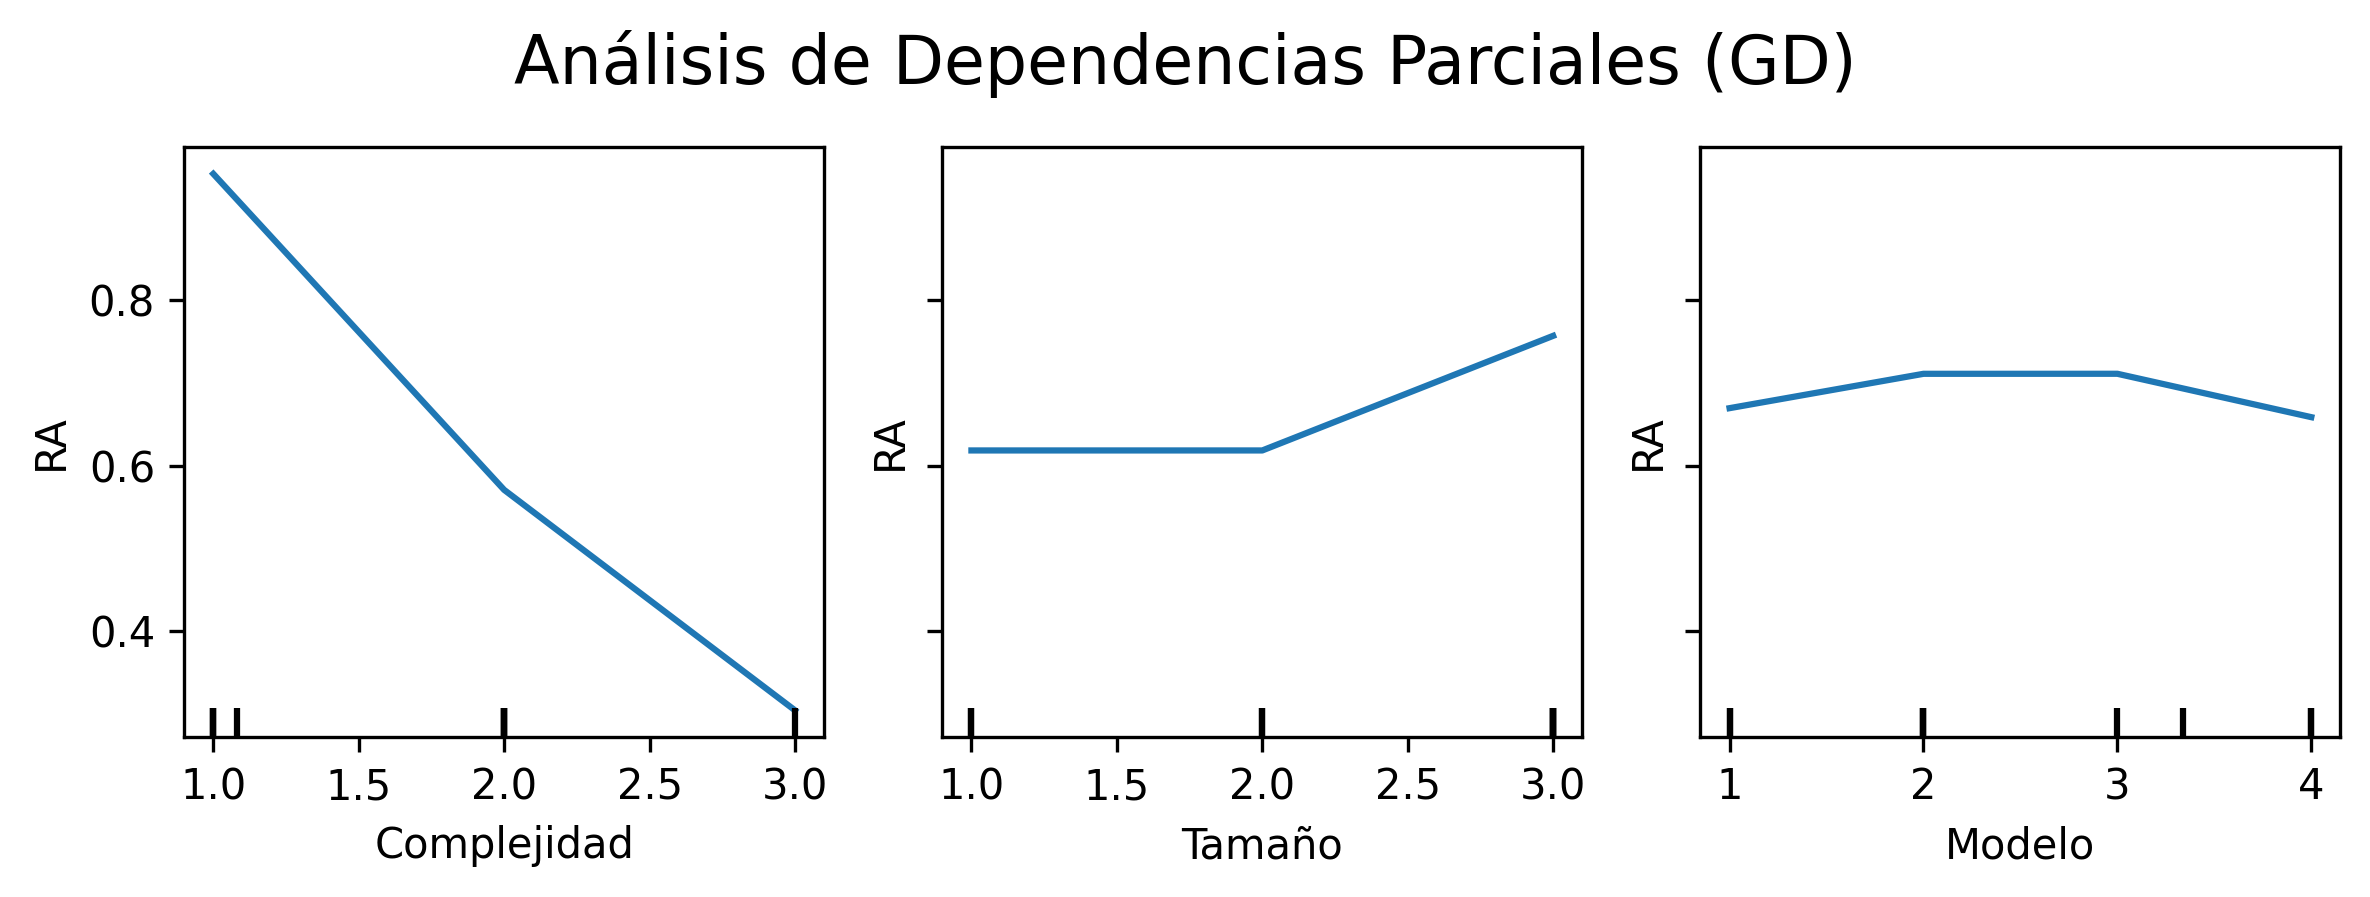
\includegraphics[width=1.0\linewidth]{Plantilla_TFG_latex//imagenes//Inf//Resultados/P1/pda_gd.png}    
    \label{fig:pda_gd}}   
    \caption[Análisis de dependencias parciales del rendimiento relativo al clasificador aleatorio en función de la complejidad del conjunto de datos, el tamaño del conjunto de datos y el número de parámetros del modelo]{Análisis de dependencias parciales del rendimiento relativo al clasificador aleatorio (RA) en función de la complejidad del conjunto de datos, el tamaño del conjunto de datos y el número de parámetros del modelo, para modelos entrenados con AdamW y RMSProp (GD); y SHADE y SHADE-ILS (MH). La primera fila de gráficos muestra los resultados obtenidos con MH, mientras que la segunda corresponde a GD. En cada conjunto de gráficos, el primer panel representa la relación entre la complejidad de la tarea y el RA, el segundo panel muestra el efecto del tamaño del conjunto de datos sobre el RA, y el tercero analiza la influencia del número de parámetros del modelo en el RA. Una tendencia decreciente indica un impacto negativo en el rendimiento, mientras que una tendencia creciente sugiere una mejora en el desempeño del modelo. Se observa que GD es más sensible a la complejidad de la tarea, mientras que MH muestra una caída abrupta en rendimiento con conjuntos de datos más grandes.}
    \label{fig:pda}
\end{figure}




\textbf{En el caso de las MH}, vemos que \textbf{las gráficas correspondientes al tamaño del modelo y la complejidad del conjunto de datos son prácticamente planas}, por lo que concluimos que \textbf{estos dos factores no afectan al rendimiento de los modelos entrenados con técnicas MH}. En contraposición, y contrariamente a la hipótesis planteada, la pendiente correspondiente a \textbf{la cantidad de ejemplos} en el conjunto de datos es muy acusada y negativa, lo que quiere decir que \textbf{este factor influye de manera inversamente proporcional al rendimiento de los modelos. Es decir, cuantos más datos de entrenamiento, peor rinde el modelo.}


\textbf{Con respecto al GD}, tenemos que \textbf{el número de ejemplos y el tamaño del modelo afectan en mucha menor medida que la complejidad de la tarea}. Aunque estos efectos son suaves, podemos observar ciertas tendencias que corroboran lo que conocemos a nivel teórico y verifica la hipótesis planteada. Generalmente, cuantos más ejemplos de entrenamiento tengamos mejor rendimiento tendremos, ya que al tener una muestra mayor los modelos pueden aprender más patrones y más complejos. Por otro lado, sabemos que aumentar el número de parámetros en un modelo no siempre equivale a un mejor rendimiento, y si lo aumentamos sin un criterio concreto podemos caer en un sobreajuste que empeore el rendimiento. Estas ideas pueden observarse de manera leve.

\textbf{Con la complejidad de la tarea sí que se observa una caída brusca de rendimiento conforme ésta crece}. De nuevo corroboramos la literatura y, además, podemos cuantificar y comparar. \textbf{En resumen, para optimizadores basados en GD el incremento de la complejidad de la tarea afecta muy negativamente al rendimiento del modelo}, mientras que el número de parámetros y el número de ejemplos afectan de manera leve, con unas interacciones que deben ser analizadas más minuciosamente. \textbf{En el caso de las MH, es el incremento del número de ejemplos el que contribuye a empeorar rápidamente el rendimiento de los modelos}, mientras que la complejidad del conjunto de datos y el número de parámetros del modelo no afectan prácticamente.






\subsubsection{Experimento 3: Análisis de los tiempos de ejecución en el entrenamiento con MH, tanto en MLPs como en ConvNets}

La hipótesis que planteamos ahora es que \textbf{el tiempo de ejecución de los algoritmos de entrenamiento varía significativamente entre las MH y el GD, siendo las primeras generalmente más costosas computacionalmente}. Específicamente, esperamos que SHADE-ILS tenga un mayor tiempo de ejecución en comparación con AdamW, debido a la naturaleza exploratoria de las metaheurísticas en el espacio de soluciones. Esperamos también que esta diferencia de tiempo tenga como base una ejecución menos optimizada, traducida en mayor tiempo de ejecución por época.

Con la intención de comprender mejor los tiempos de ejecución de ambas estrategias, vamos a comparar los tiempos de los algoritmos SHADE-ILS y AdamW, ya que son dos métodos utilizados en los dos experimentos anteriores y por tanto con los que venimos tratando. Como SHADE forma parte de la ejecución del algoritmo SHADE-ILS, analizaremos también el tiempo del primero a partir del segundo. Las tareas que hemos medido, aprovechando experimentos anteriores, junto con el tiempo de ejecución (en segundos), el número de instancias del conjunto y el número de parámetros del modelo, se pueden observar en la Tabla \ref{tab:tiempos}. En base a estas dos variables mostramos gráficamente el tiempo consumido en la Figura \ref{fig:tiemposgraf}.

\begin{table}[]
\resizebox{\textwidth}{!}{\begin{tabular}{|c|c|c|c|c|c|}
\hline
\textbf{Conjunto} & \textbf{Instancias} & \textbf{Modelo} & \textbf{Tamaño Modelo} & \textbf{SHADE-ILS} & \textbf{AdamW}   \\ \hline
BCW               & 569                 & MLP1            & 2238                   & \textbf{136.436}   & \textbf{2.442}   \\ \hline
BCW               & 569                 & MLP2            & 6462                   & \textbf{147.795}   & \textbf{2.448}   \\ \hline
BCW               & 569                 & MLP5            & 85000                  & \textbf{251.935}   & \textbf{2.611}   \\ \hline
BCW               & 569                 & MLP11           & 1400000                & \textbf{1791.067}  & \textbf{3.103}   \\ \hline
BHP               & 506                 & MLP1            & 2238                   & \textbf{56.217}    & \textbf{1.041}   \\ \hline
BHP               & 506                 & MLP2            & 6462                   & \textbf{61.645}    & \textbf{1.005}   \\ \hline
BHP               & 506                 & MLP5            & 85000                  & \textbf{110.071}   & \textbf{1.197}   \\ \hline
BHP               & 506                 & MLP11           & 1400000                & \textbf{833.789}   & \textbf{1.385}   \\ \hline
WQC               & 4898                & MLP1            & 2238                   & \textbf{800.998}   & \textbf{9.691}   \\ \hline
WQC               & 4898                & MLP2            & 6462                   & \textbf{867.628}   & \textbf{10.065}  \\ \hline
WQC               & 4898                & MLP5            & 85000                  & \textbf{1111.359}  & \textbf{12.283}  \\ \hline
WQC               & 4898                & MLP11           & 1400000                & \textbf{2395.200}  & \textbf{17.922}  \\ \hline
WQR               & 4898                & MLP1            & 2238                   & \textbf{785.936}   & \textbf{9.677}   \\ \hline
WQR               & 4898                & MLP2            & 6462                   & \textbf{856.806}   & \textbf{10.111}  \\ \hline
WQR               & 4898                & MLP5            & 85000                  & \textbf{1123.316}  & \textbf{11.907}  \\ \hline
WQR               & 4898                & MLP11           & 1400000                & \textbf{2054.672}  & \textbf{15.203}  \\ \hline
MNIST             & 15000               & LeNet5          & 62000                  & \textbf{7254.432}  & \textbf{54.999}  \\ \hline
MNIST             & 15000               & ResNet15        & 500000                 & \textbf{7991.074}  & \textbf{61.035}  \\ \hline
MNIST             & 15000               & ResNet57        & 1400000                & \textbf{8785.166}  & \textbf{72.317}  \\ \hline
FMNIST            & 15000               & LeNet5          & 62000                  & \textbf{6068.308}  & \textbf{56.922}  \\ \hline
FMNIST            & 15000               & ResNet15        & 500000                 & \textbf{6735.368}  & \textbf{63.989}  \\ \hline
FMNIST            & 15000               & ResNet57        & 1400000                & \textbf{10914.907} & \textbf{73.486}  \\ \hline
CIFAR             & 15000               & LeNet5          & 62000                  & \textbf{7453.761}  & \textbf{107.512} \\ \hline
CIFAR             & 15000               & ResNet15        & 500000                 & \textbf{8164.679}  & \textbf{113.781} \\ \hline
CIFAR             & 15000               & ResNet57        & 1400000                & \textbf{8812.613}  & \textbf{123.113} \\ \hline
\end{tabular}}
\caption[Comparación de tiempos entre los algoritmos SHADE-ILS y AdamW]{Tabla comparativa que muestra los tiempos de ejecución (en segundos) de los algoritmos SHADE-ILS y AdamW. Se muestra el conjunto de datos con el número de ejemplos correspondiente, además del modelo que se entrena con el número de parámetros que tiene. Se observa un incremento significativo en los tiempos de ejecución de SHADE-ILS con respecto a AdamW conforme aumenta la complejidad y el tamaño de los modelos y/o de los conjuntos de datos.}
\label{tab:tiempos}
\end{table}


\begin{figure}
    \centering
    \subfloat{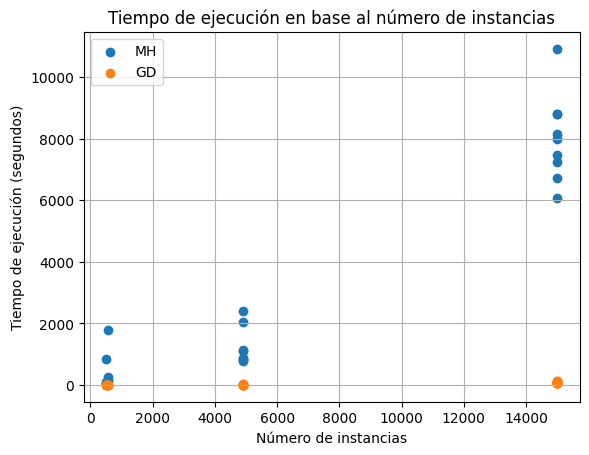
\includegraphics[width=0.85\linewidth]{Plantilla_TFG_latex//imagenes//Inf//Resultados/tiempo/instancias.png}\label{fig:tiempoinst}}
    \hfill
    \subfloat{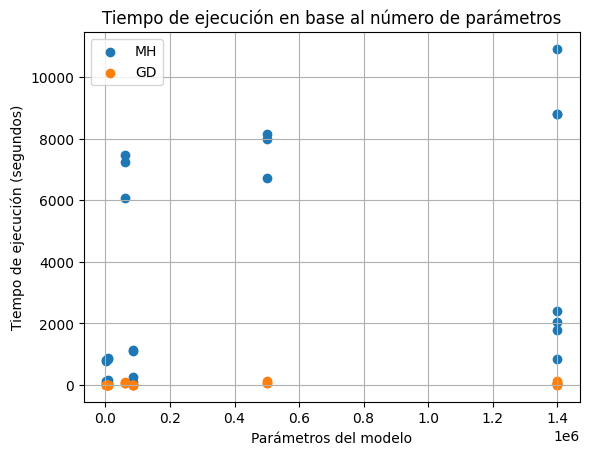
\includegraphics[width=0.85\linewidth]{Plantilla_TFG_latex//imagenes//Inf//Resultados/tiempo/parametros.png}\label{fig:tiempoparam}}
    \caption[Representación gráfica del tiempo de ejecución de los algoritmos SHADE-ILS y AdamW en función del número de parámetros del modelo]{Tiempo de ejecución (en segundos) de SHADE-ILS (MH) y AdamW (GD) en el entrenamiento en función del número de instancias del conjunto de datos (arriba) y del número de parámetros del modelo (abajo). Se observa que SHADE-ILS (azul) presenta tiempos de ejecución considerablemente mayores en comparación con AdamW (naranja), especialmente a medida que aumenta el número de instancias y la cantidad de parámetros del modelo. En particular, el tiempo de ejecución de SHADE-ILS crece de manera pronunciada con ambos factores, especialmente el número de instancias del conjunto de datos.}
    \label{fig:tiemposgraf}
\end{figure}


\begin{figure}
    \centering
    \subfloat{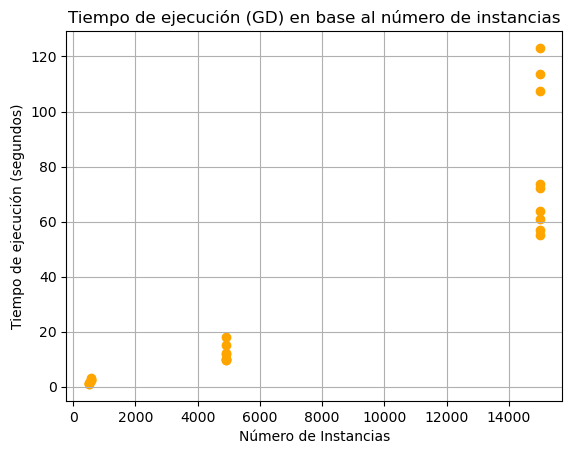
\includegraphics[width=0.85\linewidth]{Plantilla_TFG_latex//imagenes//Inf//Resultados/tiempo/instancias_gd.png}\label{fig:tiempoinst_gd}}
    \hfill
    \subfloat{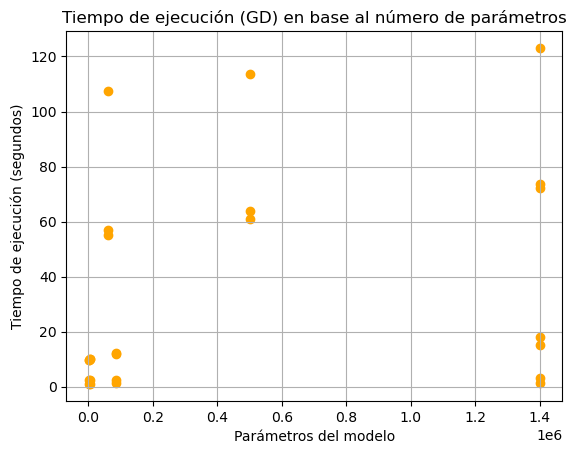
\includegraphics[width=0.85\linewidth]{Plantilla_TFG_latex//imagenes//Inf//Resultados/tiempo/parametros_gd.png}\label{fig:tiempoparam_gd}}
    \caption[Representación gráfica del tiempo de ejecución de AdamW en función del número de parámetros del modelo]{Tiempo de ejecución (en segundos) de AdamW (GD) en el entrenamiento en función del número de instancias del conjunto de datos (arriba) y del número de parámetros del modelo (abajo). Se observa que el número de instancias tiene un efecto mucho mayor que el número de parámetros del modelo.}
    \label{fig:tiemposgraf}
\end{figure}





  

Observando la Figura \ref{fig:tiempoparam}, vemos que la diferencia de tiempos entre algoritmos aumenta en menor medida que en la Figura \ref{fig:tiempoinst}. Además, en la Figura \ref{fig:tiempoparam} existe una amplitud muy grande entre la ejecución más rápida y más lenta del algoritmo SHADE-ILS, variabilidad que viene dada por las ejecuciones con distinto número de instancias, mientras que en la Figura \ref{fig:tiempoinst} los tiempos de las distintas ejecuciones son más compactos. Por tanto podemos afirmar que el número de instancias del conjunto de datos influye más en el tiempo de ejecución de las MH que el número de parámetros del modelo

Vemos clara la lentitud de la opción MH en comparación con la estrategia de GD, vamos pues a analizar de dónde surge esa diferencia y si es esperable a nivel teórico ya que asignamos más ejecuciones a los algoritmos MH. Elegiremos como referencia el caso de FMNIST con el modelo ResNet57. Mientras que SHADE-ILS tarda 10914.907 segundos, AdamW consume 73.486, es decir 148 veces más. Tenemos que tener en cuenta que asignamos más recursos computacionales a la ejecución de SHADE-ILS, pero la diferencia no se corresponde con la teoría. AdamW realiza 20 evaluaciones del conjunto de entrenamiento, mientras que SHADE-ILS hace 4200, 210 veces más. Por lo tanto mejoramos el tiempo que se supone que tendría a nivel teórico.

Observando las figuras \ref{fig:tiempoinst_gd} y\ref{fig:tiempoparam_gd} vemos que el número de ejemplos del conjunto de entrenamiento también tiene mayor peso en el tiempo de ejecución de AdamW, al igual que ocurría en el caso del algoritmo MH. El rango en el que se mueve el número de ejemplos (15 mil) es mucho menor del que se mueve el número de parámetros (1 millón aproximadamente), por lo que \textbf{este tiene un efecto proporcionalmente mucho mayor, del orden de 7 a 10 veces más.}


Vamos a desglosar los tiempos del algoritmo SHADE-ILS para comprenderlo mejor. La función de error propia que hemos implementado para las MH tarda 2.107 segundos en cada evaluación del conjunto de entrenamiento. Como SHADE-ILS ejecuta alrededor de 4200 evaluaciones de las cuales 4000 son realizadas con esa función, en total tenemos que consume 8428 segundos. Las otras 200 evaluaciones se llevan a cabo por el algoritmo de búsqueda local, que consume 4.158 segundos por eje por ejecución, lo que se traduce en un total de 831.600 segundos. Como a nivel abstracto ejecutamos 20 épocas (cada época son 200 evaluaciones de SHADE y 10 de búsqueda local), guardamos un histórico con 20 modelos a los que calculamos el error de validación y \textit{accuracy}, en lo que consumimos 66.400 segundos, que hacen un total de 9326.000 segundos. 

Esa diferencia de tiempo con los 10914.907 segundos totales son principalmente a las funciones de mutación y de cruce. Vamos a suponer que consumen el mismo tiempo y vamos a despreciar otras operaciones secundarias. Como SHADE ejecuta 4000 evaluaciones y tenemos 10 individuos, habrá 400 generaciones, lo que supone 8000 operaciones entre cruces y mutaciones. La diferencia entre el tiempo de la Tabla \ref{tab:tiempos} y el que hemos calculado en el párrafo anterior es de 1588.907 segundos, que si los atribuimos a las operaciones de cruce y mutación tenemos que consumen 0.199 segundos por operación. 

Concluimos por tanto, que \textbf{en términos de tiempo de ejecución por época las MH no son más lentas que el GD, de hecho lo mejoran. Sin embargo necesitan de muchas más ejecuciones para conseguir resultados que puedan asemejarse, en el mejor de los casos, a los obtenidos por optimizadores basados en GD}. Tenemos además un desglose de los tiempos que consumen las funciones que integran el algoritmo SHADE-ILS. La búsqueda local es la que más tiempo consume por ejecución, seguida de la operación de evaluar el conjunto de validación y obtener el valor de \textit{accuracy}, aunque precisamente estas dos últimas operaciones son las que menos se ejecutan. 

Como conclusión final del experimento, obtenemos dos afirmaciones:

\begin{enumerate}

\item El número de instancias del conjunto de datos con el que entrenamos influye más en el tiempo de entrenamiento que el número de parámetros del modelo, del orden de 7 a 10 veces más. Esto ocurre tanto para MH como para GD

\item En términos de tiempo de ejecución por época, las técnicas MH requieren menos tiempo de ejecución que los optimizadores basados en GD, resultado contrario a lo planteado en la hipótesis. Sin embargo, el hecho de que se necesiten muchas más épocas (del orden de 100 o 200 veces más) en las primeras para obtener resultados que se acerquen a las segundas, hace que el tiempo total de ejecución sea mucho mayor en las MH.

\end{enumerate}





%%%%%%%%%%%%%%%%%%%%%%%%%%%%%


\subsubsection{Experimento 4: Análisis comparativo de las propuestas propias} \label{sec:res_propias}



% Please add the following required packages to your document preamble:
% \usepackage{multirow}
\begin{table}[tbp]
\centering
\resizebox{\textwidth}{!}{\begin{tabular}{|c|c|ccc|ccc|}
\hline
\multirow{2}{*}{\textbf{Conjunto}} & \multirow{2}{*}{\textbf{Modelo}} & \multicolumn{3}{c|}{\textbf{SHADE}}                                                         & \multicolumn{3}{c|}{\textbf{SHADE-GD}}                                                                            \\ \cline{3-8} 
                                   &                                  & \multicolumn{1}{c|}{Train}          & \multicolumn{1}{c|}{Test}    & Métrica                & \multicolumn{1}{c|}{Train}            & \multicolumn{1}{c|}{Test}             & Métrica                           \\ \hline
\multirow{4}{*}{BCW}               & 1                                & \multicolumn{1}{c|}{0.112}          & \multicolumn{1}{c|}{0.187}   & \textbf{0.931}         & \multicolumn{1}{c|}{\textbf{0.108}}   & \multicolumn{1}{c|}{\textbf{0.181}}   & 0.915                             \\ \cline{2-8} 
                                   & 2                                & \multicolumn{1}{c|}{0.215}          & \multicolumn{1}{c|}{0.493}   & 0.725                  & \multicolumn{1}{c|}{\textbf{0.118}}   & \multicolumn{1}{c|}{\textbf{0.222}}   & \textbf{0.953}                    \\ \cline{2-8} 
                                   & 5                                & \multicolumn{1}{c|}{0.636}          & \multicolumn{1}{c|}{0.646}   & 0.825                  & \multicolumn{1}{c|}{\textbf{0.106}}   & \multicolumn{1}{c|}{\textbf{0.452}}   & \textbf{0.879}                    \\ \cline{2-8} 
                                   & 11                               & \multicolumn{1}{c|}{0.701}          & \multicolumn{1}{c|}{0.693}   & 0.500                  & \multicolumn{1}{c|}{\textbf{0.279}}   & \multicolumn{1}{c|}{\textbf{0.660}}   & \textbf{0.600}                    \\ \hline
\multirow{4}{*}{WQC}               & 1                                & \multicolumn{1}{c|}{2.100}          & \multicolumn{1}{c|}{2.475}   & \textbf{0.295}         & \multicolumn{1}{c|}{\textbf{1.082}}   & \multicolumn{1}{c|}{\textbf{1.304}}   & 0.171                             \\ \cline{2-8} 
                                   & 2                                & \multicolumn{1}{c|}{2.668}          & \multicolumn{1}{c|}{2.315}   & \textbf{0.214}         & \multicolumn{1}{c|}{\textbf{1.025}}   & \multicolumn{1}{c|}{\textbf{1.486}}   & 0.192                             \\ \cline{2-8} 
                                   & 5                                & \multicolumn{1}{c|}{2.303}          & \multicolumn{1}{c|}{2.304}   & 0.042                  & \multicolumn{1}{c|}{\textbf{0.953}}   & \multicolumn{1}{c|}{\textbf{1.495}}   & \textbf{0.203}                    \\ \cline{2-8} 
                                   & 11                               & \multicolumn{1}{c|}{2.662}          & \multicolumn{1}{c|}{2.302}   & 0.000                  & \multicolumn{1}{c|}{\textbf{1.104}}   & \multicolumn{1}{c|}{\textbf{3.982}}   & \textbf{0.211}                    \\ \hline
\multirow{4}{*}{BHP}               & 1                                & \multicolumn{1}{c|}{430.906}        & \multicolumn{1}{c|}{452.366} & $-1.922 \times 10^{4}$ & \multicolumn{1}{c|}{\textbf{13.977}}  & \multicolumn{1}{c|}{\textbf{33.099}}  & \textbf{0.650}                    \\ \cline{2-8} 
                                   & 2                                & \multicolumn{1}{c|}{430.970}        & \multicolumn{1}{c|}{428.226} & $-9.607 \times 10^{2}$ & \multicolumn{1}{c|}{\textbf{384.431}} & \multicolumn{1}{c|}{\textbf{128.808}} & \textbf{-4.610}                   \\ \cline{2-8} 
                                   & 5                                & \multicolumn{1}{c|}{429.719}        & \multicolumn{1}{c|}{435.000} & $-7.318 \times 10^{3}$ & \multicolumn{1}{c|}{\textbf{396.344}} & \multicolumn{1}{c|}{\textbf{324.056}} & \textbf{-0.932}                   \\ \cline{2-8} 
                                   & 11                               & \multicolumn{1}{c|}{469.788}        & \multicolumn{1}{c|}{454.786} & $-5.381 \times 10^{6}$ & \multicolumn{1}{c|}{\textbf{463.336}} & \multicolumn{1}{c|}{\textbf{453.891}} & \textbf{-1.294 $\times$ 10$^{5}$} \\ \hline
\multirow{4}{*}{WQR}               & 1                                & \multicolumn{1}{c|}{34.645}         & \multicolumn{1}{c|}{34.336}  & $-4.150 \times 10^{2}$ & \multicolumn{1}{c|}{\textbf{0.622}}   & \multicolumn{1}{c|}{\textbf{0.712}}   & \textbf{-2.624}                   \\ \cline{2-8} 
                                   & 2                                & \multicolumn{1}{c|}{35.425}         & \multicolumn{1}{c|}{30.956}  & $-2.020 \times 10^{3}$ & \multicolumn{1}{c|}{\textbf{0.562}}   & \multicolumn{1}{c|}{\textbf{1.548}}   & \textbf{-0.442}                   \\ \cline{2-8} 
                                   & 5                                & \multicolumn{1}{c|}{34.767}         & \multicolumn{1}{c|}{32.230}  & $-2.135 \times 10^{5}$ & \multicolumn{1}{c|}{\textbf{0.568}}   & \multicolumn{1}{c|}{\textbf{0.934}}   & \textbf{-3.447}                   \\ \cline{2-8} 
                                   & 11                               & \multicolumn{1}{c|}{\textbf{35.867}}         & \multicolumn{1}{c|}{32.176}  & $-1.951 \times 10^{6}$ & \multicolumn{1}{c|}{35.937}  & \multicolumn{1}{c|}{\textbf{32.039}}  & \textbf{-2.312 $\times$ 10$^{5}$} \\ \hline
\multirow{3}{*}{MNIST}             & LeNet5                           & \multicolumn{1}{c|}{2.424}          & \multicolumn{1}{c|}{2.277}   & 0.171                  & \multicolumn{1}{c|}{\textbf{0.110}}   & \multicolumn{1}{c|}{\textbf{1.930}}   & \textbf{0.529}                    \\ \cline{2-8} 
                                   & ResNet15                         & \multicolumn{1}{c|}{2.811}          & \multicolumn{1}{c|}{2.302}   & 0.100                  & \multicolumn{1}{c|}{\textbf{0.408}}   & \multicolumn{1}{c|}{2.301}            & 0.100                             \\ \cline{2-8} 
                                   & ResNet57                         & \multicolumn{1}{c|}{3.639}          & \multicolumn{1}{c|}{2.302}   & 0.082                  & \multicolumn{1}{c|}{\textbf{2.730}}   & \multicolumn{1}{c|}{2.302}            & \textbf{0.120}                    \\ \hline
\multirow{3}{*}{F-MNIST}           & LeNet5                           & \multicolumn{1}{c|}{1.498}          & \multicolumn{1}{c|}{2.291}   & 0.180                  & \multicolumn{1}{c|}{\textbf{0.705}}   & \multicolumn{1}{c|}{\textbf{2.140}}   & \textbf{0.360}                    \\ \cline{2-8} 
                                   & ResNet15                         & \multicolumn{1}{c|}{\textbf{2.668}} & \multicolumn{1}{c|}{2.303}   & 0.104                  & \multicolumn{1}{c|}{3.547}            & \multicolumn{1}{c|}{2.302}            & 0.100                             \\ \cline{2-8} 
                                   & ResNet57                         & \multicolumn{1}{c|}{2.525}          & \multicolumn{1}{c|}{2.303}   & 0.100                  & \multicolumn{1}{c|}{\textbf{1.389}}   & \multicolumn{1}{c|}{2.303}            & 0.100                             \\ \hline
\multirow{3}{*}{CIFAR-10G}        & LeNet5                           & \multicolumn{1}{c|}{2.548}          & \multicolumn{1}{c|}{2.300}   & 0.102                  & \multicolumn{1}{c|}{\textbf{1.483}}   & \multicolumn{1}{c|}{\textbf{2.275}}   & \textbf{0.142}                    \\ \cline{2-8} 
                                   & ResNet15                         & \multicolumn{1}{c|}{\textbf{2.536}} & \multicolumn{1}{c|}{2.303}   & \textbf{0.111}         & \multicolumn{1}{c|}{2.798}            & \multicolumn{1}{c|}{2.303}            & 0.096                             \\ \cline{2-8} 
                                   & ResNet57                         & \multicolumn{1}{c|}{2.723}          & \multicolumn{1}{c|}{2.303}   & 0.099                  & \multicolumn{1}{c|}{\textbf{2.701}}   & \multicolumn{1}{c|}{2.303}            & 0.093                             \\ \hline
\end{tabular}}
\caption[Comparación del desempeño de SHADE y SHADE-GD en el entrenamiento de modelos de aprendizaje profundo sobre conjuntos de datos tabulares e imágenes]{Comparación del desempeño de SHADE y SHADE-GD en el entrenamiento de modelos de aprendizaje profundo sobre conjuntos de datos tabulares e imágenes. Se presentan los errores de entrenamiento (\textit{Train}) y evaluación (\textit{Test}), junto con la métrica de desempeño utilizada en cada caso (\textbf{\textit{Balanced Accuracy}} para BCW y WQC, \textbf{\emph{R$^2$}}  para BHP y WQR, y \textbf{\textit{accuracy}} para MNIST, Fashion-MNIST y CIFAR-10 en escala de grises). Para datos tabulares, se emplean modelos MLP con distintas profundidades, mientras que para imágenes se evalúan modelos de la familia ConvNet (LeNet5, ResNet15 y ResNet57)  (columna Modelo). Los valores resaltados indican el mejor desempeño en cada caso. En las filas sin valores resaltados, ambos métodos presentan un rendimiento equivalente. Consideramos que el modelo con mejor rendimiento es el que tiene mejor valor en su métrica. Se observa que SHADE-GD generalmente supera a SHADE, especialmente en modelos más profundos y en conjuntos de datos tabulares, donde SHADE tiende a deteriorarse.}
\label{tab:shadevsshadegd}
\end{table}






\vspace{0.4cm}
\paragraph{SHADE y SHADE-GD\\}  


\mbox{}
\vspace{0.1cm}

Comentamos los resultados obtenidos del entrenamiento y que se muestran en la Tabla \ref{tab:shadevsshadegd}. SHADE-GD supera a SHADE en la mayoría de los escenarios, logrando menores errores en entrenamiento y prueba. La incorporación del descenso de gradiente mejora la optimización de los pesos, reduciendo el sobreajuste y favoreciendo la generalización. En contraste, SHADE muestra inconsistencias a medida que aumenta la complejidad del modelo, con errores significativamente mayores en entornos de alta dimensionalidad.

SHADE sufre mayor deterioro en la generalización, especialmente en modelos profundos y conjuntos de datos grandes como MNIST y CIFAR-10G, donde sus métricas de desempeño son muy bajas. SHADE-GD, en cambio, reduce la pérdida en entrenamiento sin aumentar drásticamente la pérdida en prueba, evitando estancamientos en soluciones subóptimas.

SHADE muestra un deterioro progresivo en arquitecturas con mayor número de parámetros, con un rendimiento deficiente en modelos MLP con 5 y 11 capas ocultas, así como en redes convolucionales complejas como ResNet15 y ResNet57. SHADE-GD mantiene un desempeño más estable y presenta mejoras en redes convolucionales, aunque persisten dificultades en modelos profundos.

\textbf{En clasificación, SHADE-GD obtiene mejores métricas, especialmente en modelos simples} como LeNet5, aunque sigue sin igualar métodos basados en gradientes en modelos más complejos. En regresión, SHADE muestra valores extremadamente negativos en $R^2$, mientras que SHADE-GD logra métricas más aceptables, destacando su ventaja en la minimización del error.

SHADE-GD sigue sin ser competitivo en redes profundas aplicadas a conjuntos de datos complejos como CIFAR-10G, posiblemente debido a una exploración inicial ineficiente en SHADE. Además, SHADE tiende a estancarse en soluciones subóptimas cuando la dimensionalidad del espacio de búsqueda es alta, resultando en métricas de evaluación deficientes.

\textbf{Como conclusión, SHADE-GD supera a SHADE en la mayoría de los casos, mostrando menor error y mejor desempeño, aunque aún enfrenta limitaciones en redes profundas y conjuntos de datos grandes}. Se requieren estrategias adicionales de optimización para mejorar su eficacia en escenarios más complejos.




% Please add the following required packages to your document preamble:
% \usepackage{multirow}
\begin{table}[tbp]
\resizebox{\textwidth}{!}{\begin{tabular}{|c|c|ccc|ccc|}
\hline
\multirow{2}{*}{\textbf{Conjunto}} & \multirow{2}{*}{\textbf{Modelo}} & \multicolumn{3}{c|}{\textbf{SHADE-ILS}}                                                            & \multicolumn{3}{c|}{\textbf{SHADE-ILS-GD}}                                                                    \\ \cline{3-8} 
                                   &                                  & \multicolumn{1}{c|}{Train}          & \multicolumn{1}{c|}{Test}           & Métrica                & \multicolumn{1}{c|}{Train}           & \multicolumn{1}{c|}{Test}            & Métrica                         \\ \hline
\multirow{4}{*}{BCW}               & 1                                & \multicolumn{1}{c|}{0.073}          & \multicolumn{1}{c|}{\textbf{0.142}} & \textbf{0.970}         & \multicolumn{1}{c|}{\textbf{0.062}}  & \multicolumn{1}{c|}{0.159}           & 0.941                           \\ \cline{2-8} 
                                   & 2                                & \multicolumn{1}{c|}{0.063}          & \multicolumn{1}{c|}{0.350}          & 0.932                  & \multicolumn{1}{c|}{0.063}           & \multicolumn{1}{c|}{0.350}           & 0.932                           \\ \cline{2-8} 
                                   & 5                                & \multicolumn{1}{c|}{0.055}          & \multicolumn{1}{c|}{\textbf{0.475}} & \textbf{0.891}         & \multicolumn{1}{c|}{\textbf{0.031}}  & \multicolumn{1}{c|}{0.616}           & 0.600                           \\ \cline{2-8} 
                                   & 11                               & \multicolumn{1}{c|}{\textbf{0.099}} & \multicolumn{1}{c|}{\textbf{0.491}} & \textbf{0.903}         & \multicolumn{1}{c|}{0.112}           & \multicolumn{1}{c|}{0.704}           & 0.500                           \\ \hline
\multirow{4}{*}{WQC}               & 1                                & \multicolumn{1}{c|}{1.098}          & \multicolumn{1}{c|}{1.235}          & 0.201                  & \multicolumn{1}{c|}{\textbf{1.068}}  & \multicolumn{1}{c|}{\textbf{1.224}}  & \textbf{0.226}                  \\ \cline{2-8} 
                                   & 2                                & \multicolumn{1}{c|}{1.078}          & \multicolumn{1}{c|}{1.340}          & 0.167                  & \multicolumn{1}{c|}{\textbf{1.065}}  & \multicolumn{1}{c|}{\textbf{1.400}}  & \textbf{0.306}                  \\ \cline{2-8} 
                                   & 5                                & \multicolumn{1}{c|}{0.963}          & \multicolumn{1}{c|}{1.405}          & 0.167                  & \multicolumn{1}{c|}{\textbf{0.951}}  & \multicolumn{1}{c|}{\textbf{1.328}}  & 0.166                           \\ \cline{2-8} 
                                   & 11                               & \multicolumn{1}{c|}{1.138}          & \multicolumn{1}{c|}{1.509}          & 0.167                  & \multicolumn{1}{c|}{\textbf{1.099}}  & \multicolumn{1}{c|}{\textbf{1.496}}  & 0.167                           \\ \hline
\multirow{4}{*}{BHP}               & 1                                & \multicolumn{1}{c|}{10.048}         & \multicolumn{1}{c|}{7.549}          & 0.576                  & \multicolumn{1}{c|}{\textbf{8.928}}  & \multicolumn{1}{c|}{\textbf{3.895}}  & \textbf{0.849}                  \\ \cline{2-8} 
                                   & 2                                & \multicolumn{1}{c|}{9.561}          & \multicolumn{1}{c|}{4.649}          & 0.747                  & \multicolumn{1}{c|}{9.561}           & \multicolumn{1}{c|}{4.649}           & 0.747                           \\ \cline{2-8} 
                                   & 5                                & \multicolumn{1}{c|}{13.594}         & \multicolumn{1}{c|}{14.556}         & -0.187                 & \multicolumn{1}{c|}{\textbf{11.689}} & \multicolumn{1}{c|}{\textbf{14.368}} & \textbf{-0.078}                 \\ \cline{2-8} 
                                   & 11                               & \multicolumn{1}{c|}{43.184}         & \multicolumn{1}{c|}{26.794}         & -97.405                & \multicolumn{1}{c|}{43.184}          & \multicolumn{1}{c|}{26.794}          & -97.405                         \\ \hline
\multirow{4}{*}{WQR}               & 1                                & \multicolumn{1}{c|}{0.611}          & \multicolumn{1}{c|}{0.970}          & -1.987                 & \multicolumn{1}{c|}{\textbf{0.599}}  & \multicolumn{1}{c|}{\textbf{0.912}}  & \textbf{-1.898}                 \\ \cline{2-8} 
                                   & 2                                & \multicolumn{1}{c|}{0.579}          & \multicolumn{1}{c|}{0.826}          & -2.491                 & \multicolumn{1}{c|}{\textbf{0.521}}  & \multicolumn{1}{c|}{\textbf{0.620}}  & \textbf{-4.105}                 \\ \cline{2-8} 
                                   & 5                                & \multicolumn{1}{c|}{0.589}          & \multicolumn{1}{c|}{\textbf{0.724}} & -9.832 $\times$ 10$^2$ & \multicolumn{1}{c|}{\textbf{0.579}}  & \multicolumn{1}{c|}{0.747}           & \textbf{-2.347 $\times$ 10$^2$} \\ \cline{2-8} 
                                   & 11                               & \multicolumn{1}{c|}{0.601}          & \multicolumn{1}{c|}{\textbf{0.734}} & -7.953 $\times$ 10$^4$ & \multicolumn{1}{c|}{0.601}           & \multicolumn{1}{c|}{0.774}           & -7.953 $\times$ 10$^{4}$        \\ \hline
\multirow{3}{*}{MNIST}             & LeNet5                           & \multicolumn{1}{c|}{2.530}          & \multicolumn{1}{c|}{2.300}          & 0.066                  & \multicolumn{1}{c|}{2.530}           & \multicolumn{1}{c|}{2.300}           & 0.066                           \\ \cline{2-8} 
                                   & ResNet15                         & \multicolumn{1}{c|}{0.001}          & \multicolumn{1}{c|}{2.294}          & \textbf{0.115}         & \multicolumn{1}{c|}{0.001}           & \multicolumn{1}{c|}{2.292}           & 0.100                           \\ \cline{2-8} 
                                   & ResNet57                         & \multicolumn{1}{c|}{2.308}          & \multicolumn{1}{c|}{2.303}          & 0.100                  & \multicolumn{1}{c|}{\textbf{0.001}}  & \multicolumn{1}{c|}{2.303}           & 0.100                           \\ \hline
\multirow{3}{*}{F-MNIST}           & LeNet5                           & \multicolumn{1}{c|}{0.403}          & \multicolumn{1}{c|}{1.807}          & 0.366                  & \multicolumn{1}{c|}{\textbf{0.327}}  & \multicolumn{1}{c|}{\textbf{1.646}}  & \textbf{0.462}                  \\ \cline{2-8} 
                                   & ResNet15                         & \multicolumn{1}{c|}{3.547}          & \multicolumn{1}{c|}{2.302}          & \textbf{0.100}         & \multicolumn{1}{c|}{\textbf{0.349}}  & \multicolumn{1}{c|}{2.302}           & 0.063                           \\ \cline{2-8} 
                                   & ResNet57                         & \multicolumn{1}{c|}{2.673}          & \multicolumn{1}{c|}{2.303}          & 0.100                  & \multicolumn{1}{c|}{\textbf{1.208}}  & \multicolumn{1}{c|}{2.303}           & 0.100                           \\ \hline
\multirow{3}{*}{CIFAR-10G}        & LeNet5                           & \multicolumn{1}{c|}{2.568}          & \multicolumn{1}{c|}{2.301}          & 0.114                  & \multicolumn{1}{c|}{2.568}           & \multicolumn{1}{c|}{2.301}           & 0.114                           \\ \cline{2-8} 
                                   & ResNet15                         & \multicolumn{1}{c|}{\textbf{1.697}} & \multicolumn{1}{c|}{2.303}          & \textbf{0.103}         & \multicolumn{1}{c|}{3.504}           & \multicolumn{1}{c|}{2.303}           & 0.093                           \\ \cline{2-8} 
                                   & ResNet57                         & \multicolumn{1}{c|}{2.579}          & \multicolumn{1}{c|}{2.303}          & \textbf{0.100}         & \multicolumn{1}{c|}{\textbf{2.415}}  & \multicolumn{1}{c|}{2.303}           & 0.096                           \\ \hline
\end{tabular}}
\caption[Comparación del desempeño de SHADE-ILS y SHADE-ILS-GD en el entrenamiento de modelos de aprendizaje profundo sobre conjuntos de datos tabulares e imágenes]{Comparación del desempeño de SHADE-ILS y SHADE-ILS-GD en el entrenamiento de modelos de aprendizaje profundo sobre conjuntos de datos tabulares e imágenes. Se presentan los errores de entrenamiento (\textit{Train}) y evaluación (\textit{Test}), junto con la métrica de desempeño utilizada en cada caso (\textit{Balanced Accuracy} para BCW y WQC, $R^2$  para BHP y WQR, y \textit{accuracy} para MNIST, Fashion-MNIST y CIFAR-10 en escala de grises). Para datos tabulares, se emplean modelos MLP con distintas profundidades, mientras que para imágenes se evalúan modelos de la familia ConvNet (LeNet5, ResNet15 y ResNet57)  (columna Modelo). Los valores resaltados indican el mejor desempeño en cada caso. En las filas sin valores resaltados, ambos métodos presentan un rendimiento equivalente. Consideramos que el modelo con mejor rendimiento es el que tiene mejor valor en su métrica. No hay una diferencia clara entre ambos optimizadores, aunque se observa que SHADE-ILS en su versión original consigue más robustez, siendo más estable en la mayoría de tareas.}
\label{tab:ilsvsilsgd}
\end{table}

\vspace{0.4cm}
\paragraph{SHADE-ILS y SHADE-ILS-GD\\} 

\mbox{}
\vspace{0.1cm}


Comentamos los resultados obtenidos del entrenamiento y que se muestran en la Tabla \ref{tab:ilsvsilsgd}. El rendimiento de SHADE-ILS y SHADE-ILS-GD varía según la complejidad del problema y la arquitectura de la red utilizada. Aunque SHADE-ILS-GD puede reducir el error en algunos casos, no siempre mejora la capacidad de generalización del modelo. En redes profundas y conjuntos de datos de mayortamaño,\textbf{ la combinación con GD no siempre aporta ventajas significativas sobre SHADE-ILS}.

\textbf{SHADE-ILS muestra mayor estabilidad en modelos profundos}, donde la introducción de GD en SHADE-ILS-GD a menudo induce fluctuaciones en la convergencia. En particular, en la tarea de clasificación sobre un conjunto de datos con alta dimensionalidad, SHADE-ILS-GD presentó variaciones bruscas en el valor de la métrica entre iteraciones, mientras que SHADE-ILS mantuvo una convergencia más uniforme. En tareas de regresión tabular, SHADE-ILS-GD mostró mejoras esporádicas en el coeficiente $R^2$, pero también una mayor propensión al sobreajuste cuando se aumentó la cantidad de capas en la red.

\textbf{En problemas de regresión, SHADE-ILS-GD mejora la generalización en redes poco profundas}, como en el caso de un modelo de tres capas donde redujo el error de evaluación en un 7\% (Tabla \ref{tab:ilsvsilsgd}). Sin embargo, \textbf{en redes más complejas, esta ventaja desaparece}, e incluso el modelo entrenado con SHADE-ILS mantiene un desempeño más estable en el conjunto de entrenamiento. En clasificación, SHADE-ILS-GD no muestra mejoras consistentes y, en algunos casos, como en MNIST, obtuvo un valor de \textit{accuracy} 3\% inferior a la de SHADE-ILS. En modelos convolucionales aplicados a conjuntos de datos de imágenes, SHADE-ILS-GD rara vez aporta mejoras y, en ocasiones, introduce sobreajuste, como se evidenció en una prueba donde el error de entrenamiento disminuyó sin que la métrica en el conjunto de prueba mejorara.

\textbf{Como conclusión, SHADE-ILS es una opción más eficiente y estable en redes profundas, mientras que SHADE-ILS-GD puede aportar mejoras en regresión con arquitecturas simples}. Sin embargo, el refinamiento con GD no garantiza una mejor generalización y puede inducir sobreajuste o aumentar significativamente el tiempo de cómputo sin beneficios claros. En datos tabulares, SHADE-ILS-GD presenta mejoras ocasionales, pero en imágenes y redes profundas, SHADE-ILS sigue siendo la alternativa más confiable. Estos resultados sugieren que la incorporación de GD en SHADE-ILS debe evaluarse caso por caso, ya que sus beneficios no son universales y dependen del tipo de tarea y arquitectura utilizada.



% Please add the following required packages to your document preamble:
% \usepackage{multirow}
\begin{table}[tbp]
\resizebox{\textwidth}{!}{\begin{tabular}{|c|c|ccc|ccc|}
\hline
\multirow{2}{*}{\textbf{Conjunto}} & \multirow{2}{*}{\textbf{Modelo}} & \multicolumn{3}{c|}{\textbf{SHADE-GD}}                                                               & \multicolumn{3}{c|}{\textbf{SHADE-ILS-GD}}                                                                      \\ \cline{3-8} 
                                   &                                  & \multicolumn{1}{c|}{Train}          & \multicolumn{1}{c|}{Test}           & Métrica                  & \multicolumn{1}{c|}{Train}           & \multicolumn{1}{c|}{Test}            & Métrica                           \\ \hline
\multirow{4}{*}{BCW}               & 1                                & \multicolumn{1}{c|}{0.108}          & \multicolumn{1}{c|}{0.181}          & 0.915                    & \multicolumn{1}{c|}{\textbf{0.062}}  & \multicolumn{1}{c|}{\textbf{0.159}}  & \textbf{0.941}                    \\ \cline{2-8} 
                                   & 2                                & \multicolumn{1}{c|}{0.118}          & \multicolumn{1}{c|}{\textbf{0.222}} & \textbf{0.953}           & \multicolumn{1}{c|}{\textbf{0.063}}  & \multicolumn{1}{c|}{0.350}           & 0.932                             \\ \cline{2-8} 
                                   & 5                                & \multicolumn{1}{c|}{0.106}          & \multicolumn{1}{c|}{\textbf{0.452}} & \textbf{0.879}           & \multicolumn{1}{c|}{\textbf{0.031}}  & \multicolumn{1}{c|}{0.616}           & 0.600                             \\ \cline{2-8} 
                                   & 11                               & \multicolumn{1}{c|}{0.279}          & \multicolumn{1}{c|}{\textbf{0.660}} & \textbf{0.600}           & \multicolumn{1}{c|}{\textbf{0.112}}  & \multicolumn{1}{c|}{0.704}           & 0.500                             \\ \hline
\multirow{4}{*}{WQC}               & 1                                & \multicolumn{1}{c|}{1.082}          & \multicolumn{1}{c|}{1.304}          & 0.171                    & \multicolumn{1}{c|}{\textbf{1.068}}  & \multicolumn{1}{c|}{\textbf{1.224}}  & \textbf{0.226}                    \\ \cline{2-8} 
                                   & 2                                & \multicolumn{1}{c|}{\textbf{1.025}} & \multicolumn{1}{c|}{1.486}          & 0.192                    & \multicolumn{1}{c|}{1.065}           & \multicolumn{1}{c|}{\textbf{1.400}}  & \textbf{0.306}                    \\ \cline{2-8} 
                                   & 5                                & \multicolumn{1}{c|}{0.953}          & \multicolumn{1}{c|}{1.495}          & \textbf{0.203}           & \multicolumn{1}{c|}{0.951}           & \multicolumn{1}{c|}{\textbf{1.328}}  & 0.166                             \\ \cline{2-8} 
                                   & 11                               & \multicolumn{1}{c|}{1.104}          & \multicolumn{1}{c|}{3.982}          & \textbf{0.211}           & \multicolumn{1}{c|}{\textbf{1.099}}  & \multicolumn{1}{c|}{\textbf{1.496}}  & 0.167                             \\ \hline
\multirow{4}{*}{BHP}               & 1                                & \multicolumn{1}{c|}{13.977}         & \multicolumn{1}{c|}{33.099}         & 0.650                    & \multicolumn{1}{c|}{\textbf{8.928}}  & \multicolumn{1}{c|}{\textbf{3.895}}  & \textbf{0.849}                    \\ \cline{2-8} 
                                   & 2                                & \multicolumn{1}{c|}{384.431}        & \multicolumn{1}{c|}{128.808}        & -4.610                   & \multicolumn{1}{c|}{\textbf{9.561}}  & \multicolumn{1}{c|}{\textbf{4.649}}  & \textbf{0.747}                    \\ \cline{2-8} 
                                   & 5                                & \multicolumn{1}{c|}{396.344}        & \multicolumn{1}{c|}{324.056}        & -0.932                   & \multicolumn{1}{c|}{\textbf{11.689}} & \multicolumn{1}{c|}{\textbf{14.368}} & \textbf{-0.078}                   \\ \cline{2-8} 
                                   & 11                               & \multicolumn{1}{c|}{463.336}        & \multicolumn{1}{c|}{453.891}        & -1.294 $\times$ 10$^{5}$ & \multicolumn{1}{c|}{\textbf{43.184}} & \multicolumn{1}{c|}{\textbf{26.794}} & \textbf{-97.405}                  \\ \hline
\multirow{4}{*}{WQR}               & 1                                & \multicolumn{1}{c|}{0.622}          & \multicolumn{1}{c|}{\textbf{0.712}} & -2.624                   & \multicolumn{1}{c|}{\textbf{0.599}}  & \multicolumn{1}{c|}{0.912}           & \textbf{-1.898}                   \\ \cline{2-8} 
                                   & 2                                & \multicolumn{1}{c|}{0.562}          & \multicolumn{1}{c|}{1.548}          & \textbf{-0.442}          & \multicolumn{1}{c|}{\textbf{0.521}}  & \multicolumn{1}{c|}{\textbf{0.620}}  & -4.105                            \\ \cline{2-8} 
                                   & 5                                & \multicolumn{1}{c|}{\textbf{0.568}} & \multicolumn{1}{c|}{0.934}          & \textbf{-3.447}          & \multicolumn{1}{c|}{0.579}           & \multicolumn{1}{c|}{\textbf{0.747}}  & -2.347 $\times$ 10$^2$            \\ \cline{2-8} 
                                   & 11                               & \multicolumn{1}{c|}{35.937}         & \multicolumn{1}{c|}{32.039}         & -2.312 $\times$ 10$^{5}$ & \multicolumn{1}{c|}{\textbf{0.601}}  & \multicolumn{1}{c|}{\textbf{0.774}}  & \textbf{-7.953 $\times$ 10$^{4}$} \\ \hline
\multirow{3}{*}{MNIST}             & LeNet5                           & \multicolumn{1}{c|}{\textbf{0.110}} & \multicolumn{1}{c|}{\textbf{1.930}} & \textbf{0.529}           & \multicolumn{1}{c|}{2.530}           & \multicolumn{1}{c|}{2.300}           & 0.066                             \\ \cline{2-8} 
                                   & ResNet15                         & \multicolumn{1}{c|}{0.408}          & \multicolumn{1}{c|}{\textbf{2.301}} & 0.100                    & \multicolumn{1}{c|}{\textbf{0.001}}  & \multicolumn{1}{c|}{2.292}           & 0.100                             \\ \cline{2-8} 
                                   & ResNet57                         & \multicolumn{1}{c|}{2.730}          & \multicolumn{1}{c|}{2.302}          & \textbf{0.120}           & \multicolumn{1}{c|}{\textbf{0.001}}  & \multicolumn{1}{c|}{2.303}           & 0.100                             \\ \hline
\multirow{3}{*}{F-MNIST}           & LeNet5                           & \multicolumn{1}{c|}{0.705}          & \multicolumn{1}{c|}{2.140}          & 0.360                    & \multicolumn{1}{c|}{\textbf{0.327}}  & \multicolumn{1}{c|}{\textbf{1.646}}  & \textbf{0.462}                    \\ \cline{2-8} 
                                   & ResNet15                         & \multicolumn{1}{c|}{3.547}          & \multicolumn{1}{c|}{2.302}          & \textbf{0.100}           & \multicolumn{1}{c|}{\textbf{0.349}}  & \multicolumn{1}{c|}{2.302}           & 0.063                             \\ \cline{2-8} 
                                   & ResNet57                         & \multicolumn{1}{c|}{1.389}          & \multicolumn{1}{c|}{2.303}          & 0.100                    & \multicolumn{1}{c|}{\textbf{1.208}}  & \multicolumn{1}{c|}{2.303}           & 0.100                             \\ \hline
\multirow{3}{*}{CIFAR-10G}        & LeNet5                           & \multicolumn{1}{c|}{\textbf{1.483}} & \multicolumn{1}{c|}{\textbf{2.275}} & \textbf{0.142}           & \multicolumn{1}{c|}{2.568}           & \multicolumn{1}{c|}{2.301}           & 0.114                             \\ \cline{2-8} 
                                   & ResNet15                         & \multicolumn{1}{c|}{\textbf{2.798}} & \multicolumn{1}{c|}{2.303}          & 0.096                    & \multicolumn{1}{c|}{3.504}           & \multicolumn{1}{c|}{2.303}           & 0.093                             \\ \cline{2-8} 
                                   & ResNet57                         & \multicolumn{1}{c|}{2.701}          & \multicolumn{1}{c|}{2.303}          & 0.093                    & \multicolumn{1}{c|}{\textbf{2.415}}  & \multicolumn{1}{c|}{2.303}           & 0.096                             \\ \hline
\end{tabular}}
\caption[Comparación del desempeño de SHADE-GD y SHADE-ILS-GD en el entrenamiento de modelos de aprendizaje profundo sobre conjuntos de datos tabulares e imágenes]{Comparación del desempeño de SHADE-ILS y SHADE-ILS-GD en el entrenamiento de modelos de aprendizaje profundo sobre conjuntos de datos tabulares e imágenes. Se presentan los errores de entrenamiento (\textit{Train}) y evaluación (\textit{Test}), junto con la métrica de desempeño utilizada en cada caso (\textit{Balanced Accuracy} para BCW y WQC, $R^2$  para BHP y WQR, y \textit{accuracy} para MNIST, Fashion-MNIST y CIFAR-10 en escala de grises). Para datos tabulares, se emplean modelos MLP con distintas profundidades, mientras que para imágenes se evalúan modelos de la familia ConvNet (LeNet5, ResNet15 y ResNet57)  (columna Modelo). Los valores resaltados indican el mejor desempeño en cada caso. En las filas sin valores resaltados, ambos métodos presentan un rendimiento equivalente. Consideramos que el modelo con mejor rendimiento es el que tiene mejor valor en su métrica. Aunque no hay una diferencia clara entre los dos optimizadores, existe un patrón reconocible, en el que se evidencia que SHADE-GD tiende a generalizar mejor mientras que SHADE-ILS-GD minimiza más la función de pérdida.}
\label{tab:shadegdvsilsgd}
\end{table}

\vspace{0.4cm}
\paragraph{SHADE-GD y SHADE-ILS-GD\\} 

\mbox{}
\vspace{0.1cm}

\textbf{En términos generales, SHADE-ILS-GD muestra un mejor rendimiento en los conjuntos de datos más complejos o con mayor variabilidad}. En particular, destaca en el conjunto BHP, donde logra mejoras sustanciales en las métricas de evaluación. Por ejemplo, en el modelo MLP1, el error en el conjunto de prueba se reduce drásticamente de 33.099 con SHADE-GD a 3.895 con SHADE-ILS-GD, lo que se traduce en un incremento significativo en la métrica de evaluación (de 0.650 a 0.849). Este patrón se repite en otros modelos de BHP, donde SHADE-GD presenta errores elevados mientras que SHADE-ILS-GD los mantiene controlados, incluso revirtiendo resultados negativos.

En los conjuntos de datos de clasificación como BCW y WQC, el comportamiento de ambos algoritmos es más equilibrado, con ventajas alternadas en función del modelo específico. Por ejemplo, en BCW, SHADE-ILS-GD logra mejores resultados en los primeros modelos (e.g., modelo 1 con una métrica de 0.941 frente a 0.915), pero en modelos más complejos como MLP5 y el MLP11, su rendimiento disminuye notablemente en comparación con SHADE-GD. Por otro lado, en WQC, SHADE-ILS-GD tiene una ligera ventaja en la mayoría de los casos, con métricas más altas y errores de prueba más bajos en tres de los cuatro modelos.

En los conjuntos de imágenes como MNIST, F-MNIST y CIFAR-10G, SHADE-GD tiende a ofrecer un rendimiento más consistente en los modelos más simples, especialmente con arquitecturas como LeNet5. Por ejemplo, en MNIST con LeNet5, SHADE-GD alcanza una mejor métrica (0.529 frente a 0.066 de SHADE-ILS-GD) con menores errores en el conjunto de prueba. Sin embargo, en arquitecturas más profundas como ResNet57, ambos algoritmos muestran dificultades para lograr un desempeño óptimo, con métricas cercanas a 0.100 en múltiples instancias.

\textbf{Un patrón recurrente es que SHADE-ILS-GD presenta un mejor ajuste en el conjunto de entrenamiento}, lo que indica una mayor capacidad de minimizar el error durante la optimización. No obstante, \textbf{esta ventaja no siempre se traduce en un mejor rendimiento en el conjunto de prueba, sugiriendo una posible tendencia al sobreajuste} en ciertos modelos y conjuntos de datos. Por el contrario, \textbf{SHADE-GD ofrece una generalización más estable en tareas de clasificación simples}, aunque con dificultades evidentes en casos más complejos como BHP y ciertos modelos en WQR.

\textbf{En resumen, SHADE-ILS-GD destaca por su capacidad de optimización en problemas complejos, particularmente en tareas de regresión con alto error, mientras que SHADE-GD ofrece un rendimiento más equilibrado y generalizable en tareas de clasificación}. La elección entre ambos algoritmos depende en gran medida de la naturaleza del problema: SHADE-ILS-GD es más eficiente para reducir errores en entrenamientos difíciles, mientras que SHADE-GD es más fiable para obtener resultados consistentes en problemas de menor complejidad. En definitiva,\textbf{ es un resultado parejo, aunque consideramos ganador a SHADE-GD} ya que generaliza mejor y consigue mejor métrica en 11 tareas frente a las 10 en las que lo hace SHADE-ILS-GD.
\section{Conclusiones y trabajos futuros}

Durante la elaboración de este TFG, se ha llevado a cabo un significativo aprendizaje. En primer lugar, ha sido necesario asentar y poner en práctica los conocimientos adquiridos a lo largo de todo el grado, como la capacidad de resolver problemas, así como el análisis y planificación de los mismos. Muchos de los contenidos de las asignaturas de Aprendizaje Automático, Visión por Computador y Metaheurísticas han tenido que ser revisitados, revisados minuciosamente y, posteriormente, ampliados con nuevos conceptos complementarios. Además, se han utilizado de manera complementaria conceptos de otras asignaturas, como el análisis de la complejidad computacional de un algoritmo visto en Algorítmica, o la realización de pruebas estadísticas para comprobar hipótesis sobre distribuciones, tal como se trabajó en ISE.

Al comienzo del proyecto, ha sido necesario entender de manera profunda cómo funciona el proceso de entrenamiento del algoritmo de aprendizaje del gradiente descendente y sus optimizadores. También se ha requerido una investigación para analizar cómo se relacionan las técnicas metaheurísticas con problemas de optimización continua a gran escala, como es el entrenamiento de modelos de aprendizaje profundo. Además, fue necesario investigar sobre la literatura reciente para tomar decisiones en cuanto a la experimentación y el entorno de trabajo.

La amplia batería experimental ha permitido comprender en profundidad numerosos aspectos del aprendizaje profundo, logrando responder, ya sea de manera experimental o teórica, a los diversos objetivos planteados al inicio del trabajo. Primero, analizamos detalladamente los factores que más influyen en la disminución del rendimiento de las técnicas metaheurísticas, conocimiento que nos sirvió como base para abordar el resto de las cuestiones. De manera práctica, también propusimos dos nuevas técnicas para el entrenamiento de modelos y las analizamos a través de los resultados obtenidos. A nivel teórico, examinamos la complejidad computacional de las técnicas metaheurísticas y confirmamos estadísticamente las primeras impresiones observadas en los resultados experimentales acerca de la diferencia de rendimiento de las técnicas metaheurísticas para tareas de clasificación y regresión.

\subsection{Objetivos satisfechos}

Hemos conseguido realizar exitosamente todos los objetivos propuestos al comienzo del trabajo:

\begin{enumerate}
	\item Se ha realizado una experimentación rigurosa atendiendo a no caer en fallos comunes de la literatura. 

	\item Hemos analizado los factores que más influyen en la disminución del rendimiento de las técnicas metaheurísticas en el entrenamiento de modelos de aprendizaje profundo en comparación con las técnicas clásicas. Gracias a la amplia batería experimental propuesta, pudimos confirmar que los factores que más afectan al rendimiento son, en orden: tamaño del conjunto de datos utilizado, número de parámetros del modelo que entrenamos y complejidad de la tarea a resolver.
	
	\item Comprobamos estadísticamente que existe una diferencia significativa en el rendimiento de las técnicas metaheurísticas según si la tarea es de clasificación o de regresión. Para ello, nos basamos en la prueba de los rangos con signo de Wilcoxon para comparar los datos de entrenamiento obtenidos en tareas de clasificación y regresión para conjuntos de datos de similar complejidad y tamaño.
	
	\item Realizamos un análisis de la complejidad computacional de las técnicas metaheurísticas, primero entendiendo por qué existe una diferencia de tiempo entre estas técnicas y el gradiente descendente, más allá de que se les asignen más recursos computacionales; y más tarde acotando ese tiempo de manera asintótica.
	
	\item Hemos propuesto dos técnicas metaheurísticas híbridas con el gradiente descendente, basadas en algoritmos que se considera que tienen muy buen rendimiento en la literatura. Hemos conseguido mejorar a SHADE, la técnica menos eficaz, pero no así a SHADE-ILS. Aunque la propuesta no empeora su rendimiento, por lo que se valora positivamente teniendo en cuenta que SHADE-ILS obtiene resultados del estado del arte.
\end{enumerate}

\subsection{Trabajos futuros}
Después de analizar los resultados de este TFG, exponemos algunos posibles trabajos futuros:

\begin{enumerate}
	\item Hibridaciones de técnicas metaheurísticas con el gradiente descendente aprovechando la estructura de capas de las redes neuronales profundas. De esta manera se consumiría menos tiempo en el entrenamiento y se aprovecharía información del problema.
	
	\item Comparar el rendimiento de las técnicas metaheurísticas en modelos ConvNets y MLP, investigando si existe alguna diferencia entre su rendimiento de manera análoga a como hicimos en la cuestión \textit{P3}.
	
	\item Ampliar el análisis sobre la complejidad computacional de las técnicas metaheurísticas, añadiendo más variedad en la cantidad de datos y la complejidad de los modelos.
\end{enumerate}












%
%\input{capitulos/02_EspecificacionRequisitos}
%
%\input{capitulos/03_Planificacion}
%
%\input{capitulos/04_Analisis}
%
%\input{capitulos/05_Diseno}
%
%\input{capitulos/06_Implementacion}
%
%\input{capitulos/07_Pruebas}
%
%\input{capitulos/08_Conclusiones}
%
%%\chapter{Conclusiones y Trabajos Futuros}
%
%
%%\nocite{*}

\addcontentsline{toc}{section}{Bibliografía}
%\addcontentsline{toc}{section}{Apéndice A}
%\addcontentsline{toc}{section}{Apéndice B}
\newpage
\printbibliography

\newpage
\section{Apéndice A}\label{sec:apendiceA}
Se muestran los resultados obtenidos en el entrenamiento para cada modelo y cada algoritmo de aprendizaje, separados por conjunto de datos.



\begin{table}[H]
\centering
\resizebox{\textwidth}{!}{\begin{tabular}{|c|ccc|ccc|ccc|ccc|}
\hline
\multirow{2}{*}{\backslashbox{Algoritmo}{N\_ capas}} & \multicolumn{3}{c|}{1}                                                                  & \multicolumn{3}{c|}{2}                                                                  & \multicolumn{3}{c|}{5}                                                                 & \multicolumn{3}{c|}{11}                                                                 \\ \cline{2-13} 
                                                     & \multicolumn{1}{c|}{E}             & \multicolumn{1}{c|}{T}             & A             & \multicolumn{1}{c|}{E}             & \multicolumn{1}{c|}{T}             & A             & \multicolumn{1}{c|}{E}             & \multicolumn{1}{c|}{T}             & A            & \multicolumn{1}{c|}{E}             & \multicolumn{1}{c|}{T}             & A             \\ \hline
NAG                                                  & \multicolumn{1}{c|}{0.16}          & \multicolumn{1}{c|}{0.11}          & 0.95          & \multicolumn{1}{c|}{0.17}          & \multicolumn{1}{c|}{0.08}          & 0.97          & \multicolumn{1}{c|}{0.13}          & \multicolumn{1}{c|}{0.06}          & 1.0          & \multicolumn{1}{c|}{0.21}          & \multicolumn{1}{c|}{0.08}          & 0.96          \\ \hline
RMSPROP                                              & \multicolumn{1}{c|}{\textbf{0.14}} & \multicolumn{1}{c|}{\textbf{0.05}} & \textbf{0.97} & \multicolumn{1}{c|}{\textbf{0.15}} & \multicolumn{1}{c|}{\textbf{0.03}} & \textbf{0.99} & \multicolumn{1}{c|}{\textbf{0.07}} & \multicolumn{1}{c|}{\textbf{0.01}} & \textbf{1.0} & \multicolumn{1}{c|}{\textbf{0.13}} & \multicolumn{1}{c|}{\textbf{0.04}} & \textbf{0.98} \\ \hline
ADAM                                                 & \multicolumn{1}{c|}{0.18}          & \multicolumn{1}{c|}{0.10}          & 0.96          & \multicolumn{1}{c|}{0.14}          & \multicolumn{1}{c|}{0.04}          & 0.98          & \multicolumn{1}{c|}{0.10}          & \multicolumn{1}{c|}{0.02}          & 1.0          & \multicolumn{1}{c|}{1.13}          & \multicolumn{1}{c|}{0.06}          & 0.95          \\ \hline
SHADE                                                & \multicolumn{1}{c|}{0.10}          & \multicolumn{1}{c|}{0.18}          & 0.93          & \multicolumn{1}{c|}{0.21}          & \multicolumn{1}{c|}{0.49}          & 0.72          & \multicolumn{1}{c|}{0.63}          & \multicolumn{1}{c|}{0.64}          & 0.82         & \multicolumn{1}{c|}{0.70}          & \multicolumn{1}{c|}{0.69}          & 0.5           \\ \hline
SHADE-ILS                                            & \multicolumn{1}{c|}{0.07}          & \multicolumn{1}{c|}{0.14}          & 0.97          & \multicolumn{1}{c|}{0.06}          & \multicolumn{1}{c|}{0.35}          & 0.93          & \multicolumn{1}{c|}{0.05}          & \multicolumn{1}{c|}{0.47}          & 0.89         & \multicolumn{1}{c|}{0.09}          & \multicolumn{1}{c|}{0.49}          & 0.9           \\ \hline
SHADE-GD                                             & \multicolumn{1}{c|}{0.10}          & \multicolumn{1}{c|}{0.18}          & 0.91          & \multicolumn{1}{c|}{0.11}          & \multicolumn{1}{c|}{0.22}          & 0.95          & \multicolumn{1}{c|}{0.10}          & \multicolumn{1}{c|}{0.45}          & 0.87         & \multicolumn{1}{c|}{0.27}          & \multicolumn{1}{c|}{0.65}          & 0.6           \\ \hline
SHADE-ILS-GD                                         & \multicolumn{1}{c|}{0.06}          & \multicolumn{1}{c|}{0.15}          & 0.94          & \multicolumn{1}{c|}{0.06}          & \multicolumn{1}{c|}{0.35}          & 0.93          & \multicolumn{1}{c|}{0.03}          & \multicolumn{1}{c|}{0.61}          & 0.6          & \multicolumn{1}{c|}{0.11}          & \multicolumn{1}{c|}{0.7}           & 0.5           \\ \hline
\end{tabular}}
\caption{Resultados del entrenamiento para el dataset Breast Cancer Winsconsin.}
\label{tab:bcw}
\end{table}



% Please add the following required packages to your document preamble:
% \usepackage{multirow}
\begin{table}[H]
\centering
\resizebox{\textwidth}{!}{\begin{tabular}{|c|ccc|ccc|ccc|ccc|}
\hline
\multirow{2}{*}{\backslashbox{Algoritmo}{N\_ capas}} & \multicolumn{3}{c|}{1}                                                                  & \multicolumn{3}{c|}{2}                                                                    & \multicolumn{3}{c|}{5}                                                                    & \multicolumn{3}{c|}{11}                                                                  \\ \cline{2-13} 
                                                     & \multicolumn{1}{c|}{E}             & \multicolumn{1}{c|}{T}             & R$^2$         & \multicolumn{1}{c|}{E}               & \multicolumn{1}{c|}{T}             & R$^2$         & \multicolumn{1}{c|}{E}               & \multicolumn{1}{c|}{T}             & R$^2$         & \multicolumn{1}{c|}{E}              & \multicolumn{1}{c|}{T}             & R$^2$         \\ \hline
NAG                                                  & \multicolumn{1}{c|}{127.12}        & \multicolumn{1}{c|}{6.49}          & 0.79          & \multicolumn{1}{c|}{\textbf{132.71}} & \multicolumn{1}{c|}{\textbf{4.37}} & \textbf{0.84} & \multicolumn{1}{c|}{\textbf{102.09}} & \multicolumn{1}{c|}{\textbf{3.17}} & \textbf{0.86} & \multicolumn{1}{c|}{152.89}         & \multicolumn{1}{c|}{5.07}          & 0.79          \\ \hline
RMSPROP                                              & \multicolumn{1}{c|}{61.71}         & \multicolumn{1}{c|}{4.67}          & 0.82          & \multicolumn{1}{c|}{56.05}           & \multicolumn{1}{c|}{4.38}          & 0.84          & \multicolumn{1}{c|}{59.62}           & \multicolumn{1}{c|}{3.31}          & 0.84          & \multicolumn{1}{c|}{\textbf{57.15}} & \multicolumn{1}{c|}{\textbf{4.02}} & \textbf{0.81} \\ \hline
ADAM                                                 & \multicolumn{1}{c|}{116.98}        & \multicolumn{1}{c|}{8.14}          & 0.70          & \multicolumn{1}{c|}{161.98}          & \multicolumn{1}{c|}{16.93}         & 0.27          & \multicolumn{1}{c|}{276.60}          & \multicolumn{1}{c|}{128.12}        & -3.55         & \multicolumn{1}{c|}{248.16}         & \multicolumn{1}{c|}{108.41}        & -3.34         \\ \hline
SHADE                                                & \multicolumn{1}{c|}{430.90}        & \multicolumn{1}{c|}{452.36}        & -19228        & \multicolumn{1}{c|}{430.97}          & \multicolumn{1}{c|}{428.22}        & -960          & \multicolumn{1}{c|}{429.71}          & \multicolumn{1}{c|}{435.00}        & -7317         & \multicolumn{1}{c|}{469.78}         & \multicolumn{1}{c|}{454.78}        & -53812929     \\ \hline
SHADE-ILS                                            & \multicolumn{1}{c|}{10.04}         & \multicolumn{1}{c|}{7.54}          & 0.57          & \multicolumn{1}{c|}{9.56}            & \multicolumn{1}{c|}{4.64}          & 0.74          & \multicolumn{1}{c|}{13.59}           & \multicolumn{1}{c|}{14.55}         & -0.18         & \multicolumn{1}{c|}{43.18}          & \multicolumn{1}{c|}{26.79}         & -97.40        \\ \hline
SHADE-GD                                             & \multicolumn{1}{c|}{13.97}         & \multicolumn{1}{c|}{33.09}         & 0.65          & \multicolumn{1}{c|}{384.43}          & \multicolumn{1}{c|}{128.80}        & -4.6          & \multicolumn{1}{c|}{396.34}          & \multicolumn{1}{c|}{324.05}        & -0.93         & \multicolumn{1}{c|}{463.33}         & \multicolumn{1}{c|}{453.89}        & -129350       \\ \hline
SHADE-ILS-GD                                         & \multicolumn{1}{c|}{\textbf{8.90}} & \multicolumn{1}{c|}{\textbf{4.64}} & \textbf{0.84} & \multicolumn{1}{c|}{9.56}            & \multicolumn{1}{c|}{4.64}          & 0.74          & \multicolumn{1}{c|}{11.68}           & \multicolumn{1}{c|}{14.36}         & -0.07         & \multicolumn{1}{c|}{43.18}          & \multicolumn{1}{c|}{26.79}         & -97.40        \\ \hline
\end{tabular}}
\caption{Resultados del entrenamiento para el dataset Boston Housing Price.}
\label{tab:bhp}
\end{table}




% Please add the following required packages to your document preamble:
% \usepackage{multirow}
\begin{table}[H]
\centering
\resizebox{\textwidth}{!}{\begin{tabular}{|c|ccc|ccc|ccc|ccc|}
\hline
\multirow{2}{*}{\backslashbox{Algoritmo}{N\_ capas}} & \multicolumn{3}{c|}{1}                                                                  & \multicolumn{3}{c|}{2}                                                                  & \multicolumn{3}{c|}{5}                                                                  & \multicolumn{3}{c|}{11}                                                                 \\ \cline{2-13} 
                                                     & \multicolumn{1}{c|}{E}             & \multicolumn{1}{c|}{T}             & A             & \multicolumn{1}{c|}{E}             & \multicolumn{1}{c|}{T}             & A             & \multicolumn{1}{c|}{E}             & \multicolumn{1}{c|}{T}             & A             & \multicolumn{1}{c|}{E}             & \multicolumn{1}{c|}{T}             & A             \\ \hline
NAG                                                  & \multicolumn{1}{c|}{0.99}          & \multicolumn{1}{c|}{0.92}          & 0.34          & \multicolumn{1}{c|}{0.96}          & \multicolumn{1}{c|}{0.90}          & 0.37          & \multicolumn{1}{c|}{0.71}          & \multicolumn{1}{c|}{0.71}          & 0.52          & \multicolumn{1}{c|}{\textbf{0.66}} & \multicolumn{1}{c|}{\textbf{0.65}} & \textbf{0.55} \\ \hline
RMSPROP                                              & \multicolumn{1}{c|}{\textbf{0.97}} & \multicolumn{1}{c|}{\textbf{0.90}} & \textbf{0.36} & \multicolumn{1}{c|}{\textbf{0.87}} & \multicolumn{1}{c|}{\textbf{0.83}} & \textbf{0.38} & \multicolumn{1}{c|}{0.77}          & \multicolumn{1}{c|}{0.78}          & 0.44          & \multicolumn{1}{c|}{0.93}          & \multicolumn{1}{c|}{0.87}          & 0.35          \\ \hline
ADAM                                                 & \multicolumn{1}{c|}{0.97}          & \multicolumn{1}{c|}{0.90}          & 0.35          & \multicolumn{1}{c|}{0.88}          & \multicolumn{1}{c|}{0.85}          & 0.38          & \multicolumn{1}{c|}{\textbf{0.62}} & \multicolumn{1}{c|}{\textbf{0.65}} & \textbf{0.56} & \multicolumn{1}{c|}{0.70}          & \multicolumn{1}{c|}{0.69}          & 0.57          \\ \hline
SHADE                                                & \multicolumn{1}{c|}{2.08}          & \multicolumn{1}{c|}{2.16}          & 0.30          & \multicolumn{1}{c|}{2.12}          & \multicolumn{1}{c|}{2.55}          & 0.21          & \multicolumn{1}{c|}{2.58}          & \multicolumn{1}{c|}{2.30}          & 0.15          & \multicolumn{1}{c|}{2.51}          & \multicolumn{1}{c|}{2.30}          & 0.2           \\ \hline
SHADE-ILS                                            & \multicolumn{1}{c|}{1.04}          & \multicolumn{1}{c|}{1.05}          & 0.22          & \multicolumn{1}{c|}{1.05}          & \multicolumn{1}{c|}{1.11}          & 0.20          & \multicolumn{1}{c|}{0.93}          & \multicolumn{1}{c|}{1.07}          & 0.23          & \multicolumn{1}{c|}{0.96}          & \multicolumn{1}{c|}{1.14}          & 0.2           \\ \hline
SHADE-GD                                             & \multicolumn{1}{c|}{0.98}          & \multicolumn{1}{c|}{1.11}          & 0.2           & \multicolumn{1}{c|}{0.91}          & \multicolumn{1}{c|}{1.09}          & 0.20          & \multicolumn{1}{c|}{0.99}          & \multicolumn{1}{c|}{1.00}          & 0.25          & \multicolumn{1}{c|}{1.01}          & \multicolumn{1}{c|}{1.24}          & 0.2           \\ \hline
SHADE-ILS-GD                                         & \multicolumn{1}{c|}{1.03}          & \multicolumn{1}{c|}{1.09}          & 0.20          & \multicolumn{1}{c|}{0.99}          & \multicolumn{1}{c|}{1.04}          & 0.29          & \multicolumn{1}{c|}{0.96}          & \multicolumn{1}{c|}{1.05}          & 0.27          & \multicolumn{1}{c|}{0.48}          & \multicolumn{1}{c|}{1.37}          & 0.2           \\ \hline
\end{tabular}}
\caption{Resultados del entrenamiento para el dataset Wine Quality (Clasificación).}
\label{tab:wqr}
\end{table}


% Please add the following required packages to your document preamble:
% \usepackage{multirow}


% Please add the following required packages to your document preamble:
% \usepackage{multirow}
\begin{table}[H]
\centering
\resizebox{\textwidth}{!}{\begin{tabular}{|c|ccc|ccc|ccc|ccc|}
\hline
\multirow{2}{*}{\backslashbox{Algoritmo}{N\_ capas}} & \multicolumn{3}{c|}{1}                                                                   & \multicolumn{3}{c|}{2}                                                                   & \multicolumn{3}{c|}{5}                                                                  & \multicolumn{3}{c|}{11}                                                                  \\ \cline{2-13} 
                                                     & \multicolumn{1}{c|}{E}             & \multicolumn{1}{c|}{T}             & R$^2$          & \multicolumn{1}{c|}{E}             & \multicolumn{1}{c|}{T}             & R$^2$          & \multicolumn{1}{c|}{E}             & \multicolumn{1}{c|}{T}             & R$^2$         & \multicolumn{1}{c|}{E}             & \multicolumn{1}{c|}{T}             & R$^2$          \\ \hline
NAG                                                  & \multicolumn{1}{c|}{0.53}          & \multicolumn{1}{c|}{0.41}          & -0.55          & \multicolumn{1}{c|}{0.50}          & \multicolumn{1}{c|}{0.43}          & -0.41          & \multicolumn{1}{c|}{0.44}          & \multicolumn{1}{c|}{0.36}          & -0.006        & \multicolumn{1}{c|}{0.45}          & \multicolumn{1}{c|}{0.35}          & -0.13          \\ \hline
RMSPROP                                              & \multicolumn{1}{c|}{0.44}          & \multicolumn{1}{c|}{0.37}          & -0.57          & \multicolumn{1}{c|}{0.40}          & \multicolumn{1}{c|}{0.35}          & -0.26          & \multicolumn{1}{c|}{0.38}          & \multicolumn{1}{c|}{0.33}          & -0.09         & \multicolumn{1}{c|}{0.46}          & \multicolumn{1}{c|}{0.38}          & -1.12          \\ \hline
ADAM                                                 & \multicolumn{1}{c|}{\textbf{0.43}} & \multicolumn{1}{c|}{\textbf{0.36}} & \textbf{-0.45} & \multicolumn{1}{c|}{\textbf{0.38}} & \multicolumn{1}{c|}{\textbf{0.34}} & \textbf{-0.10} & \multicolumn{1}{c|}{\textbf{0.31}} & \multicolumn{1}{c|}{\textbf{0.29}} & \textbf{0.06} & \multicolumn{1}{c|}{\textbf{0.34}} & \multicolumn{1}{c|}{\textbf{0.30}} & \textbf{-0.12} \\ \hline
SHADE                                                & \multicolumn{1}{c|}{35.40}         & \multicolumn{1}{c|}{32.56}         & -2654          & \multicolumn{1}{c|}{34.56}         & \multicolumn{1}{c|}{31.16}         & -1377          & \multicolumn{1}{c|}{34.75}         & \multicolumn{1}{c|}{32.20}         & -114000       & \multicolumn{1}{c|}{35.30}         & \multicolumn{1}{c|}{32.60}         & -2009566137    \\ \hline
SHADE-ILS                                            & \multicolumn{1}{c|}{0.489}         & \multicolumn{1}{c|}{0.53}          & -6.11          & \multicolumn{1}{c|}{0.47}          & \multicolumn{1}{c|}{0.53}          & -18.37         & \multicolumn{1}{c|}{0.47}          & \multicolumn{1}{c|}{0.63}          & -3256         & \multicolumn{1}{c|}{0.48}          & \multicolumn{1}{c|}{0.63}          & -2309225       \\ \hline
SHADE-GD                                             & \multicolumn{1}{c|}{5.14}          & \multicolumn{1}{c|}{0.45}          & -4.02          & \multicolumn{1}{c|}{0.40}          & \multicolumn{1}{c|}{0.53}          & -2.94          & \multicolumn{1}{c|}{6.07}          & \multicolumn{1}{c|}{0.87}          & -0.13         & \multicolumn{1}{c|}{35.93}         & \multicolumn{1}{c|}{32.46}         & -943027        \\ \hline
SHADE-ILS-GD                                         & \multicolumn{1}{c|}{0.49}          & \multicolumn{1}{c|}{0.53}          & -6.11          & \multicolumn{1}{c|}{0.47}          & \multicolumn{1}{c|}{0.53}          & -4.36          & \multicolumn{1}{c|}{0.47}          & \multicolumn{1}{c|}{0.63}          & -3256         & \multicolumn{1}{c|}{0.48}          & \multicolumn{1}{c|}{0.63}          & -2309225       \\ \hline
\end{tabular}}
\caption{Resultados del entrenamiento para el dataset Wine Quality (Regresión).}
\label{tab:wqr}
\end{table}

\begin{table}[H]
\centering
\resizebox{\textwidth}{!}{\begin{tabular}{|c|ccc|ccc|ccc|}
\hline
\multirow{2}{*}{\backslashbox{Algoritmo}{Modelo}} & \multicolumn{3}{c|}{LeNet5}                                                             & \multicolumn{3}{c|}{ResNet15}                                                           & \multicolumn{3}{c|}{ResNet57}                                                           \\ \cline{2-10} 
                                                  & \multicolumn{1}{c|}{E}             & \multicolumn{1}{c|}{T}             & A             & \multicolumn{1}{c|}{E}             & \multicolumn{1}{c|}{T}             & A             & \multicolumn{1}{c|}{E}             & \multicolumn{1}{c|}{T}             & A             \\ \hline
NAG                                               & \multicolumn{1}{c|}{0.27}          & \multicolumn{1}{c|}{0.24}          & 0.94          & \multicolumn{1}{c|}{0.20}          & \multicolumn{1}{c|}{0.16}          & 0.94          & \multicolumn{1}{c|}{0.20}          & \multicolumn{1}{c|}{0.28}          & 0.91          \\ \hline
RMSPROP                                           & \multicolumn{1}{c|}{\textbf{0.01}} & \multicolumn{1}{c|}{\textbf{0.06}} & \textbf{0.97} & \multicolumn{1}{c|}{\textbf{0.05}} & \multicolumn{1}{c|}{\textbf{0.11}} & \textbf{0.96} & \multicolumn{1}{c|}{\textbf{0.34}} & \multicolumn{1}{c|}{\textbf{0.26}} & \textbf{0.92} \\ \hline
ADAM                                              & \multicolumn{1}{c|}{0.06}          & \multicolumn{1}{c|}{0.09}          & 0.97          & \multicolumn{1}{c|}{0.03}          & \multicolumn{1}{c|}{0.11}          & 0.96          & \multicolumn{1}{c|}{0.59}          & \multicolumn{1}{c|}{0.32}          & 0.91          \\ \hline
SHADE                                             & \multicolumn{1}{c|}{2.42}          & \multicolumn{1}{c|}{2.27}          & 0.17          & \multicolumn{1}{c|}{2.81}          & \multicolumn{1}{c|}{2.30}          & 0.10          & \multicolumn{1}{c|}{3.63}          & \multicolumn{1}{c|}{2.30}          & 0.08          \\ \hline
SHADE-ILS                                         & \multicolumn{1}{c|}{2.53}          & \multicolumn{1}{c|}{2.30}          & 0.06          & \multicolumn{1}{c|}{0.001}         & \multicolumn{1}{c|}{2.29}          & 0.11          & \multicolumn{1}{c|}{2.3}           & \multicolumn{1}{c|}{2.30}          & 0.1           \\ \hline
SHADE-GD                                          & \multicolumn{1}{c|}{0.10}          & \multicolumn{1}{c|}{1.92}          & 0.529         & \multicolumn{1}{c|}{0.40}          & \multicolumn{1}{c|}{2.30}          & 0.1           & \multicolumn{1}{c|}{2.73}          & \multicolumn{1}{c|}{2.30}          & 0.12          \\ \hline
SHADE-ILS-GD                                      & \multicolumn{1}{c|}{2.53}          & \multicolumn{1}{c|}{2.3}           & 0.06          & \multicolumn{1}{c|}{0.0007}        & \multicolumn{1}{c|}{2.29}          & 0.1           & \multicolumn{1}{c|}{0.0001}        & \multicolumn{1}{c|}{2.30}          & 0.1           \\ \hline
\end{tabular}}
\caption{Resultados del entrenamiento para el dataset MNIST.}
\label{tab:mnist}
\end{table}



% Please add the following required packages to your document preamble:
% \usepackage{multirow}
\begin{table}[H]
\centering
\resizebox{\textwidth}{!}{\begin{tabular}{|c|ccc|ccc|ccc|}
\hline
\multirow{2}{*}{\backslashbox{Algoritmo}{Modelo}} & \multicolumn{3}{c|}{LeNet5}                                                             & \multicolumn{3}{c|}{ResNet15}                                                           & \multicolumn{3}{c|}{ResNet57}                                                           \\ \cline{2-10} 
                                                  & \multicolumn{1}{c|}{E}             & \multicolumn{1}{c|}{T}             & A             & \multicolumn{1}{c|}{E}             & \multicolumn{1}{c|}{T}             & A             & \multicolumn{1}{c|}{E}             & \multicolumn{1}{c|}{T}             & A             \\ \hline
NAG                                               & \multicolumn{1}{c|}{0.60}          & \multicolumn{1}{c|}{0.60}          & 0.79          & \multicolumn{1}{c|}{0.58}          & \multicolumn{1}{c|}{0.54}          & 0.80          & \multicolumn{1}{c|}{0.50}          & \multicolumn{1}{c|}{0.63}          & 0.77          \\ \hline
RMSPROP                                           & \multicolumn{1}{c|}{0.26}          & \multicolumn{1}{c|}{0.42}          & 0.86          & \multicolumn{1}{c|}{\textbf{0.28}} & \multicolumn{1}{c|}{\textbf{0.45}} & \textbf{0.84} & \multicolumn{1}{c|}{\textbf{0.53}} & \multicolumn{1}{c|}{\textbf{0.63}} & \textbf{0.80} \\ \hline
ADAM                                              & \multicolumn{1}{c|}{\textbf{0.24}} & \multicolumn{1}{c|}{\textbf{0.41}} & \textbf{0.85} & \multicolumn{1}{c|}{0.36}          & \multicolumn{1}{c|}{0.48}          & 0.83          & \multicolumn{1}{c|}{0.78}          & \multicolumn{1}{c|}{0.64}          & 0.77          \\ \hline
SHADE                                             & \multicolumn{1}{c|}{1.49}          & \multicolumn{1}{c|}{2.29}          & 0.17          & \multicolumn{1}{c|}{2.66}          & \multicolumn{1}{c|}{2.30}          & 0.10          & \multicolumn{1}{c|}{2.52}          & \multicolumn{1}{c|}{2.30}          & 0.10          \\ \hline
SHADE-ILS                                         & \multicolumn{1}{c|}{0.40}          & \multicolumn{1}{c|}{1.80}          & 0.36          & \multicolumn{1}{c|}{3.54}          & \multicolumn{1}{c|}{2.30}          & 0.10          & \multicolumn{1}{c|}{2.67}          & \multicolumn{1}{c|}{2.30}          & 0.10          \\ \hline
SHADE-GD                                          & \multicolumn{1}{c|}{0.70}          & \multicolumn{1}{c|}{2.13}          & 0.36          & \multicolumn{1}{c|}{3.54}          & \multicolumn{1}{c|}{2.30}          & 0.10          & \multicolumn{1}{c|}{1.38}          & \multicolumn{1}{c|}{2.30}          & 0.10          \\ \hline
SHADE-ILS-GD                                      & \multicolumn{1}{c|}{0.32}          & \multicolumn{1}{c|}{1.64}          & 0.46          & \multicolumn{1}{c|}{0.34}          & \multicolumn{1}{c|}{2.30}          & 0.06          & \multicolumn{1}{c|}{1.20}          & \multicolumn{1}{c|}{2.30}          & 0.10          \\ \hline
\end{tabular}}
\caption{Resultados del entrenamiento para el dataset F-MNIST}
\label{tab:fmnist}
\end{table}



% Please add the following required packages to your document preamble:
% \usepackage{multirow}
\begin{table}[H]
\centering
\resizebox{\textwidth}{!}{\begin{tabular}{|c|ccc|ccc|ccc|}
\hline
\multirow{2}{*}{\backslashbox{Algoritmo}{Modelo}} & \multicolumn{3}{c|}{LeNet5}                                                             & \multicolumn{3}{c|}{ResNet15}                                                           & \multicolumn{3}{c|}{ResNet57}                                                          \\ \cline{2-10} 
                                                  & \multicolumn{1}{c|}{E}             & \multicolumn{1}{c|}{T}             & A             & \multicolumn{1}{c|}{E}             & \multicolumn{1}{c|}{T}             & A             & \multicolumn{1}{c|}{E}             & \multicolumn{1}{c|}{T}             & A            \\ \hline
NAG                                               & \multicolumn{1}{c|}{\textbf{1.04}} & \multicolumn{1}{c|}{\textbf{1.61}} & \textbf{0.43} & \multicolumn{1}{c|}{1.59}          & \multicolumn{1}{c|}{1.81}          & 0.37          & \multicolumn{1}{c|}{2.04}          & \multicolumn{1}{c|}{2.05}          & 0.27         \\ \hline
RMSPROP                                           & \multicolumn{1}{c|}{1.50}          & \multicolumn{1}{c|}{1.80}          & 0.38          & \multicolumn{1}{c|}{\textbf{1.93}} & \multicolumn{1}{c|}{\textbf{1.80}} & \textbf{0.37} & \multicolumn{1}{c|}{\textbf{1.11}} & \multicolumn{1}{c|}{\textbf{1.73}} & \textbf{0.4} \\ \hline
ADAM                                              & \multicolumn{1}{c|}{1.74}          & \multicolumn{1}{c|}{1.68}          & 0.39          & \multicolumn{1}{c|}{1.45}          & \multicolumn{1}{c|}{1.86}          & 0.39          & \multicolumn{1}{c|}{1.64}          & \multicolumn{1}{c|}{1.91}          & 0.33         \\ \hline
SHADE                                             & \multicolumn{1}{c|}{2.54}          & \multicolumn{1}{c|}{2.30}          & 0.10          & \multicolumn{1}{c|}{2.53}          & \multicolumn{1}{c|}{2.3}           & 0.11          & \multicolumn{1}{c|}{2.72}          & \multicolumn{1}{c|}{2.30}          & 0.09         \\ \hline
SHADE-ILS                                         & \multicolumn{1}{c|}{2.56}          & \multicolumn{1}{c|}{2.30}          & 0.11          & \multicolumn{1}{c|}{1.69}          & \multicolumn{1}{c|}{2.30}          & 0.10          & \multicolumn{1}{c|}{2.57}          & \multicolumn{1}{c|}{2.30}          & 0.10         \\ \hline
SHADE-GD                                          & \multicolumn{1}{c|}{1.48}          & \multicolumn{1}{c|}{2.27}          & 0.14          & \multicolumn{1}{c|}{2.79}          & \multicolumn{1}{c|}{2.30}          & 0.09          & \multicolumn{1}{c|}{2.70}          & \multicolumn{1}{c|}{2.30}          & 0.09         \\ \hline
SHADE-ILS-GD                                      & \multicolumn{1}{c|}{2.56}          & \multicolumn{1}{c|}{2.30}          & 0.11          & \multicolumn{1}{c|}{3.5}           & \multicolumn{1}{c|}{2.30}          & 0.09          & \multicolumn{1}{c|}{2.41}          & \multicolumn{1}{c|}{2.30}          & 0.09         \\ \hline
\end{tabular}}
\caption{Resultados del entrenamiento para el dataset CIFAR10.}
\label{tab:cifar10}
\end{table}

\newpage
\section{Apéndice B}\label{sec:apendiceB}
Se muestran los tiempos del entrenamiento para cada modelo y cada algoritmo de aprendizaje, separados por conjunto de datos.







\begin{table}[H]
\centering
\begin{tabular}{|c|c|c|c|l|}
\hline
\backslashbox{Algoritmo}{Capas} & 1    & 2    & 5   & 11  \\ \hline
NAG                             & 1.05 & 1.02 & 1.2 & 1.8 \\ \hline
RMSPROP                         & 1.0  & 1.0  & 1.1 & 1.3 \\ \hline
ADAM                            & 1.0  & 1.1  & 1.2 & 1.4 \\ \hline
SHADE                           & 52   & 57   & 100 & 728 \\ \hline
SHADE-ILS                       & 55   & 61   & 109 & 832 \\ \hline
SHADE-GD                        & 62   & 66   & 109 & 733 \\ \hline
SHADE-ILS-GD                    & 65   & 68   & 122 & 849 \\ \hline
\end{tabular}
\caption{Tiempo del entrenamiento en segundos para el dataset Boston House Pricing.}
\label{tab:bhp_time}
\end{table}



\begin{table}[H]
\centering
\begin{tabular}{|c|c|c|c|c|}
\hline
\backslashbox{Algoritmo}{Capas} & 1      & 2      & 5       & 11      \\ \hline
NAG                             & 9.34   & 10.23  & 11.17   & 14.24   \\ \hline
RMSPROP                         & 9.67   & 10.11  & 11.90   & 15.20   \\ \hline
ADAM                            & 9.55   & 9.93   & 12.13   & 16.34   \\ \hline
SHADE                           & 689.94 & 745.08 & 942.50  & 1906.06 \\ \hline
SHADE-ILS                       & 784.11 & 854.95 & 1121.06 & 2051.48 \\ \hline
SHADE-GD                        & 701.73 & 757.53 & 946.68  & 1892.01 \\ \hline
SHADE-ILS-GD                    & 722.12 & 788.90 & 997.56  & 2061.90 \\ \hline
\end{tabular}
\caption{Tiempo del entrenamiento en segundos para el dataset Wine Quality (Regresión).}
\label{tab:wqr_time}
\end{table}

\begin{table}[H]
\centering
\begin{tabular}{|c|c|c|c|}
\hline
\backslashbox{Algoritmo}{Modelo} & LeNet5      & ResNet15    & ResNet57    \\ \hline
NAG                              & 52          & 60          & 72          \\ \hline
RMSPROP                          & \textbf{54} & \textbf{61} & \textbf{72} \\ \hline
ADAM                             & 54          & 61          & 72          \\ \hline
SHADE                            & 6852        & 7639        & 8032        \\ \hline
SHADE-ILS                        & 7190        & 7927        & 8716        \\ \hline
SHADE-GD                         & 6814        & 7412        & 8559        \\ \hline
SHADE-ILS-GD                     & 6661        & 7526        & 9467        \\ \hline
\end{tabular}
\caption{Tiempo del entrenamiento en segundos para el dataset MNIST.}
\label{tab:mnist_time}
\end{table}



\begin{table}[H]
\centering
\begin{tabular}{|c|c|c|c|}
\hline
\backslashbox{Algoritmo}{Modelo} & LeNet5  & ResNet15 & ResNet57 \\ \hline
NAG                              & 115.53  & 126.65   & 141.41   \\ \hline
RMSPROP                          & 107.51  & 113.78   & 123.11   \\ \hline
ADAM                             & 104.51  & 117.56   & 133.23   \\ \hline
SHADE                            & 6646.46 & 7690.72  & 10812.27 \\ \hline
SHADE-ILS                        & 7391.97 & 8104.50  & 8744.10  \\ \hline
SHADE-GD                         & 7586.15 & 8444.62  & 7856.43  \\ \hline
SHADE-ILS-GD                     & 6279.19 & 7034.95  & 9035.02  \\ \hline
\end{tabular}
\caption{Tiempo del entrenamiento en segundos para el dataset CIFAR-10.}
\label{tab:cifar_time}
\end{table}
%\bibliographystyle{miunsrturl}
%
%\appendix
%\input{apendices/manual_usuario/manual_usuario}
%%\input{apendices/paper/paper}
%\input{glosario/entradas_glosario}
% \addcontentsline{toc}{chapter}{Glosario}
% \printglossary
%\chapter*{}
%\thispagestyle{empty}

\end{document}
